\documentclass[11pt,a4paper,twoside]{book}

\usepackage[utf8]{inputenc}
\usepackage[spanish]{babel}

\usepackage[left=2cm,right=2cm,top=2.5cm,bottom=2.5cm]{geometry}
\usepackage{blindtext}
\usepackage{amsmath}
\usepackage{amsfonts}
\usepackage{amssymb}
\usepackage{amsthm}
\usepackage{mathtools}
\usepackage[overload]{empheq}
\usepackage[mathscr]{eucal}
\usepackage{cite}
\usepackage{graphicx}
\usepackage{fancyhdr}
\usepackage{tikz}
\usepackage{tikz-cd}
\usetikzlibrary{matrix,arrows,decorations.pathmorphing,babel}

\usepackage{url}

\usepackage{titlefoot}

%Descomentar para usar Times New Roman:
%\usepackage{newtxmath}
%\usepackage{newtxtext}

%Descomentar para usar Palatino:
%\usepackage[sc]{mathpazo}

%Descomentar para usar Libertine:
%\usepackage{libertine}
%\usepackage[libertine]{newtxmath}

\usepackage[colorlinks=true, linktocpage=true,pagebackref=true, citecolor=red,linkcolor=blue]{hyperref}
\usepackage[shortlabels]{enumitem}

\newtheorem{thm}{Teorema}[section]
\newtheorem{prop}[thm]{Proposición}
\newtheorem{lema}[thm]{Lema}
\newtheorem{corol}[thm]{Corolario}
\newtheorem{defn}[thm]{Definición}
\newtheorem{ejemplo}[thm]{Ejemplo}
\newtheorem{obs}[thm]{Observación}

%%% Cosas de Ruiz %%%
\newcommand{\add}{\vspace{2mm}\noindent\addtocounter{teorema}{1}} 

\renewenvironment{proof}%
{\noindent{\em Demostración. }\nopagebreak}%
{\hfill\linebreak[2]\hspace*{\fill}$\Box$\\[6pt]}
%%%-%%%

\newcommand{\RR}{\mathbb{R}}
\newcommand{\ZZ}{\mathbb{Z}}
\newcommand{\SF}{\mathbb{S}}
\newcommand{\TT}{\mathbb{T}}
\newcommand{\HH}{\mathbb{H}}
\newcommand{\dd}{\mathrm{d}}
\newcommand{\NN}{\mathbb{N}}
\newcommand{\xx}{\mathtt{x}}
\newcommand{\yy}{\mathtt{y}}
\newcommand{\norm}[1]{\left\Vert#1\right\Vert}
\newcommand{\pois}[2]{\left\lbrace#1,#2\right\rbrace}
\newcommand{\esc}[2]{\left\langle#1,#2\right\rangle}
\newcommand{\lie}[2]{\left[#1,#2\right]}
\newcommand{\parcial}[2]{\frac{\partial #1}{\partial #2}}
\newcommand{\deriv}[1]{\frac{\partial}{\partial #1}}
%Otra forma de \deriv
%\newcommand{\deriv}[1]{\partial_{#1}}
\newcommand{\nota}[1]{$\clubsuit$ \textbf{#1}}
\newcommand{\thalf}{\tfrac{1}{2}}

\pagestyle{fancy}
\fancyhf{}
\fancyhead[LE,RO]{\thepage}
\fancyhead[CO]{\small INTRODUCCIÓN A LA GEOMETRÍA SIMPLÉCTICA Y LOS SISTEMAS INTEGRABLES}
\fancyhead[CE]{\small GUILLERMO GALLEGO}
\renewcommand{\headrulewidth}{0pt}

%\newenvironment{dedication}
%  {\clearpage           % we want a new page
%   \thispagestyle{empty}% no header and footer
%   \vspace*{\stretch{1}}% some space at the top 
%   \itshape             % the text is in italics
%   \raggedleft          % flush to the right margin
%  }
%  {\par % end the paragraph
%   \vspace{\stretch{3}} % space at bottom is three times that at the top
%   \clearpage           % finish off the page
%  }

\begin{document}
%\thispagestyle{plain}

%\title[INTRODUCCIÓN A LA GEOMETRÍA SIMPLÉCTICA Y LOS SISTEMAS INTEGRABLES]{
%{\rm\tiny Trabajo  \hspace{-1mm}de  \hspace{-1mm}Fin  \hspace{-1mm}de  \hspace{-1mm}Grado,  
%\hspace{-1mm}Junio  \hspace{-1mm}2018}\\[8pt] 
%INTRODUCCIÓN A LA GEOMETRÍA SIMPLÉCTICA Y LOS SISTEMAS INTEGRABLES\\[8pt]
%{\rm\tiny Departamento \hspace{-1mm}de  \hspace{-1mm}Álgebra,  \hspace{-1mm}Geometría  \hspace{-1mm}y  \hspace{-1mm}Topología\\
%Facultad  \hspace{-1mm}de  \hspace{-1mm}Ciencias \hspace{-1mm}Matem\'aticas,  \hspace{-1mm}UCM\\
%{\rm\tiny Dirigido por Jes\'us M. Ruiz}
%}}

%\author{Guillermo Gallego}
%\date{\textbf{ \today }}

%\subjclass[2010]{Primary  37J05, 37J35, 53D05, 58A05, 70H05}

%        File: TFGGuillermo.tex
%     Created: sáb mar 03 09:00  2018 C
% Last Change: sáb mar 03 09:00  2018 C
%
\begin{titlepage}
\begin{minipage}{0.5\textwidth}
  \centering
    \LARGE TRABAJO DE FIN DE GRADO 
  \end{minipage}
\begin{minipage}{0.5\textwidth}
  \centering

\includegraphics[height=1.5cm]{portada/Negro-transparente}
  \end{minipage}

  \vfill

\begin{center}
\rm \Huge\bfseries\sffamily Introducción a la geometría simpléctica y los sistemas integrables

\vspace*{1cm}
\rm \Large
\sc GUILLERMO GALLEGO

\vspace*{.5 cm}
\sc  JUNIO 2018 \\
%    \today

\vfill

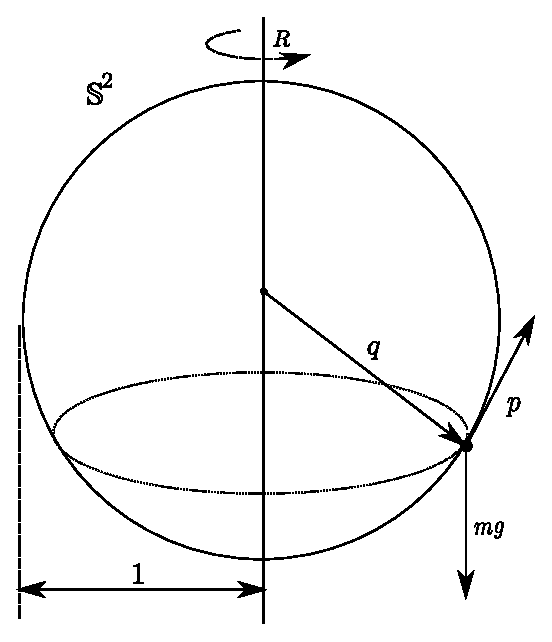
\includegraphics{pics/espendulo.eps}

\vfill

\rm \large
    Facultad de Ciencias Matemáticas \\
    Departamento de Álgebra, Geometría y Topología \\
Dirigido por Jesús M. Ruiz
\end{center}
\end{titlepage}  





\newpage\null\thispagestyle{empty}\newpage

\begin{abstract}

  El objetivo principal de este trabajo es demostrar el teorema de Arnold-Liouville, que da una condición suficiente para saber si un \em sistema mecánico hamiltoniano \em  es \em integrable por cuadraturas\em. Con este propósito, definimos y desarrollamos los conceptos necesarios para el teorema, dando unas nociones elementales sobre \em geometría simpléctica \em  y su aplicación a la Mecánica Clásica.\\
  

\noindent \em Palabras clave: \em Geometría simpléctica, sistemas integrables, teorema de Arnold-Liouville, flujos hamiltonianos, ecuaciones de Hamilton, derivada de Lie, campos dependientes del tiempo.\\

\noindent {\sc Abstract.} The main goal of this work is to prove the Arnold-Liouville theorem, which gives a sufficient condition for a \em hamiltonian mechanical system \em to be \em integrable by quadratures\em. To that end we define and develop the concepts involved in the theorem, giving some elementary notions of \em symplectic geometry \em and its application to Classical Mechanics.\\

\noindent \em Keywords: \em Symplectic geometry, integrable systems, Arnold-Liouville theorem, hamiltonian flows, Hamilton's equations, Lie derivative, time-dependent vector fields.\\
\

\end{abstract}



\newpage\null\thispagestyle{empty}\newpage

\setcounter{tocdepth}{1}
\newpage
\tableofcontents
\newpage\null\thispagestyle{empty}\newpage

\addcontentsline{toc}{chapter}{Introducción}
\section*{Introducción}
Una \em variedad simpléctica \em es una variedad diferenciable de dimensión par en la que se define una forma diferencial $\omega$ cerrada y no degenerada. La \em geometría simpléctica \em es el estudio de las variedades simplécticas y es interesante tanto por sus problemas fundamentales como por su aplicación a la Mecánica Clásica (y por extensión al resto de la Física). La forma $\omega$ induce un isomorfismo entre campos y 1-formas, que nos permite obtener campos tangentes a partir de funciones definidas sobre la variedad. Las variedades simplécticas constituyen entonces una forma natural de visualizar los sistemas mecánicos ya que las \em ecuaciones de Hamilton \em nos permiten ver las leyes del movimiento como campos tangentes de manera intrínseca a la variedad. 

Un \em sistema mecánico integrable por cuadraturas \em  es aquel en el que las ecuaciones del movimiento pueden ser resueltas salvo el cálculo de integrales definidas (cuadraturas), de forma que el problema de estudiar el comportamiento del sistema queda (al menos numéricamente) resuelto. La \em teoría de Arnold-Liouville \em nos ofrece una forma de saber si un sistema mecánico es integrable por cuadraturas mediante el estudio de la variedad simpléctica que lleva asociado.
Tras un desarrollo previo de algunos prerrequisitos de geometría diferencial como son la \em derivada de Lie \em y los \em campos dependientes del tiempo\em, y tras afianzar algunos conceptos del álgebra lineal de los \em espacios vectoriales simplécticos \em (espacios vectoriales en los que se define una forma cuadrática antisimétrica y no degenerada), nos concentramos en el estudio de la geometría simpléctica, para acabar probando los teoremas fundamentales que componen la teoría de Arnold-Liouville.



\section{Motivación física. De Newton a Hamilton} \label{sec:fisica}
La forma más sencilla de describir el movimiento de un sistema de partículas es mediante el formalismo newtoniano, tomando como postulado fundamental de la mecánica clásica el \emph{principio de determinación}: conocidas en cierto instante las posiciones y las velocidades iniciales de todas las partículas que conforman el sistema, es posible determinar sus posiciones y velocidades en cualquier otro instante.

Matemáticamente, este principio se traduce en la existencia de una función\footnote{A lo largo del texto sólo consideraremos funciones diferenciables ($\mathscr{C}^{\infty}$ si es necesario), no lo especificaremos en lo que sigue.}, conocida como \emph{fuerza}, $F: \RR^{3n} \times \RR^{3n} \times \RR \rightarrow \RR$, que cumple la llamada \emph{ecuación de Newton}\footnote{Esta ecuación es una forma peculiar de la conocida \emph{segunda ley de Newton}: $F=ma$.}:
\begin{equation*}
  \ddot{x} = F(x,\dot{x},t;\alpha),
\end{equation*}
donde $n$ es el número de partículas, $x:\RR \rightarrow \RR^{3n}$ es la trayectoria del sistema\footnote{A lo largo del texto utilizaremos la notación usual en Física por la que un punto encima de una función dependiente del tiempo indica la derivada temporal: $\dot{a}=\frac{da}{dt}$. En particular el punto indica que debe existir esa dependencia respecto del tiempo.} y $\alpha$ son unos ciertos parámetros de los que puede depender $F$, como por ejemplo las masas o las cargas eléctricas de las diferentes partículas. Para cada sistema concreto, la fuerza se determina experimentalmente. Desde un punto de vista matemático, decimos que la fuerza define un \emph{sistema mecánico newtoniano}. En general, cuando hablemos de los distintos tipos de sistema mecánico, llamaremos a sus ecuaciones diferenciales asociadas (Newton, Euler-Lagrange, Hamilton) \emph{ecuaciones del movimiento} o \emph{dinámica del sistema}.

El formalismo newtoniano ofrece una forma muy simple de entender los sistemas mecánicos pero tiene la complicación de que es necesario medir y calcular las tres componentes de la posición y de la velocidad de cada partícula que conforma el sistema. Por verlo con un ejemplo, si queremos describir el movimiento de un barco en un viaje transatlántico deberíamos tomar una referencia cartesiana (tal vez el centro de la Tierra y tres ejes perpendiculares) y describir su posición y velocidad en $\RR^3$ en términos de esta referencia, cuando lo que parece más sencillo es simplemente entender el barco como una partícula moviéndose en la superficie de $\SF^2$ y dar su posición y velocidad en términos de su latitud y longitud.
Otro ejemplo lo podemos ver si consideramos el movimiento de una peonza. En este caso, aunque la peonza esté compuesta de cuatrillones de partículas, es posible describir su posición sólo con tres ángulos (el de giro respecto a su eje y los dos de orientación de su eje), o equivalentemente, con la rotación de sus ejes propios respecto a los de una referencia inmóvil exterior (un \emph{sistema de laboratorio}), es decir, con un elemento de $\mathrm{SO}(3)$. 

De forma más general, podemos considerar sistemas newtonianos sometidos a \emph{ligaduras} entre las partículas que lo conforman. Las posibilidades de movimiento quedan entonces restringidas a un subconjunto de $\RR^{3n}$. En el caso de que estas ligaduras sean «lo suficientemente buenas» (\emph{holónomas} es el término clásicamente usado en mecánica), es posible entenderlas como unas funciones $f_1,\dots,f_r: \RR^{3n} \rightarrow \RR$, independientes en todo $x \in \RR^{3n}$ ($d_xf_1 \wedge \cdots \wedge d_xf_r \neq 0$), tales que
\begin{equation*}
  \left\lbrace
  \begin{array}{rl}
    f_1(x)&=0 \\
    &\vdots \\
    f_r(x)&=0.
  \end{array}
  \right.
\end{equation*}
Por el teorema de la función implícita, las ligaduras definen una subvariedad regular $M \subset \RR^{3n}$ de dimensión $m=3n-r$. En Física, a esta $M$ se le suele llamar \emph{espacio de configuración} del sistema y a $m$ su número de \emph{grados de libertad}. Así, llegamos al formalismo lagrangiano. 

Un \emph{sistema lagrangiano} viene dado por una variedad diferenciable $M$ de dimensión $m$. Si $(U,q)$ es una carta en $M$, las coordenadas $q=(q_1,\dots,q_m): U \rightarrow \RR^m$ suelen llamarse en Física \emph{coordenadas generalizadas} del sistema. Dados $x \in M$ y $v \in T_x M$, las coordenadas de $v$ suelen denotarse $\dot{q}=(\dot{q}_1,\dots,\dot{q}_m)$ y suelen llamarse \emph{velocidades generalizadas} del sistema. Esto significa en realidad que, en la carta $(U,q)$, $v=\sum_{i=1}^{m}\dot{q_i}\deriv{q_i}$. Como no hay $t$ respecto de la que derivar, es sólo una notación, pero es consistente. Si $v=\dot{x}(t)$ tenemos
\begin{equation*}
  \dot{q_i} = dq_{i,x(t)}(v)=\frac{d}{dt}(q_i \circ x) (t).
\end{equation*}

Un \emph{estado} del sistema lagrangiano vendrá dado por un punto $(x,v) \in TM$, donde $x$ es la posición y $v$ la velocidad del sistema en dicho estado, y una \emph{trayectoria} del sistema vendrá dada por una aplicación
\begin{equation*}
  \begin{array}{rcl}
    \gamma: \RR & \longrightarrow & TM \\
    t & \longmapsto & (x(t), \dot{x}(t)).
  \end{array}
\end{equation*}
Vemos que esta trayectoria está asociada a una curva $x:\RR \rightarrow M$ en el espacio de configuración, que podemos entender como la descripción de las posiciones de las partículas a lo largo del tiempo, mientras que $\dot{x}(t)=\frac{d}{dt}x(t)$ describe sus velocidades.

La dinámica del sistema lagrangiano viene dada por lo que se conoce como el \emph{principio de mínima acción}. Este principio puede deducirse a partir del formalismo newtoniano, imponiendo ciertas condiciones a las fuerzas y a partir del \emph{principio de D'Alembert} (o \emph{de los trabajos virtuales}), como puede leerse en \cite{goldstein}. Sin embargo, aquí le daremos un enfoque distinto, postulando directamente el principio de mínima acción, al estilo de Landau y Lifshitz \cite{landau}:
  \begin{quote}
    «La formulación más general de la ley del movimiento de los sistemas mecánicos es el \emph{principio de mínima acción} (o \emph{principio de Hamilton}).»
  \end{quote}

  En primer lugar, el principio de mínima acción afirma que todo sistema mecánico viene caracterizado por una función $L: TM \rightarrow \RR$, llamada \emph{lagrangiano} del sistema. Ahora, suponiendo que en los tiempos $t_1$ y $t_2$ el sistema ocupa los estados $(x_1,v_1)$ y $(x_2,v_2)$, la trayectoria que describirá el sistema entre los dos estados será aquella que minimice (o más precisamente, que haga extremal) la integral
  \begin{equation}\label{accion}
    S(\gamma) = \int_{t_1}^{t_2} L(\gamma(t)).
  \end{equation}
  Este funcional $S$ se conoce como la \emph{acción} del sistema.

  Utilizando técnicas de cálculo variacional \cite{arnold}, es posible obtener unas ecuaciones diferenciales para las trayectorias que hacen extremales funcionales de la forma de $S$. Las soluciones de estas ecuaciones son las trayectorias «reales» del sistema lagrangiano. Tenemos así las \emph{ecuaciones de Euler-Lagrange}, que en coordenadas locales se expresan:
  \begin{equation*}
    \left[\frac{d}{dt}\left( \parcial{L}{\dot{q_i}} \right)- \parcial{L}{q_i}\right](t) = 0,    
  \end{equation*}
  para $i=1,\dots,m$.

  \begin{center}  $\ast\ast\ast$ \end{center}
  Dado un sistema newtoniano $F:\RR^{3n}\times\RR^{3n}\times\RR \rightarrow \RR^{3n}$, se define la \emph{energía cinética} como una aplicación
  \begin{align*}
    T: \RR^{3n} & \longrightarrow \RR \\
    v & \longmapsto \thalf \esc{v}{v}.
  \end{align*}
  Decimos que el sistema es \emph{conservativo} o, equivalentemente que $F$ es una \emph{fuerza conservativa} si ésta sólo depende de la posición y además es un campo gradiente, es decir, si existe una función $V:\RR^{3n}\rightarrow \RR$ que cumpla $F(x)=-\nabla V(x)$. Esta $V$ toma el nombre de \emph{energía potencial}.
  En un sistema newtoniano conservativo podemos ver la ecuación de Newton en la forma
  \begin{equation*}
    \frac{d}{dt} \left( \left. \parcial{T}{v_i} \right|_{\dot{x}(t)} \right) = \left.-\parcial{V}{x_i}\right|_{x(t)}, \ \ i=1,\dots,3n.
  \end{equation*}
  Ahora, escribiendo la función $L(x,v)=T(v)-V(x)$, tenemos
  \begin{equation*}
    \left[\frac{d}{dt}\left( \parcial{L}{v_i} \right) - \parcial{L}{x_i}\right]_{(x(t),\dot{x}(t))} = 0, \ \  i=1,\dots,3n.
  \end{equation*}
  Así, podemos ver cualquier sistema newtoniano conservativo como un sistema lagrangiano con $M=\RR^{3n}$ y $L=T-V$.

  En el caso de una variedad diferenciable cualquiera, debemos tener en cuenta que el producto escalar $\esc{u}{v}$ deberá ser sustituido por una métrica riemmaniana $g$. Recordamos que una \emph{métrica riemanniana} en una variedad diferenciable $M$ se define como una colección de productos escalares
  \begin{equation*}
    g_x: T_xM \times T_xM \rightarrow \RR, \ \ x\in M,  
  \end{equation*}
  que satisface la siguiente condición de \emph{diferenciabilidad}: para cada par $X,Y$ de campos tangentes diferenciables de $M$ la función
  \begin{align*}
    \esc{X}{Y}: M & \longrightarrow \RR \\
    x & \longmapsto g_x(X_x,Y_x)
  \end{align*}
  es diferenciable. Se llama \emph{variedad riemanniana} a un par $(M,g)$, donde $M$ es una variedad diferenciable y $g$ una métrica riemanniana en $M$.
  
  Definimos entonces un sistema lagrangiano \emph{natural}, como un par $\left( (M,g), L \right)$, donde $(M,g)$ es una variedad riemmaniana y $L:TM \rightarrow \RR$ es de la forma $L=T-V$, con $T:TM \rightarrow \RR$, $T(x,v)=\thalf g_x(v,v)$ y $V: M \rightarrow \RR$ una función\footnote{Aunque $V(x)$ está definida en $M$, la expresión $L=T-V$ tiene sentido si entendemos $V$ como una función definida en $TM$ con $V(x,v)=V(x)$.}.

  \begin{center}  $\ast\ast\ast$ \end{center}

  Es una técnica común a la hora de estudiar ecuaciones diferenciales de orden 2 \[f''(x)=F(x,f,f'),\] realizar un cambio de la forma
  \begin{equation*}
    \left\lbrace
    \begin{array}{l}
      f'(x)=g(x) \\
      g'(x)=F(x,f,g),
    \end{array}
    \right.
  \end{equation*}
  lo que convierte la ecuación original de orden 2 en un sistema de dos ecuaciones de orden 1. Esto ofrece una serie de ventajas prácticas y fundamentales, ya que nos permite ver la ecuación diferencial como un campo y su solución como el flujo correspondiente. La misma idea se puede aplicar para estudiar sistemas lagrangianos.

  Sea $\left( (M,g), L \right)$ un sistema natural. En $TM$ tenemos las coordenadas $(q,\dot{q})$, pero podemos definir otras usando la dualidad asociada a la métrica riemanniana $g$, es decir, el isomorfismo de Riesz:
  \begin{align*}
    T_xM & \longrightarrow T_xM^* \\
    v & \longmapsto g_x(v,\bullet).
  \end{align*}
  En efecto, las formas 
  \begin{equation*}
    p_i = g_x\left(\deriv{q_i},\bullet\right), \ \ i=1,\dots,m,
  \end{equation*}
  que se llaman \emph{momentos canónicos conjugados} o simplemente \emph{momentos}, son independientes y forman una base de $T_xM^*$, de modo que $p=(p_1,\dots,p_m)$ son coordenadas en $T_xM$. Explícitamente
  \begin{equation*}
    p_i= \sum_{i=1}^{m}p_i\left( \deriv{q_j} \right)\dd q_j = \sum_{i=1}^m g_{ij}\dd q_j,
  \end{equation*}
  es decir, $p_i(q,\dot{q})=\sum_{i=1}^m g_{ij}(q) \dot{q_j}$, donde $g_{ij}(q)$ son las componentes de la matriz asociada a $g_x$ en la base $\left\lbrace \deriv{q_i} \right\rbrace$. Por tanto
  \begin{equation*}
    \parcial{}{\dot{q}_i}p(q,\dot{q})=g_{ji}(q).
  \end{equation*}
  Así, $(q,p)$ son unas nuevas coordenadas en $TM$. Ahora, si recordamos que 
  \begin{equation*}
    L(q,\dot{q})=\thalf\sum_{i,j=1}^m \dot{q}_i g_{ij}(q) \dot{q}_j - V(q),
  \end{equation*}
  resulta que
  \begin{equation*}
    \parcial{L}{\dot{q}_i}=\sum_{j=1}^m g_{ij}(q)\dot{q}_j=p_i(q,\dot{q}).
  \end{equation*}

  Consideramos ahora una función $H:TM\rightarrow \RR$, que en las coordenadas $(q,\dot{q})$ es 
  \begin{equation*}
    H(q,\dot{q})=\sum_{i=1}^m p_i \dot{q_i} - L(q,\dot{q}),
  \end{equation*}
  con las $p$ dadas en función de las $\dot{q}$ mediante la relación $p_i(q,\dot{q})=\sum_{i=1}^m g_{ij}(q) \dot{q_j}$. Derivando a ambos lados de la expresión respecto de $\dot{q}_j$ obtenemos
  \begin{equation*}
    \sum_{i=1}^m \parcial{H}{p_i}\parcial{p_i}{\dot{q}_j}=\sum_{i=1}^m \parcial{p_i}{\dot{q}_j}\dot{q}_i + p_j - \parcial{L}{\dot{q}_j}
  \end{equation*}
  que nos lleva a
  \begin{equation*}
    \sum_{i=1}^m \left( \parcial{H}{p_i}-\dot{q}_i \right)g_{ij}=0.
  \end{equation*}
  Como la matriz $(g_{ij})_{i,j}$ es regular,
  \begin{equation*}
    \parcial{H}{p_i}=\dot{q}_i.
  \end{equation*}
  Si derivamos respecto de $q_j$ tenemos
  \begin{equation*}
    \parcial{H}{q_j}+\sum_{i=1}^m \parcial{H}{p_i}\parcial{p_i}{q_j}= \sum_{i=1}^m \parcial{p_i}{q_j} \dot{q_i} - \parcial{L}{\dot{q}_j}.
  \end{equation*}
  Finalmente, usando la relación recién obtenida,
  \begin{equation*}
    \parcial{H}{q_j}=-\parcial{L}{q_j}.
  \end{equation*}

  Para ver cómo será la dinámica del sistema en estas coordenadas, consideramos una trayectoria $(x(t),\dot{x}(t))$, que en las nuevas coordenadas se expresa $(q(t),p(t))$, con $p(t)=(p_1(t),\dots,p_m(t))$ y $p_i(t)=\sum_{j=1}^m g_{ij}(q(t)) \dot{q_j}(t)$. Nótese que aquí el punto sí expresa derivación respecto del tiempo, es decir, que las $p$ dependen de las $q$. En este caso, por la ecuación de Euler-Lagrange, la segunda de las relaciones anteriores queda:
  \begin{equation*}
    \parcial{H}{q_j}(t)=-\parcial{L}{q_j}(t)=-\left(\frac{d}{dt} \parcial{L}{\dot{q}_j} \right)(t)= - \frac{d}{dt}p_j(t) = -\dot{p}_j(t).
  \end{equation*}
  
  Obtenemos entonces un sistema de EDOs de orden 1 equivalentes a la ecuación de Euler-Lagrange
  \begin{align}
    \begin{cases}
    \dot{q_i}(t)&=\parcial{H}{p_i}(t) \\
      \dot{p_i}(t)&=-\parcial{H}{q_i}(t),
    \end{cases}
    \label{hamilton}
  \end{align}
  para $i=1,\dots,n$. Éstas son las \emph{ecuaciones de Hamilton}.
  
  Si queremos dotar de sentido físico a esta función $H$, conocida como \emph{hamiltoniano} del sistema, consideremos un sistema natural con lagrangiano $L=T-V$. Entonces $p_i=\sum_{j=1}^m g_{ij}(q)\dot{q}_j$ y $T(q,\dot{q})=\sum_{i,j=1}^m\thalf\dot{q}_ig_{ij}(q)\dot{q}_j$, por tanto
\begin{equation*}
  H(q,\dot{q})=\sum_{i=1}^m p_i(q,\dot{q})\dot{q}_i - L(q,\dot{q})=\sum_{i,j=1}^m (g_{ij} \dot{q_j})\dot{q}_i - \thalf\sum_{i,j=1}^m \dot{q}_i g_{ij} \dot{q}_j + V(q)=T(q,\dot{q})+V(q),
\end{equation*}
Es decir, el hamiltoniano es exactamente $T+V$, la \emph{energía total} del sistema.
  
 De esta forma, podemos entender la dinámica de un sistema lagrangiano como la definición de un campo tangente al fibrado tangente del espacio de configuración, cuyas curvas integrales contendrán toda la información sobre la evolución temporal del sistema. En coordenadas locales este campo tangente se expresa
 \begin{equation*}
   X=\sum_{i=1}^m \left( \parcial{H}{p_i}\deriv{q_i}-\parcial{H}{q_i}\deriv{p_i} \right).
 \end{equation*}
  
  \begin{center}  $\ast\ast\ast$ \end{center}
 La siguiente pregunta que cabe hacerse es si será posible construir este campo de forma independiente de las coordenadas a partir de la especificación de un hamiltoniano $H:TM \rightarrow \RR$. La construcción es sencilla, basta considerar un punto $\zeta \in TM$, con coordenadas $(q,p)$ y la 1-forma $\alpha$ que localmente se expresa
 \begin{equation*}
   \alpha = \sum_{i=1}^m p_i \dd q_i.
 \end{equation*}
 Entonces, la 2-forma
 \begin{equation*}
   \omega=\dd \alpha = \sum_{i=1}^m \dd p_i \wedge \dd q_i,
 \end{equation*}
 es cerrada (porque es exacta) y no degenerada. 

Usando esta forma se puede construir un isomorfismo lineal, dado $\zeta \in TM$,
\begin{equation}
  \label{isomorfismo}
  \begin{array}{rcl}
     T_{\zeta}(TM) & \longrightarrow & (T_{\zeta}(TM))^* \\
    \xi & \longmapsto & \omega(\xi, \bullet).
  \end{array}
\end{equation}
Ahora, si $X^H$ es el campo asociado a $\dd H$ por este isomorfismo, es decir, tal que $\dd H=\omega(X^H,\bullet)$, es fácil comprobar que en coordenadas locales se expresará tal y como queríamos:
\begin{equation*}
  X^H = \sum_{i=1}^m \left( \parcial{H}{p_i} \deriv{q_i} - \parcial{H}{q_i} \deriv{p_i} \right).
\end{equation*}
En efecto, si $X^H=\sum_{i=1}^m \left( a_i \deriv{q_i} + b_i \deriv{p_i} \right)$,
\begin{align*}
  a_i&=\omega\left(X^H,\deriv{p_i}\right)=\dd H\left( \deriv{p_i} \right)=\parcial{H}{p_i} \\
  -b_i&=\omega\left(X^H,\deriv{q_i}\right)=\dd H\left( \deriv{q_i} \right)=\parcial{H}{q_i},
\end{align*}
ya que $\dd H = \sum_{i=1}^m\parcial{H}{q_i}\dd q_i + \parcial{H}{p_i}\dd p_i$.

Obsérvese que el único elemento realmente crucial en la construcción de este campo ha sido la 2-forma $\omega$. Una forma de esas características induce sobre $TM$ la estructura de \emph{variedad simpléctica}. El estudio de las variedades simplécticas y sus propiedades es la \emph{geometría simpléctica}. A partir de la sección \ref{sec:vectoriales}, introduciremos el formalismo de la geometría simpléctica, lo que nos permitirá enunciar la \emph{formulación canónica} de la mecánica clásica y resolver alguno de sus problemas.



\section{Derivada de Lie}\label{sec:lie}

Antes de comenzar con el estudio de la geometría simpléctica, conviene recordar el concepto de la derivada de Lie de campos, extenderlo a formas, y obtener una serie de resultados que nos serán útiles más adelante.

Empecemos recordando la definición del corchete de Lie de campos, su estudio detallado puede encontrarse en \cite{variedades}.

\begin{defn}[Corchete de Lie]
  \em
  Sea $M$ una variedad diferenciable y $\mathfrak{X}(M)$ el conjunto de los campos diferenciables en $M$, se define el \emph{corchete de Lie} como la aplicación
  \begin{equation*}
    \begin{array}{rcl}
    \lie{\ }{\ }: \mathfrak{X}(M) \times \mathfrak{X}(M) & \longrightarrow & \mathfrak{X}(M) \\
    (X,Y) & \longmapsto & \lie{X}{Y} = X \circ Y - Y \circ X,
  \end{array}
  \end{equation*}
  donde la composición se entiende si vemos los campos como aplicaciones $\mathcal{C}^{\infty}(M) \rightarrow \mathcal{C}^{\infty}(M)$.
\end{defn}
Recordamos también que podemos ver el corchete de Lie de otra forma equivalente. Sea $M$ una variedad diferenciable, $a \in M$, $Y \in \mathfrak{X}(M)$, $\varphi$ un flujo en $M$ y $X$ su generador infinitesimal. Entonces
\begin{equation*}
  \lie{X}{Y}_a= \lim_{t\rightarrow 0}\frac{\varphi_{-t,*}(Y_{\varphi_t(a)})-Y_a}{t}.
\end{equation*}
En vista de esta fórmula, se define la \emph{derivada de Lie de Y respecto de X} como $L_XY=\lie{X}{Y}$. 
\begin{figure}[h]
  \centering
  \includegraphics{pics/lie}
  \caption{Visión geométrica de la derivada de Lie}
  \label{fig:lie}
\end{figure}
Por último, recordamos otro resultado muy importante que usaremos posteriormente:
\begin{prop}
  Sea $M$ una variedad diferenciable, sean $\varphi$, $\psi$ flujos en $M$ y sean $X$, $Y$ sus generadores infinitesimales, respectivamente. Entonces los flujos conmutan si y sólo si lo hacen sus generadores infinitesimales (es decir, $\varphi_t \circ \psi_s = \psi_s \circ \varphi_t$ si y sólo si $\lie{X}{Y}=0$).
\end{prop} 

Ya estamos en disposición de dar una definición más general de la derivada de Lie:
\begin{defn}[Derivada de Lie]
  \em
  Sean $M$ una variedad diferenciable, $X$ un campo en $M$, y $\varphi$ su flujo. Se define la \emph{derivada de Lie respecto de X} como la aplicación  \begin{equation*}
    \begin{array}{rcl}
    L_X: \Gamma^r(M)& \longrightarrow & \Gamma^r (M) \\
    \omega & \longmapsto & L_X \omega = \lim_{t\rightarrow 0}\frac{\varphi^*_t \omega - \omega}{t}
  \end{array}
  \end{equation*}
  (es decir, $(L_X\omega)_x=\lim_{t\rightarrow 0}\frac{\varphi^*_t\omega_{\varphi_t(x)}-\omega_x}{t}$ para $x \in M$).
\end{defn}

Vamos a obtener ahora un par de propiedades de la derivada de Lie.

\begin{prop}
  Sean $M$ una variedad diferenciable, $\omega \in \Gamma^r(M)$, $X,X_1,\dots,X_r\in \mathfrak{X} (M)$, se cumple
  \begin{equation*}
    L_{X}\omega(X_1,\dots,X_r)=X\omega(X_1,\dots,X_r)-\sum_{i=1}^r \omega(X_1,\dots,\lie{X}{X_i},\dots,X_r)
  \end{equation*}
\end{prop}
\begin{proof}
  Vamos a probarlo sólo para el caso en el que $\omega$ es una 2-forma para simplificar su lectura. El cálculo general es completamente análogo.
  En primer lugar,
  \begin{align*}
    \lim_{t\rightarrow 0}\frac{1}{t}[(\varphi_t^* \omega)(X_1,X_2) - \omega (X_1,X_2)] =\lim_{t\rightarrow 0}\left[\frac{1}{t}[(\varphi_t^* \omega)(X_1,X_2) - \varphi_t^*(\omega(X_1,X_2))]\right] \\
    + \lim_{t\rightarrow 0}\left[\frac{1}{t}[\varphi_t^*(\omega(X_1,X_2))-\omega(X_1,X_2)]\right].
  \end{align*}

  El segundo término de esta expresión es exactamente
  \begin{equation*}
    \lim_{t\rightarrow 0}\left[\frac{1}{t}[\varphi_t^*(\omega(X_1,X_2))-\omega(X_1,X_2)]\right]=\left( \left. \frac{d}{dt}\right|_{t=0} \varphi_t \right)(\omega(X_1,X_2))=X\omega(X_1,X_2),
  \end{equation*}
  mientras que el primer término, en $x\in M$ es
  \begin{align*}
     & \left.\lim_{t\rightarrow 0}\left[\frac{1}{t}[(\varphi_t^* \omega)(X_1,X_2) - \varphi_t^*(\omega(X_1,X_2))]\right]\right|_{x}  \\
     & = \lim_{t \rightarrow 0}\frac{1}{t}[\omega_{\varphi_t(x)}(d_x \varphi_t(X_{1,x}),d_x \varphi_t(X_{2,x})) -\omega_{\varphi_t(x)}(X_{1,\varphi_t(x)},X_{2,\varphi_t(x)})] \\
     & = \lim_{t\rightarrow 0} \omega_{\varphi_t(x)}\left[\frac{1}{t}(d_x \varphi_t(X_{1,x})-X_{1,\varphi_t(x)}),d_x\varphi_t(X_{2,x})\right] + \lim_{t\rightarrow 0} \omega_{\varphi_t(x)}\left[ X_{1,\varphi_t (x)}, \frac{1}{t}(d_x \varphi_t (X_{2,x})-X_{2,\varphi_t(x)}) \right] \\
     & = -\omega_x(\lie{X}{X_1}_x,X_{2,x})-\omega_x(X_{1,x},\lie{X}{X_2}_x).
  \end{align*}
  Comprobemos que, en efecto
  \begin{equation*}
    \lim_{t\rightarrow 0}\tfrac{1}{t}(d_x\varphi_t(X_{1,x})-X_{1,\varphi_t(x)})=\lie{X}{X_1}_x,
  \end{equation*}
  y es análogo para $\lie{X}{X_2}_x$.
  Basta «sacar factor común» a $d_x\varphi_t$, de modo que
  \begin{equation*}
    \tfrac{1}{t}(d_x\varphi_t(X_{1,x})-X_{1,\varphi_t(x)})=-d_x\varphi_t\left( \frac{\left( d_x\varphi_t \right)^{-1}\left( X_{1,\varphi_t(x)} \right)-X_{1,x}}{t} \right).
  \end{equation*}
  Ahora, $(d_x\varphi_t)^{-1}=d_{\varphi_t(x)}\varphi_{-t}=\varphi_{-t,*}$ y 
  \begin{equation*}
    \lim_{t\rightarrow 0} \tfrac{1}{t}(\varphi_{-t,*}(X_{1,\varphi_t(x)})-X_{1,x})=\lie{X}{X_1}_x.
  \end{equation*}

  Volviendo a agrupar, tenemos lo que se quería demostrar.
\end{proof}
\begin{prop}
  Sea $M$ una variedad diferenciable y $\alpha \in \Gamma^r(M)$. Se cumple
  \begin{align*}
    (\dd \alpha)(X_1,\dots,X_{r+1})=\sum_{i=1}^{r+1}(-1)^{i-1}X_i \alpha (X_1,\dots,\hat{X_i},\dots,X_{r+1}) \\
    + \sum_{i<j}(-1)^{i+j}\alpha(\lie{X_i}{X_j},X_1,\dots,\hat{X_i},\dots,\hat{X_j},\dots,X_{r+1}),
  \end{align*}
  donde el circunflejo en un campo quiere decir que este campo se omite.
\end{prop}
\begin{proof}
En este caso probaremos solo la identidad más sencilla 
\begin{equation*}
  \dd \alpha (X,Y) = X\alpha(Y) - Y \alpha(X) - \alpha(\lie{X}{Y}),
\end{equation*}
válida para el caso en el que $\alpha$ es de grado 1. El caso general es completamente análogo.

En primer lugar, escribimos todo en coordenadas locales:
\begin{align*}
  \alpha &= \sum_i \alpha_i \dd \xx _i, \ \dd \alpha = \sum_{i,j} \dd \alpha_i \wedge \dd \xx _j = \sum_{i,j}\parcial{\alpha_i}{\xx_j} \dd \xx_i \wedge \xx_j, \\
  X &= \sum_i X_i \deriv{\xx_i}, \ 
  \lie{X}{Y} = \sum_{i,j} \left( X_i \parcial{Y_j}{\xx_i} - Y_i \parcial{X_j}{\xx_i} \right) \deriv{\xx_j}.
\end{align*}

Ahora, operando en estas coordenadas:
\begin{align*}
  \alpha(X) &= \sum_i \alpha_i X_i, \ 
  \dd \alpha (X,Y) = \sum_{i,j} \parcial{\alpha_i}{\xx_j} (X_jY_i-X_iY_j), \\
  \alpha(\lie{X}{Y}) &= \sum_{i,j} \left( X_i \parcial{Y_j}{\xx_i} - Y_i \parcial{X_j}{\xx_i} \right) \alpha_j = \sum_{i,j} \alpha_i X_j \parcial{Y_i}{\xx_j} - \sum_{i,j}\alpha_i Y_j \parcial{X_i}{\xx_j}, \\
  X(\alpha Y) &= \sum_{i,j}\alpha_i X_j \parcial{Y_i}{\xx_j} + Y_i X_j \parcial{\alpha_i}{\xx_j}, \ 
Y(\alpha X) = \sum_{i,j}\alpha_i Y_j \parcial{X_i}{\xx_j} + X_i Y_j \parcial{\alpha_i}{\xx_j}.
\end{align*}

Obtenemos entonces
\begin{equation*}
  X(\alpha(Y))-Y\alpha(X)-\alpha(\lie{X}{Y}) = \sum_{i,j} Y_iX_j \parcial{\alpha_i}{\xx_j} - X_iY_j \parcial{\alpha_i}{\xx_j} = \dd \alpha (X,Y).
\end{equation*}
\end{proof}

Antes de seguir, vamos a introducir una nueva operación para formas:
\begin{defn}[Producto interior]
  \em
  Sea $M$ una variedad diferenciable y $X$ un campo en $M$, se define el \emph{producto interior} $i_X:\Gamma^{r+1}(M)\rightarrow \Gamma^r(M)$ por 
  \begin{equation*}
    i_X \omega(X_1,\dots,X_r)=\omega(X,X_1,\dots,X_r),
  \end{equation*}
  para $X_1,\dots,X_r \in \mathfrak{X}(M)$.
\end{defn}

Podemos probar ya una serie de fórmulas, debidas a Élie Cartan\footnote{En la literatura, la segunda de estas fórmulas suele llamarse «fórmula mágica de Cartan».}, que nos serán de gran utilidad posteriormente.
\begin{thm}[Fórmulas de Cartan]
  Sea $X$ un campo en una variedad $M$, y consideramos la derivada de Lie $L_X$, el producto interior $i_X$, y la diferencial exterior $\dd$. Entonces se cumplen las siguientes fórmulas:
  \begin{enumerate}
    \item $i_{\lie{X}{Y}}=L_X i_Y - i_Y L_X$, para todo $Y \in \mathfrak{X}(M)$,
    \item $L_X= \dd \circ i_X + i_X \circ \dd $ y
    \item $L_X\circ \dd = \dd \circ L_X$.
  \end{enumerate}
\end{thm}
\begin{proof}\leavevmode
  \begin{enumerate}
    \item Sean $X_1,\dots,X_r \in \mathfrak{X}(M)$, entonces
      \begin{align*}
	L_X[(i_Y \omega) (X_1,\dots,X_r)] =& X \omega(Y,X_1,\dots,X_r)-\sum_{i=1}^r \omega(Y,X_1,\dots,\lie{X}{X_i},\dots,X_r), \\
	i_Y[(L_X \omega) (X_1,\dots,X_r)] =&  X \omega(Y,X_1,\dots,X_r) -\sum_{i=1}^r \omega(Y,X_1,\dots,\lie{X}{X_i},\dots,X_r) \\
	&- \omega(\lie{X}{Y},X_1,\dots,X_r).
      \end{align*}
      Por tanto
      \begin{align*}
	i_{\lie{X}{Y}}\omega (X_1,\dots,X_r) &=\omega(\lie{X}{Y},X_1,\dots,X_r) \\
	&= L_X[(i_Y \omega) (X_1,\dots,X_r)]-i_Y[(L_X \omega) (X_1,\dots,X_r)].
      \end{align*}
    \item Usando la relación entre el corchete de Lie y la diferencial exterior que obtuvimos antes, tenemos
      \begin{align*}
	(\dd (i_X \alpha)) (X_1,\dots,X_r) =& \sum_{i}(-1)^{i-1}X_i \alpha(X,X_1,\dots,\hat{X_i},\dots,X_r) \\
	& + \sum_{i<j} (-1)^{i+j} \alpha (X,\lie{X_i}{X_j},X_1,\dots,\hat{X_i},\dots,\hat{X_j},\dots,X_r),
      \end{align*}
      y
      \begin{align*}
	(i_X (\dd \alpha)) (X_1,\dots,X_r) =& \sum_{i}(-1)^{i}X_i \alpha(X,X_1,\dots,\hat{X_i},\dots,X_r) \\
	& + \sum_{i<j} (-1)^{i+j+1} \alpha (X,\lie{X_i}{X_j},X_1,\dots,\hat{X_i},\dots,\hat{X_j},\dots,X_r) \\
	& + X\alpha(X_1,\dots,X_r) + \sum_j (-1)^{j} \alpha (\lie{X}{X_j},X_1,\dots,\hat{X_j},\dots,X_r).
      \end{align*}
      Sumando ambas expresiones obtenemos
      \begin{align*}
	(\dd i_X \alpha +i_X \dd \alpha) (X_1,\dots,X_r) = & X\alpha(X_1,\dots,X_r) \\
	& + \sum_j (-1)^{j} (-1)^{j-1} \alpha (X_1,\dots,\lie{X}{X_j},\dots,X_r) \\
	= & X\alpha(X_1,\dots,X_r) - \sum_j \alpha (X_1,\dots,\lie{X}{X_j},\dots,X_r). 
      \end{align*}
    \item Utilizando (2) y que $\dd \circ \dd=0$, obtenemos
      \begin{align*}
	L_X \circ \dd &= (i_X \circ \dd) \circ \dd + (\dd \circ i_X) \circ \dd = \dd \circ i_X \circ \dd, \\
	\dd \circ L_X &= \dd \circ (i_X \circ \dd) + \dd \circ (\dd \circ i_X) = \dd \circ i_X \circ \dd,
      \end{align*}
      luego $L_X \circ \dd= \dd \circ L_X$.
  \end{enumerate}
\end{proof}

\section{Campos y formas dependientes del tiempo} \label{sec:tiempo}

  \begin{defn}[Campos y formas dependientes del tiempo] \leavevmode
    \em 
    Sea $ J\subset \RR $ un intervalo abierto y $ M $ una variedad diferenciable:
    \begin{enumerate}
      \item Un \emph{campo tangente (diferenciable) dependiente del tiempo} de $M$ es una aplicación \[\begin{array}{rcl}X:M\times J & \longrightarrow & TM \\ (x,t) & \longmapsto & (x,X_{t,x}) \end{array} \] que es diferenciable como aplicación entre variedades. 
      \item Una \emph{forma diferencial (diferenciable) de grado $r$ dependiente del tiempo} de $M$ es una aplicación \[\begin{array}{rcl} \alpha: M \times J & \longrightarrow & \Lambda^r(M) \\ (x,t) &  \longmapsto & (x,\alpha_{t,x}) \end{array}\] tal que la función \[\begin{array}{rcl} \alpha(X_1,\dots,X_r):M\times J & \longrightarrow & \RR \\ (x,t) & \longmapsto & \alpha_{t,x}(X_{1,x}^t,\dots,X_{r,x}^t)\end{array}\] es diferenciable para cualesquiera $r$ campos $X_1,\dots,X_r \in \mathfrak{X}(M)$.
    \end{enumerate}
  \end{defn}

  \begin{obs}
    \em
    Un campo y una forma dependientes del tiempo se expresan en una carta $(U,\xx)$ en la forma
    \begin{align*}
      X_{t,x} &= \sum X_i(x,t) \left.\deriv{\xx_i}\right|_x \\
      \alpha_{t,x} &= \sum \alpha_i(x,t) \dd \xx_i |_x.
    \end{align*}
    La diferenciabilidad de $X$ y $\alpha$ es equivalente a la de sus componentes $X_i$, $\alpha_i$ como funciones $U\times J \rightarrow \RR$.
  \end{obs}
  Tiene sentido decir ahora qué entendemos por derivar una forma respecto al tiempo. Sea $\alpha_t$ una $r$-forma dependiente del tiempo, la \emph{derivada temporal} de $\alpha_t$ es
    \begin{equation*}
      \left. \frac{d}{dt}\right|_{t=t_0} \alpha_t = \lim_{h\rightarrow 0}\frac{\alpha_{t_0+h}-\alpha_{t_0}}{h}.
    \end{equation*}

%  \begin{defn}
%    \em
%    Sea $U\subset M$ abierto, una \emph{isotopía} de $M$ es una aplicación diferenciable
%	$G: [0,1] \times U\subset M \rightarrow M$
%	tal que $G(0,\bullet)=\varphi_0$ es la identidad y $G(t,\bullet)=\varphi_t$ es un difeomorfismo local. 
%  \end{defn}
%  \begin{defn}
%    \em
%    Sea $G$ una isotopía de una variedad $M$, se define el \emph{generador infinitesimal de G} como el campo tangente dependiente del tiempo que, para $x\in M$ satisface
%    \begin{equation*}
%      X^t_x=\left.\frac{d}{ds}\right|_{s=t}\varphi_s(\varphi_t^{-1}(x)),
%    \end{equation*}
%    es decir
%    \begin{equation*}
%      X^t\circ \varphi_t = \frac{d}{dt} \varphi_t. 
%    \end{equation*}
%  \end{defn}
%
%  \begin{obs}
%    \em
%    Podemos entender las isotopías como «flujos dependientes del tiempo», que se diferencian de los flujos en que pierden la propiedad de semigrupo.
%  \end{obs}
%
%  Podemos ver un campo dependiente del tiempo $X_t$ en $M$ como un campo independiente del tiempo
%  \begin{equation*}
%    \begin{array}{rcl}
%    \tilde{X}: M \times [0,1] & \longrightarrow & T(M \times [0,1]) \\
%    (x,t) &\longmapsto& \left( (x,t),X^t_x+\left.\deriv{\mathtt{t}}\right|_t \right).
%  \end{array}
%  \end{equation*}
%  Si $X_t$ tiene soporte compacto y existe $x_0 \in M$ tal que $X^t_x=0$ para cada $t\in[0,1]$, entonces $\tilde{X}$ tiene soporte compacto y genera un flujo completo $\Phi_s(x,t)$ en $(U \subset M) \times [0,1]$, donde $U$ es un entorno de $x_0$. Podemos definir entonces una isotopía $G:[0,1]\times U \rightarrow M$, donde $G(s,x)=\varphi_s(x)$ es la primera componente de $\Phi_s(x,0)$. Claramente es una isotopía porque la primera componente de $\Phi_0(\bullet,0)$ es la identidad en $M$ y la de $\Phi_s(\bullet,0)$ es un difeomorfismo local. Además, 
%  \begin{equation*}
%    \Phi_s(x,t)=\Phi_{s+t}\circ(\Phi_t)^{-1}(x,t)=\Phi_{s+t}\left( \varphi_t^{-1}(x),0 \right)=(\varphi_{s+t}\circ\varphi_t^{-1}(x),t+s)
%  \end{equation*}
%  Ahora,
%  \begin{equation*}
%    X_x^t+\left.\deriv{\mathtt{t}}\right|_t=\tilde{X}_{(x,t)}=\left.\frac{d}{ds}\right|_{s=0}\Phi_s(x,t)=\left.\frac{d}{ds}\right|_{s=0}\varphi_{t+s}(\varphi_t^{-1}(x))+\left.\deriv{\mathtt{t}}\right|_t,
%  \end{equation*}
%  luego $X^t_x =\left.\frac{d}{ds}\right|_{s=t}\varphi_s(\varphi_t^{-1}(x))$, es decir, $X$ es el generador infinitesimal de la isotopía $G$.

  El siguiente teorema nos permite integrar campos dependientes del tiempo:
  \begin{thm}
    Sea $X:J\times M \rightarrow TM$ un campo dependiente del tiempo. Existen un abierto $V\subset J\times J\times M$ y una función $\varphi:V\rightarrow M$ tal que para cada $s\in J$ y para cada $x\in M$, el conjunto $V^{(s,x)}=\left\{ t\in J | (t,s,x) \in V \right\}$ es un intervalo abierto que contiene a $s$ y la curva $\gamma:V^{(s,x)}\rightarrow M$ definida por $\gamma(t)=\varphi(t,s,x)$ es la única solución maximal al problema de valor inicial
    \begin{align*}
      \gamma'(t)&=X_{t,\gamma(t)}, \\
      \gamma(s)&=x.
    \end{align*}
  \end{thm}
    Equivalentemente, podemos ver el problema de valor inicial en la siguiente forma:
    \begin{align*}
      \parcial{\varphi}{t}(t,s,x)&=X_{t,\varphi(t,s,x)}, \\
      \varphi(s,s,x)&=x.
    \end{align*}
    Esta $\varphi$ recibe el nombre de \emph{flujo dependiente del tiempo}. Nótese que cada $\varphi(t,s,\bullet)$ es una aplicación diferenciable de un abierto de $M$ en $M$, pero no tiene por qué ser un difeomorfismo, es decir, en general el flujo no es completo.

  Ahora podemos generalizar la derivada de Lie de formas para campos dependientes del tiempo:
  \begin{equation*}
    L_{X_{t}}\alpha=\lim_{h\rightarrow 0}\frac{\varphi^*_{t+h,t} \alpha - \alpha}{h},
  \end{equation*}
  para $x\in M$.
  
  Finalmente, tenemos una fórmula que nos relaciona la derivada temporal con la derivada de Lie de formas.
  \begin{prop}
    Sea $ X:J\times M \rightarrow TM $ un campo dependiente del tiempo y $ \varphi:V\rightarrow M $ el flujo dependiente del tiempo asociado. Si $\alpha_t$ es una $r$-forma dependiente del tiempo, entonces para cualquier $(t_1,t_0,x)\in V$ 
   \begin{equation*}
     \left.\frac{d}{dt}\right\lvert _{t=t_1}\left(\varphi^*_{t,t_0} \alpha_t\right)_x = \left(\varphi^*_{t_1,t_0} \left( L_{X_{t_1}}\alpha_{t_1} + \left.\frac{d}{dt}\right\lvert_{t=t_1}\alpha_t\right) \right)_x,
   \end{equation*}
   donde $\varphi_{t,s}=\varphi(t,s,\bullet)$. 
\end{prop}
\begin{obs}
  \em
   Podemos ver esta fórmula en una notación más compacta:

    \begin{equation*}
      \frac{d}{dt}\varphi^*_t \alpha_t = \varphi^*_t \left( L_{X_t}\alpha_t + \frac{d}{dt}\alpha_t \right).
    \end{equation*}
  \end{obs}

  \begin{proof}
    En primer lugar, probaremos la forma más sencilla, en la que $\alpha$ no depende del tiempo,
    \begin{equation*}
      \left.\frac{d}{dt}\right|_{t=t_1}(\varphi^*_{t,t_0}\alpha)=\varphi^*_{t_1,t_0}(L_{X_{t_1}}\alpha).
    \end{equation*}
    En efecto
    \begin{equation*}
      \left.\frac{d}{dt}\right|_{t=t_1}(\varphi_{t,t_0}\alpha)=\lim_{h\rightarrow 0}\frac{\varphi^*_{t_1+h,t_0}\alpha-\varphi^*_{t_1,t_0}\alpha}{h}=\varphi^*_{t_1,t_0}\left( \lim_{h\rightarrow 0 }\frac{\varphi_{t_1+h,t_1}\alpha-\alpha}{h} \right)=\varphi^*_{t_1,t_0}(L_{X_t}\alpha).
    \end{equation*}







  \end{proof}

%
\section{Espacios vectoriales simplécticos}\label{sec:vectoriales}
En esta sección repasamos algunos conceptos de álgebra lineal necesarios para estudiar geometría simpléctica. Introduciremos la noción de \emph{espacio vectorial simpléctico} y veremos algunas de sus propiedades. Muchos de los resultados aquí expuestos pueden leerse más desarrollados en \cite{algebra}.
\begin{defn}[Espacio vectorial simpléctico]
  \em
Un \emph{espacio vectorial simpléctico} es un par ordenado $(V,\omega)$, donde $V$ es un espacio vectorial sobre $\RR$ y 
	\[
	  \omega: V \times V \rightarrow \RR
	\]
	es una forma bilineal antisimétrica no degenerada.
\end{defn}

\paragraph{\bf Clasificación de formas bilineales antisimétricas}
  \begin{enumerate}
    \item Sean $\omega$ una forma bilineal antisimétrica sobre un espacio vectorial $V$ de dimensión finita y $M$ su matriz asociada. Entonces existe $n \leq \frac{1}{2}\dim(V)$ tal que $M$ es congruente con
      \[
	\left(
	\begin{array}{ccc}
	  0 & I_n & 0 \\
	  -I_n & 0 & 0 \\
	  0 & 0 & 0
	\end{array}\right),
      \]
      donde $I_n$ es la matriz identidad $n \times n$.
    \item Si $(V,\omega)$ es un espacio vectorial simpléctico de dimensión finita, entonces $\dim(V)=2n$ para cierto $n \in \NN$.
    \item Sea $(V,\omega)$ un espacio vectorial simpléctico. Se dice que $\mathcal{B}\subset V$ es una \emph{base simpléctica} de $V$ si la matriz asociada a $\omega$ en $\mathcal{B}$ es
\[
  J_n :=
\left(
	\begin{array}{cc}
	  0 & I_n  \\
	  -I_n & 0 
	\end{array}\right).
      \]
    \item Podemos ver la forma bilineal $\omega$ de matriz asociada $J_n$ como una $2$-forma alternada en $V$. Si $\{u_1,\dots,u_n,v_1,\dots,v_n\}$ es una base simpléctica y $\{\varphi_1,\dots, \varphi_n, \psi_1,\dots, \psi_n \}$ es su base dual, entonces
  \[
    \omega = \sum_{i=1}^n \left(\sum_{\sigma \in \mathfrak{S}_2} (-1)^{\sigma} (\psi_i \otimes \varphi_i)^{\sigma}\right)= \sum_{i=1}^n \psi_i \wedge \varphi_i.
  \]
  \item Llamaremos \emph{$n$-ésima forma simpléctica estándar} a la forma $\omega_n:\RR^{2n} \rightarrow \RR^{2n}$ de matriz asociada $J_n$ en la base canónica de $\RR^{2n}$. Llamaremos \emph{espacio simpléctico estándar $n$-dimensional} a $(\RR^{2n},\omega_n)$. Deducimos también de lo anterior que todo espacio vectorial simpléctico de dimensión $2n$ es isomorfo a $(\RR^{2n},\omega_n)$.
\end{enumerate}
\paragraph{\bf Aplicaciones simplécticas}\mbox{}

  Sean $(V,\omega)$ y $(V',\omega')$ espacios vectoriales simplécticos, decimos que una aplicación lineal $f:V \rightarrow V'$ es \emph{simpléctica} si
  \[
    \omega'(f(v),f(w)) = \omega(v,w)
  \]
  para cualesquiera $v,w \in V$.

Ahora, si $w\neq 0$ y $f(v)=0$, entonces $\omega(v,w)=0$ y, como $\omega$ es no degenerada, $v=0$, de modo que $\ker f=\{0\}$. Es decir, toda aplicación simpléctica es inyectiva.

En el caso en que $V$ y $V'$ tienen la misma dimensión, entonces $f$ es un isomorfismo que lleva una base simpléctica de $(V,\omega)$ a una base simpléctica de $(V',\omega')$. 

\paragraph{\bf El grupo simpléctico}\mbox{}

  Sea $(V,\omega)$ un espacio vectorial simpléctico de dimensión $2n$. El conjunto de las aplicaciones lineales simplécticas de $V$ en $V$ es un subgrupo de $\mathrm{GL}(2n)$. Este grupo se conoce como \emph{$n$-ésimo grupo simpléctico} y se denota por $\mathrm{Sp}(n)$.

  Asignando a cada $f\in \mathrm{Sp}(n)$ su matriz asociada $A$ en cierta base, el grupo simpléctico se puede representar por medio de las matrices $2n\times 2n$ que cumplen
  \begin{equation*}
    J_n=A^tJ_n A.
  \end{equation*}
  Estas matrices se dicen \emph{matrices simplécticas}.
  De aquí deducimos inmediatamente, por un razonamiento análogo al que haríamos para matrices ortogonales, que todas las matrices simplécticas tienen determinante $1$ o $-1$. Sin embargo, podemos probar un resultado aún más fuerte sobre el grupo simpléctico: su \emph{subgrupo especial} (es decir, el subgrupo de las aplicaciones de determinante $1$) coincide con él mismo.
\begin{prop}
  Toda aplicación lineal simpléctica tiene determinante $1$.
\end{prop}
\begin{proof}
  Sea $\omega_n$ la forma simpléctica canónica, $\Omega=\omega_n \wedge \overset{(n)}{\cdots} \wedge \omega_n$ es una forma de grado máximo, luego, por el teorema del determinante, $f^*(\Omega)=\det(f) \Omega$. Ahora, como $f$ es simpléctica, 
  \begin{equation*}
    f^*(\Omega) = (\omega_n \circ f) \wedge \overset{(n)}{\cdots} \wedge (\omega_n \circ f)=\omega_n \wedge \overset{(n)}{\cdots} \wedge \omega_n = \Omega.
  \end{equation*}
  Por tanto, $\det(f)=1$.
\end{proof}
\section{Variedades simplécticas y simplectomorfismos}\label{sec:variedades}
\begin{defn}[Variedad simpléctica]
  \em
  Una \emph{variedad simpléctica} es un par ordenado $(M,\omega)$ donde $M$ es una variedad diferenciable de dimensión $2n$ y $\omega \in \Gamma^2(M)$ es cerrada y no degenerada (para todo $x \in M$ y para todo $\xi \in T_xM$ existe $\eta \in T_xM$ tal que $\omega(\xi,\eta)\neq0)$. 
\end{defn}
\begin{defn}[Carta simpléctica]
  \em
  Sea $(M,\omega)$ una variedad simpléctica, una \emph{carta simpléctica en torno a un punto $x \in M$} es un par $(U,(q,p))$, donde $U\subset M$ es un entorno de $x$ y $(q,p)=(q_1,\dots,q_n,p_1,\dots,p_n)$ es un sistema de coordenadas en $x$ tal que:
\begin{equation}
  \omega= \sum_{i=1}^n \dd p_i \wedge \dd q_i.
  \label{forma}
\end{equation}
\end{defn}

Vamos a probar ahora uno de los resultados fundamentales de la geometría simpléctica, que confirma una de las intuiciones que podríamos tener: toda variedad simpléctica es localmente como un espacio vectorial simpléctico.

\begin{thm}[Darboux]
  Sea $\omega$ una $2$-forma no degenerada en una variedad $M$ de dimensión $2n$. Entonces $\omega$ es cerrada si y sólo si para cada $x\in M$ hay una carta $(U,(q,p))$ en torno a $x$, donde $(q,p)=(q_1,\dots,q_n,p_1,\dots,p_n)$ es un sistema de coordenadas que cumple \eqref{forma}. 
\end{thm}
\begin{proof}
  En primer lugar, inmediatamente si $\omega$ tiene esa forma entonces es cerrada. El procedimiento a seguir para demostrar la otra implicación del teorema es el siguiente:
  \begin{enumerate}
    \item Vamos a encontrar un entorno $U \subset M$ y un difeomorfismo $\varphi : U \rightarrow \RR^{2n}$ tal que $\omega_1= (\varphi^*)^{-1}\omega$ es una forma bilineal antisimétrica con coeficientes constantes en $\RR^{2n}$.
    \item Tomamos $\psi: \RR^{2n} \rightarrow \RR^{2n}$ un cambio de base tal que la matriz asociada a $\omega_1$ en la nueva base es $J_n$. 
    \item Tomamos como sistema de coordenadas $(q,p)=\psi \circ \varphi$, entonces $(U,(q,p))$ es una carta simpléctica en torno a $x$.
  \end{enumerate}

\begin{center}
\begin{tikzpicture}
\node (A) at (-2.5,2) {$U$};
\node (B) at (-1,2) {$\RR^{2n}$};
\node (C) at (-1,0) {$\RR^{2n}$};
\node (D) at (1,2) {$ \omega$};
\node (E) at (3,2) {$\omega_1$};
\node (F) at (3,0) {$\omega_n$};
\path[->,font=\scriptsize, >=angle 90]
(A) edge node[above]{$\varphi$} (B)
(A) edge node[left]{$(q,p)$} (C)
(B) edge node[right]{$\psi$} (C);
\path[<-|,font=\scriptsize, >=angle 90]
(D) edge node[left] {$ (q,p) ^*$} (F)
(D) edge node[above] {$\varphi^*$} (E)
(E) edge node[right] {$\psi^*$} (F);
\end{tikzpicture}
\end{center}

  Falta hallar $\omega_1$ y $\varphi$. Sea $\omega_1=\omega_x$, que tiene coeficientes constantes, y sea
  \begin{equation*}
    \omega_t=t\omega_1 + (1-t) \omega = \omega + t(\omega_1-\omega),
  \end{equation*}
  para cada $t\in \RR$. Como $\omega_{t,x}=\omega_x$, para todo $t \in \RR$, $\omega_t$ es no degenerada en $x$. Por tanto, sea $J$ intervalo abierto acotado tal que $[0,1]\in J$, existe un entorno $U \subset M$ de $x$ en el que $\omega_t$ es no degenerada para cada $t\in \bar{J}$.

  Ahora, como $\omega_1-\omega$ es cerrada, podemos tomar $U$ tal que sea difeomorfo a $\RR^{2n}$, luego existirá una 1-forma $\alpha$ en $U$ tal que $\omega_1-\omega=\dd \alpha$. Además, como $\alpha$ está definida salvo una constante, podemos asumir $\alpha_x=0$.

  Para $t \in J$, sea $X_t$ el campo dependiente del tiempo tal que $i_{X^t}\omega_t= - \alpha$ y con $X_{t,x}=0$. Ahora, si $\varphi:V\rightarrow U$ es el flujo dependiente del tiempo asociado a $X$, entonces $\varphi(t,0,x)=x$ para todo $t\in J$, luego $J\times \left\{ 0 \right\}\times \left\{ x \right\} \subset V$. Como $V$ es abierto en $J\times J\times M$ y $[0,1]$ es compacto, existe un entorno $U_0$ de $x$  tal que $[0,1]\times \left\{ 0 \right\}\times U_0 \subset V$. 
  
  Por tanto, si $\varphi_t = \varphi(t,0,\bullet)$ para cada $t\in [0,1]$ se sigue
  \begin{align*}
    \frac{d}{dt}(\varphi_t^*\omega_t) & = \varphi_t^* (L_{X_t}\omega_t) + \varphi_t^* \left( \frac{d}{dt}\omega_t \right) = \varphi_t^* (i_{X_t}(\dd \omega)+\dd (i_{X_t}\omega))+\varphi_t^*(\omega_1-\omega) \\
    & = \varphi_t^*(0-\dd \alpha + \omega_1 - \omega) = 0,
  \end{align*}
  donde hemos usado la fórmula de Cartan. De modo que $\varphi_1^*\omega_1=\varphi_0^*\omega_0=\omega$. Además, como $\varphi_1^*$ es simpléctica, es un isomorfismo, lo que implica que $\varphi_1$ es un difeomorfismo local. Así, reduciendo el entorno si es necesario, encontramos la carta que estábamos buscando.
\end{proof}

Vamos a dar ahora dos propiedades fuertes de las variedades simplécticas:
\begin{prop}
  Toda variedad simpléctica es orientable.
\end{prop}
\begin{proof}
  Como $\omega$ es no degenerada, $\omega^n=\omega \wedge \overset{(n)}{\cdots} \wedge \omega$ es una forma de grado máximo nunca nula, luego la variedad es orientable.
\end{proof}
\begin{prop}
  Si $(M,\omega)$ es una variedad simpléctica compacta y sin borde, entonces su segundo grupo de cohomología de de Rham es no trivial.
\end{prop}
\begin{proof}
  Consideramos en $M$ la forma de volumen $\Omega=\frac{1}{n!}\omega^n$. Ahora, si $\omega=\dd \alpha$, entonces $\omega^n=\dd (\alpha \wedge \omega^{n-1})$. Por el teorema de Stokes
  \begin{equation*}
    \text{Vol}(M)=\int_M \Omega=\int_M \dd (\alpha \wedge \omega^{n-1}) = \int_{\partial M=\varnothing} \alpha \wedge \omega^{n-1}=0,
  \end{equation*}
  que es absurdo porque el volumen de $M$ no puede ser 0. Por tanto, $\omega$ es cerrada y no es exacta, luego $[\omega]\neq 0$ y $H^2(M) \neq \{0\}$.
\end{proof}
\begin{corol}
  $\SF^{2n}$ admite una estructura simpléctica si y sólo si $n=1$.
\end{corol}
\begin{proof}
  Sean $\omega$ una 2-forma en $\SF^n$, $n>2$, $x\in \SF^n$ y $U$ un disco entorno de $x$ ($U \simeq \RR^n$). Entonces existe una 1-forma $\alpha$ definida en $U$ tal que $\omega=\dd \alpha$ en $U$. Sea $\theta$ una función meseta que valga 1 en $U$ y $0$ fuera de un entorno $V$ de $U$, la forma 
  \begin{equation*}
    \omega_1=\omega - \theta \dd \alpha
  \end{equation*}
  es cerrada con soporte compacto en $\SF^n \backslash \{x\}$, que es difeomorfa, por proyección estereográfica $\varphi$, a $\RR^n$. Por tanto, existe una 1-forma $\beta$ de $\RR^n$ tal que $\dd \beta = \varphi^* \omega_1$. Con todo esto, tenemos
  \begin{equation*}
    \omega=\dd\left(\theta \alpha + \left( \varphi^{-1} \right)^* \beta \right) ,
  \end{equation*}
  luego $\omega$ es exacta en $\SF^n$ y 
  \begin{equation*}
    H^2(\SF^n)= \{0\}.
  \end{equation*}
  Si $n=2$, como $\SF^2$ es conexa, compacta y sin borde,
  \begin{equation*}
    H^2(\SF^2)=H^0(\SF^2)=\RR.   
  \end{equation*}
  Por la proposición anterior, si $\SF^{2n}$ admitiera una estructura simpléctica tendría que ser $H^2(\SF^{2n}) \neq \{0\}$, que solamente se da en el caso $n=1$.
\end{proof}

Para terminar la sección, vamos a estudiar los isomorfismos en la categoría de las variedades simplécticas:
\begin{defn}[Simplectomorfismo]
  \em
  Sea $(M,\omega)$ una variedad simpléctica y $f:M \rightarrow M$ un difeomorfismo. Decimos que $f$ es un \emph{simplectomorfismo} o una \emph{transformación canónica} \footnote{Esta nomenclatura es más común en Física} si
  \begin{equation*}
    f^* \omega = \omega
  \end{equation*}
\end{defn}
\begin{prop}
  Sea $(M,\omega)$ una variedad simpléctica y $f:M \rightarrow M$ un difeomorfismo. Son equivalentes:
  \begin{enumerate}
    \item $f$ es un simplectomorfismo.
    \item Para cada $x\in M$, la aplicación lineal $d_xf: \RR^{2n} \rightarrow \RR^{2n}$ es simpléctica.
    \item Para cada $x \in M$, si $(U,(q,p))$ es una carta simpléctica en torno a $x$, $(f(U),(q\circ f, p \circ f))$ es una carta simpléctica en torno a $f(x)$.
  \end{enumerate}
\end{prop}
\begin{proof}\leavevmode
  
  (1) $\implies$ (2):
  \begin{equation*}
    \omega_x=(f^*\omega)_x=\omega_{f(x)} \circ d_x f,
  \end{equation*}
  donde $\omega_x$ es una forma bilineal antisimétrica no degenerada en $T_xM$ y $\omega_{f(x)}$ lo mismo en $T_{f(x)}M$. Tomando bases simplécticas $\mathcal{B}$ y $\mathcal{B'}$ en $T_xM$ y $T_{f(x)}M$, respectivamente, las formas $\omega_x$, $\omega_{f(x)}$ quedan en la forma canónica $\omega_n$. Por tanto
  \begin{equation*}
   \omega_n = \omega_n \circ d_x f, 
  \end{equation*}
  luego $d_x f$ es una aplicación lineal simpléctica.

  (2) $\implies$ (1):

  Si $d_x f$ es simpléctica, para cada $x \in M$ en las bases adecuadas tenemos
  \begin{equation*}
    \omega_x=\omega_{f(x)} \circ d_x f=(f^*\omega)_x. 
  \end{equation*}
Como esto es válido para todo $x \in M$, $\omega=f^* \omega$.

(1) $\Longleftrightarrow$ (3):

\begin{equation*}
  \sum_{i=1}^n \dd (p_i \circ f) \wedge \dd (q_i \circ f) = \sum_{i=1}^n f^* (\dd p_i \wedge \dd q_i) = f^* \left( \sum_{i=1}^n \dd p_i \wedge \dd q_i \right) = f^* \omega
\end{equation*}
es igual a $\omega$ si y sólo si $f$ es un simplectomorfismo.

\end{proof}

Enunciamos también una propiedad inmediata de los simplectomorfismos:
\begin{prop}\label{volumen}
  Los simplectomorfismos preservan el elemento de volumen $\Omega=\frac{1}{n!}\omega^n$.
\end{prop}

\section{Campos y flujos hamiltonianos}\label{sec:hamilton}
\begin{obs}
  \em
  Sea $M$ una variedad simpléctica, la aplicación 
  \begin{equation*}
    \begin{array}{rcl}
      J=I^{-1}: T_xM & \longrightarrow & (T_xM)^* \\
      \xi & \longmapsto & \omega(\xi,\bullet),
      \end{array} 
  \end{equation*}
da un isomorfismo lineal entre campos y 1-formas, a cada campo $X$ le podemos asignar la forma $i_X \omega$.
\end{obs}
\begin{defn}[Campo hamiltoniano y flujo hamiltoniano]
  \em
  Sea una función $H:M \rightarrow \RR$, se llama \emph{campo hamiltoniano generado por H} a 
  \begin{equation*}
    X^H=I \dd H.
  \end{equation*}
  Se llama \emph{flujo hamiltoniano generado por H} y se denota por $\varphi^H$ al flujo cuyo generador infinitesimal es $X^H$.
\end{defn}
\begin{obs}
  \em
  $\dd H = i_{X^H}\omega$
\end{obs}
\begin{obs}
  \em
  Obtenemos ahora una versión geométrica e independiente de las coordenadas de las clásicas ecuaciones de Hamilton:
  \begin{equation*}
    X^H_x= \left.\frac{d}{dt}\right| _{t=0}\varphi^H_t(x).
  \end{equation*}
\end{obs}
Podemos dar ahora una formulación canónica de la mecánica clásica:
\begin{defn}[Sistema hamiltoniano]
  \em
  Un \emph{sistema mecánico hamiltoniano} es un par $(M,H)$, donde $M$ es una variedad simpléctica (comúnmente llamada \emph{espacio de fases}) y $H:M \rightarrow \RR$ es una función (normalmente llamada \emph{hamiltoniano} del sistema).

  Se llama \emph{flujo hamiltoniano del sistema} o \emph{evolución temporal del sistema} al flujo hamiltoniano generado por $H$.
\end{defn}

\begin{ejemplo}
  \em
  Consideremos el espacio simpléctico canónico $(\RR^{2n},\omega_n)$, con un hamiltoniano $H:\RR^{2n}\rightarrow \RR$. Podemos escribir un punto $x\in \RR^{2n}$ en coordenadas simplécticas $x = (q_1,\dots,q_n,p_1,\dots,p_n)$ y el hamiltoniano $H(q_1,\dots,q_n,p_1,\dots,p_n)$. Podemos escribir entonces
  \begin{equation*}
    \dd H = \sum_{i=1}^n \parcial{H}{q_i} \dd{q_i} + \parcial{H}{p_i} \dd{p_i}
  \end{equation*}
  y el campo hamiltoniano tendrá la forma
  \begin{equation*}
    X^H = \sum_{i=1}^n X_{q_i}^H \deriv{q_i} + X_{p_i}^H \deriv{p_i}.
  \end{equation*}
  Ahora, 
  \begin{equation*}
    \dd H = i_{X^H}\omega_n = \sum_{i=1}^n \dd p_i \wedge \dd q_i \left(X_{q_i}^H \deriv{q_i} + X^H_{p_i} \deriv{p_i}\right)  = \sum_{i=1}^n X_{q_i}^H \dd p_i -X_{p_i}^H \dd q_i.
  \end{equation*}
  Por tanto, las componentes del campo hamiltoniano son $X^H_{q_i}=\parcial{H}{p_i}$ y $X^H_{p_i}=-\parcial{H}{q_i}$.

  El flujo hamiltoniano tendrá la forma $\varphi^H_t(x) = (q_1(t),\dots,q_n(t),p_1(t),\dots,p_n(t))$. Luego su generador infinitesimal será de la forma $X^H_x=(\dot{q_1}(t),\dots,\dot{q_n}(t),\dot{p_1}(t),\dots,\dot{p_n}(t))$. Obtenemos entonces las ecuaciones de Hamilton en su forma clásica:
  \begin{align*}
     \dot{q_i}(t) & = \parcial{H}{p_i}(t) \\
     \dot{p_i}(t) & = -\parcial{H}{q_i} (t),
  \end{align*}
  para $i=1,\dots,n$.
\end{ejemplo}

\begin{prop}
  Los flujos hamiltonianos son familias uniparamétricas de simplectomorfismos, es decir, el flujo hamiltoniano preserva $\omega$.
\end{prop}
\begin{proof}
  Sea $X^H$ un campo hamiltoniano, por la fórmula de Cartan,
  \begin{equation*}
    L_{X^H}\omega= \dd (i_{X^H}\omega) + i_{X^H}(\dd \omega) = \dd (\dd H) + 0 = 0.
  \end{equation*}
\end{proof}
Una consecuencia inmediata de este teorema es el conocido resultado de Liouville:
\begin{corol}[Teorema de Liouville]
  El flujo hamiltoniano preserva el volumen del espacio de fases.
\end{corol}
\begin{proof}
  Claramente, como el flujo hamiltoniano consiste en simplectomorfismos y estos preservan el elemento de volumen (proposición \ref{volumen}), entonces el volumen total se preserva con el flujo hamiltoniano.
\end{proof}
A la vista de este resultado, vamos a probar un teorema muy importante sobre transformaciones que preservan el volumen:
\begin{prop}[Teorema de recurrencia de Poincaré \footnote{En inglés \textit{Poincaré recurrence theorem}. Nótese que aquí la palabra «recurrencia» no toma el significado habitual en matemáticas (por ejemplo en «construcción de sucesiones por recurrencia»), que se traduce del inglés \textit{recursion}. El diccionario Oxford define \textit{recursion} como \textit{``the repeated application of a recursive procedure or definition''}. Por otro lado, define \textit{recurrence} como \textit{``the fact of ocurring again''}, que podría traducirse también como «repetición» o «reaparición».}]
 Sea $D\in \RR^n$ acotado y sea $g:D\rightarrow D$ que preserva el volumen. Entonces, para cualquier $U\subset D$ abierto, hay un punto $x\in D$ y un $n\in \NN$, $n>0$, tal que $g^n(x) \in U$.
\end{prop}
\begin{proof}
  Consideramos la familia
  \begin{equation*}
    \{g^nU | n \in \NN \}.
  \end{equation*}
  Todos estos conjuntos tienen el mismo volumen y, si no se cortaran en ningún punto, $D$ tendría volumen infinito. Por tanto, existen $k,l\in \NN$, $k>l$ tal que
  \begin{equation*}
    g^kU\cap g^lU \neq \varnothing.
  \end{equation*}
  Por tanto, $A=g^{k-l}U \cap U \neq \varnothing$. Entonces, sea $y\in A$, existen $x \in U$ y $n=k-l$ tal que $y=g^n(x)\in U$.
\end{proof}
\begin{ejemplo}
  \em
  Sea $D$ una circunferencia y $g$ la rotación de ángulo $\alpha$. Si $\alpha=2\pi(m/n)$, entonces $g^n$ es la identidad y el resultado es obvio. Pero, si $\alpha$ es un múltiplo irracional de $2\pi$, entonces, por el teorema de recurrencia de Poincaré, para todo $x\in D$ y para todo $\delta>0$ existe un $n\in \NN$ tal que $g^n(x) \in B_{\delta}(x)$.
  De aquí se sigue que, dado $x \in D$, el conjunto $\{g^k(x)|k\in \NN\}$ es denso en $D$. Más adelante veremos una aplicación de este ejemplo a mecánica hamiltoniana.

\end{ejemplo}

Para terminar la sección, haremos un breve comentario sobre cantidades conservadas.
\begin{defn}[Integral primera]
  \em
  Sea $(M,H)$ un sistema hamiltoniano, una función $F:M \rightarrow \RR$ se dice que es una \emph{integral primera} del sistema o una \emph{constante del movimiento} si es constante a lo largo del flujo hamiltoniano. Esto es, si
  \begin{equation*}
    F(\varphi^H_t(x))=F(x)
  \end{equation*}
  para todo $t \geq 0$ y para todo $x \in M$.
  \begin{prop}[Ley de conservación de la energía]
    $H$ es una integral primera del sistema hamiltoniano $(M,H)$.
  \end{prop}
  \begin{proof}
    Basta hallar la derivada de $H$ en la dirección de $X^H$ y ver que es 0. En efecto, sea $x \in M$,
    \begin{equation*}
      d_xH(X_x^H) = \omega(X_x^H,X_x^H)=0.
    \end{equation*}
    Ya que $d_xH=\omega(X_x^H,\bullet)$.
  \end{proof}
\end{defn}

\section{Corchete de Poisson}\label{sec:poisson}
\begin{defn}[Corchete de Poisson]
  \em
  Sea $(M,\omega)$ una variedad simpléctica y $F,G: M \rightarrow \RR$. Se define el \emph{corchete de Poisson de $F$ y $G$} como la función
\begin{equation*}
  \pois{F}{G}(x) = \left.\frac{d}{dt}\right|_{t=0}G(\varphi^F_t(x)),
\end{equation*}
para cada $x \in M$.
\end{defn}
\begin{prop}\leavevmode
  \begin{enumerate}
    \item Una función $F:M \rightarrow \RR$ es una primera integral de $(M,H)$ si y sólo si $\pois{H}{F}$ es idénticamente nula.
    \item $\pois{F}{G} = \dd G (X^F)$.
    \item $\pois{F}{G} = \omega(X^ G, X^F)$.
    \item $\pois{ }{ }: \mathcal{C}^{\infty}(M) \times \mathcal{C}^{\infty}(M) \rightarrow \mathcal{C}^{\infty}(M)$ es una aplicación bilineal y antisimétrica. Es decir, 
      \begin{equation*}
	\pois{F}{G}  =  -\pois{G}{F} \\
      \end{equation*}
      y
      \begin{equation*}
	\pois{F}{\lambda_1 G_1 + \lambda_2 G_2}  =  \lambda_1 \pois{F}{G_1} + \lambda_2 \pois{F}{G_2},
      \end{equation*}
      para cualesquiera $\lambda_1, \lambda_2 \in \RR$.
    \item $\lie{X^F}{X^G} = X^{\pois{F}{G}}$.
  \end{enumerate}
\end{prop}
\begin{proof}\leavevmode
  \begin{enumerate}
    \item Inmediata de la definición de integral primera.
    \item Por la regla de la cadena y por el hecho de que $X^ F$ es el generador infinitesimal de $\varphi^F$.
    \item $\omega(X^G,X^F)=\dd G (X^F) = \pois{F}{G}$.
    \item Por (3) y porque $\omega$ es bilineal y antisimétrica.
    \item Por las fórmulas de Cartan:
      \begin{align*}
	i_{\lie{X^F}{X^G}} \omega & =  L_{X^F}(i_{X^G}\omega) - i_{X^G}(L_{X^F} \omega) \\ 
	& = \dd (i_{X^F}(i_{X^G}\omega)) + i_{X^F}(\dd (i_{X^G}\omega)) - i_{X^G}(\dd(i_{X^F}\omega) - i_{X^G}(i_{X^F}(\dd \omega)) \\
	& = \dd (\omega(X^G,X^F)) + i_{X^F}(\dd(\dd G)) - i_{X^G}(\dd (\dd F)) - 0 \\
	& = \dd (\pois{F}{G}) = i_{X^{\pois{F}{G}}}\omega.
      \end{align*}
  \end{enumerate}
\end{proof}

\begin{ejemplo}
  \em
  Consideremos el espacio simpléctico canónico $(\RR^{2n},\omega_n)$ y dos funciones $F,G:\RR^{2n} \rightarrow \RR$. Obtenemos entonces la definición clásica del corchete de Poisson:
  \begin{align*}
    \pois{F}{G} & = \dd G (X^F) = \left( \sum_{i=1}^n \parcial{G}{q_i} \dd q_i + \parcial{G}{p_i} \dd p_i \right) \left( \sum_{i=1}^n \parcial{F}{p_i} \deriv{q_i} - \parcial{F}{q_i} \deriv{p_i}\right) \\ 
    & =\sum_{i=1}^n \parcial{F}{p_i} \parcial{G}{q_i} - \parcial{F}{q_i} \parcial{G}{p_i}.
  \end{align*}
  Observamos también las relaciones
  \begin{align*}
    \pois{F}{q_i} &= \parcial{F}{p_i} \\
    \pois{F}{p_i} &= -\parcial{F}{q_i},
  \end{align*}
  lo que deja las ecuaciones de Hamilton en una forma más simple:
  \begin{equation*}
    \left\lbrace
    \begin{array}{l}
      \dot{q_i}=\pois{H}{q_i} \\
      \dot{p_i}=\pois{H}{p_i}.
    \end{array}
    \right.
  \end{equation*}
  De aquí también obtenemos las \emph{relaciones de conmutación canónicas}:
  \begin{equation*}
    \pois{p_i}{q_j}=\delta_{ij}.
  \end{equation*}
\end{ejemplo}

  El corchete de Poisson permite probar la versión hamiltoniana de uno de los resultados más importantes de toda la Física, debido a Emmy Noether, que relaciona las simetrías de un sistema con sus cantidades conservadas.
  \begin{prop}[Teorema de Noether]
    Sea $(M,H)$ un sistema hamiltoniano y $F:M \rightarrow \RR$. Si $H$ es constante a lo largo de $X^F$, entonces $F$ es una integral primera de $(M,H)$. 
  \end{prop}
  \begin{proof}
    Como $H$ es constante a lo largo de $X^F$, es una integral primera de $(M,F)$, luego $\pois{F}{H}=0$. Ahora, $\pois{H}{F}=-\pois{F}{H}=0$, luego $F$ es una integral primera de $(M,H)$. 
  \end{proof}
Otra forma de ver este mismo teorema es la siguiente:
\begin{prop}[Otra forma del teorema de Noether]
  Sea $(M,\omega)$ una variedad simpléctica y sean $X^F$ y $X^G$ campos hamiltonianos en $M$. Los dos campos conmutan (y, por tanto, lo hacen los flujos que generan) si y sólo si $\pois{F}{G}$ es constante. 
\end{prop}
\begin{proof}
  Sea $\pois{F}{G}=a \in \RR$, entonces
  \begin{equation*}
    \lie{X^F}{X^G}= X^{\pois{F}{G}} = X^a = I \dd a =0.
  \end{equation*}
\end{proof}

Podemos ver también que el corchete de Poisson es un corchete de Lie sobre $\mathcal{C}^{\infty}(M)$, ya que cumple la identidad de Jacobi:
\begin{prop}[Identidad de Jacobi]
 Sea $(M,\omega)$ una variedad simpléctica y sean  $A,B,C:M \rightarrow \RR$, entonces
 \begin{equation*}
   \pois{\pois{A}{B}}{C}+ \pois{\pois{B}{C}}{A} + \pois{\pois{C}{A}}{B}=0
 \end{equation*}
 \begin{proof}
   Tenemos 
   \begin{align*}
     \lie{X^A}{X^B} (C) & = X^A\circ X^B (C) - X^B\circ X^A (C)  = X^A(\pois{B}{C})-X^B(\pois{A}{C}) \\
     &= \pois{A}{\pois{B}{C}}-\pois{B}{\pois{A}{C}}.
   \end{align*}
   Mientras que
   \begin{equation*}
     \lie{X^A}{X^B}(C)=X^{\pois{A}{B}}(C)=\pois{\pois{A}{B}}{C}.
   \end{equation*}
   Tenemos entonces
   \begin{equation*}
     \pois{\pois{A}{B}}{C}=\pois{A}{\pois{B}{C}}-\pois{B}{\pois{A}{C}}=-\pois{\pois{B}{C}}{A}-\pois{\pois{C}{A}}{B}.
   \end{equation*}
   Pasando el segundo término al otro lado obtenemos la identidad de Jacobi.
 \end{proof}
\end{prop}
\begin{corol}[Teorema de Poisson]
  Si $F_1, F_2$ son integrales primeras de $(M,H)$, entonces $\pois{F_1}{F_2}$ es también una integral primera de $(M,H)$.
\end{corol}
\begin{proof}
  Por la identidad de Jacobi,
  \begin{equation*}
    \pois{ \pois{F_1}{F_2}}{ H}= \pois{F_1}{ \pois{F_2}{H}} + \pois{F_2}{ \pois{H}{F_1} }=0,
  \end{equation*}
  ya que $F_1,F_2$ son integrales primeras.
\end{proof}

De la bilinealidad, la antisimetría y la identidad de Jacobi obtenemos inmediatamente el siguiente resultado:
\begin{corol}
  $(\mathcal{C}^{\infty}(M),\pois{ }{ })$ es un álgebra de Lie.  
\end{corol}

Por último, vamos a dar una caracterización clásica de las transformaciones canónicas: que preservan las ecuaciones de Hamilton y el corchete de Poisson.
\begin{prop}
  Son equivalentes:
  \begin{enumerate}
    \item $f:M\rightarrow M$ es un simplectomorfismo.
    \item Para todo $H: M \rightarrow \RR$, $f_*(X^H)=X^{H\circ f^{-1}}$.
    \item Para cualesquiera $F,G: M \rightarrow \RR$, $\pois{F}{G} \circ f^{-1}=\pois{F\circ f^{-1}}{G \circ f^{-1}}$.
  \end{enumerate}
\end{prop}
\begin{proof}\leavevmode
  
  (1) $\implies$ (2):

  En primer lugar, por una comprobación inmediata \nota{seguro?} se tiene, para cualquier difeomorfismo $f$, para cualquier forma $\lambda$, y para cualquier campo $X$, 
  \begin{equation*}
    (f^{-1})^*(i_X \lambda) = i_{f_*X}((f^{-1})^* \lambda).
  \end{equation*}

  Ahora,
  \begin{equation*}
    (f^{-1})^*(i_{X^H}\omega)=(f^{-1})^*(\dd H)=\dd(H\circ f^{-1})=i_{X^{H \circ f^{-1}}}\omega,
  \end{equation*}
  mientras que, por lo anterior,
  \begin{equation*}
    (f^{-1})^*(i_{X^H}\omega)=i_{f_*(X^H)}( (f^{-1})^*\omega).
  \end{equation*}

  Como $f$ es un simplectomorfismo, $f^{-1}$ también lo será, luego $(f^{-1})^* \omega = \omega$.

  Tenemos entonces,
  \begin{equation*}
    i_{X^{H \circ f^{-1}}} \omega = i_{f_*(X^H)}(\omega),
  \end{equation*}
  luego 
  \begin{equation*}
    f_*(X^H)=X^{H \circ f^{-1}}.
  \end{equation*}

  (2) $\implies$ (1):

  Si $f_*(X^H)=X^{H \circ f^{-1}}$ para todo $H:M \rightarrow \RR$, entonces
  \begin{equation*}
    i_{X^{H\circ f^{-1}}}(f^{-1})^* \omega=i_{f_*(X^H)}(f^{-1})^* \omega = (f^{-1})^*(i_{X^H}\omega)=i_{X^{H \circ f^{-1}}}\omega.
  \end{equation*}
  Luego $(f^{-1})^* \omega = \omega$. Es decir, $f^{-1}$ (y por tanto $f$) es un simplectomorfismo.

  (2) $\Longleftrightarrow$ (3):

  Tenemos,
  \begin{equation*}
    \pois{F}{G} \circ f^{-1} = X^{F}(G) \circ f^{-1} = f_* X^F (G \circ f^{-1})
  \end{equation*}
  \begin{equation*}
    \pois{F\circ f^{-1}}{G \circ f^{-1}} = X^{F\circ f^{-1}}(G \circ f^{-1}).
  \end{equation*}

  Por tanto, $\pois{F}{G} \circ f^{-1}=\pois{F\circ f^{-1}}{G \circ f^{-1}}$ si y sólo si $X^{F \circ f^{-1}}= f_* X^{F}$, para cada $F: M \rightarrow \RR$.
\end{proof}


\section{Espacios vectoriales simplécticos}\label{sec:vectoriales}
En esta sección repasamos algunos conceptos de álgebra lineal necesarios para estudiar geometría simpléctica. Introduciremos la noción de \emph{espacio vectorial simpléctico} y veremos algunas de sus propiedades. Muchos de los resultados aquí expuestos pueden leerse más desarrollados en \cite{algebra}.
\begin{defn}[Espacio vectorial simpléctico]
  \em
Un \emph{espacio vectorial simpléctico} es un par ordenado $(V,\omega)$, donde $V$ es un espacio vectorial sobre $\RR$ y 
	\[
	  \omega: V \times V \rightarrow \RR
	\]
	es una forma bilineal antisimétrica no degenerada.
\end{defn}

\paragraph{\bf Clasificación de formas bilineales antisimétricas}
  \begin{enumerate}
    \item Sean $\omega$ una forma bilineal antisimétrica sobre un espacio vectorial $V$ de dimensión finita y $M$ su matriz asociada. Entonces existe $n \leq \frac{1}{2}\dim(V)$ tal que $M$ es congruente con
      \[
	\left(
	\begin{array}{ccc}
	  0 & I_n & 0 \\
	  -I_n & 0 & 0 \\
	  0 & 0 & 0
	\end{array}\right),
      \]
      donde $I_n$ es la matriz identidad $n \times n$.
    \item Si $(V,\omega)$ es un espacio vectorial simpléctico de dimensión finita, entonces $\dim(V)=2n$ para cierto $n \in \NN$.
    \item Sea $(V,\omega)$ un espacio vectorial simpléctico. Se dice que $\mathcal{B}\subset V$ es una \emph{base simpléctica} de $V$ si la matriz asociada a $\omega$ en $\mathcal{B}$ es
\[
  J_n :=
\left(
	\begin{array}{cc}
	  0 & I_n  \\
	  -I_n & 0 
	\end{array}\right).
      \]
    \item Podemos ver la forma bilineal $\omega$ de matriz asociada $J_n$ como una $2$-forma alternada en $V$. Si $\{u_1,\dots,u_n,v_1,\dots,v_n\}$ es una base simpléctica y $\{\varphi_1,\dots, \varphi_n, \psi_1,\dots, \psi_n \}$ es su base dual, entonces
  \[
    \omega = \sum_{i=1}^n \left(\sum_{\sigma \in \mathfrak{S}_2} (-1)^{\sigma} (\psi_i \otimes \varphi_i)^{\sigma}\right)= \sum_{i=1}^n \psi_i \wedge \varphi_i.
  \]
  \item Llamaremos \emph{$n$-ésima forma simpléctica estándar} a la forma $\Omega_n:\RR^{2n} \rightarrow \RR^{2n}$ de matriz asociada $J_n$ en la base canónica de $\RR^{2n}$. Llamaremos \emph{espacio simpléctico estándar $2n$-dimensional} a $(\RR^{2n},\Omega_n)$. Deducimos también de lo anterior que todo espacio vectorial simpléctico de dimensión $2n$ es isomorfo a $(\RR^{2n},\Omega_n)$.
\end{enumerate}
\paragraph{\bf Aplicaciones simplécticas}\mbox{}

  Sean $(V,\omega)$ y $(V',\omega')$ espacios vectoriales simplécticos, decimos que una aplicación lineal $f:V \rightarrow V'$ es \emph{simpléctica} si
  \[
    \omega'(f(v),f(w)) = \omega(v,w)
  \]
  para cualesquiera $v,w \in V$.

Ahora, si $w\neq 0$ y $f(v)=0$, entonces $\omega(v,w)=0$ y, como $\omega$ es no degenerada, $v=0$, de modo que $\ker f=\{0\}$. Es decir, toda aplicación simpléctica es inyectiva.

En el caso en que $V$ y $V'$ tienen la misma dimensión, entonces $f$ es un isomorfismo que lleva una base simpléctica de $(V,\omega)$ a una base simpléctica de $(V',\omega')$. 

\paragraph{\bf El grupo simpléctico}\mbox{}

  Sea $(V,\omega)$ un espacio vectorial simpléctico de dimensión $2n$. El conjunto de las aplicaciones lineales simplécticas de $V$ en $V$ es un subgrupo de $\mathrm{GL}(2n)$. Este grupo se conoce como \emph{$n$-ésimo grupo simpléctico} y se denota por $\mathrm{Sp}(n)$.

  Asignando a cada $f\in \mathrm{Sp}(n)$ su matriz asociada $A$ en cierta base, el grupo simpléctico se puede representar por medio de las matrices $2n\times 2n$ que cumplen
  \begin{equation*}
    J_n=A^tJ_n A.
  \end{equation*}
  Estas matrices se dicen \emph{matrices simplécticas}.
  De aquí deducimos inmediatamente, por un razonamiento análogo al que haríamos para matrices ortogonales, que todas las matrices simplécticas tienen determinante $1$ o $-1$. Sin embargo, podemos probar un resultado aún más fuerte sobre el grupo simpléctico: su \emph{subgrupo especial} (es decir, el subgrupo de las aplicaciones de determinante $1$) coincide con él mismo.
\begin{prop}
  Toda aplicación lineal simpléctica tiene determinante $1$.
\end{prop}
\begin{proof}
  Sea $\Omega_n$ la forma simpléctica canónica, $\Lambda=\Omega_n \wedge \overset{(n)}{\cdots} \wedge \Omega_n$ es una forma de grado máximo, luego, por el teorema del determinante, $f^*(\Lambda)=\det(f) \Lambda$. Ahora, como $f$ es simpléctica, 
  \begin{equation*}
    f^*(\Lambda) = (\Omega_n \circ f) \wedge \overset{(n)}{\cdots} \wedge (\Omega_n \circ f)=\Omega_n \wedge \overset{(n)}{\cdots} \wedge \Omega_n = \Lambda.
  \end{equation*}
  Por tanto, $\det(f)=1$.
\end{proof}
\section{Variedades simplécticas y simplectomorfismos}\label{sec:variedades}
Una vez repasados los conceptos básicos de la geometría lineal simpléctica, estamos preparados para entender lo que son las \emph{variedades simplécticas} y estudiar las propiedades que exhiben.
\begin{defn}
  \em
  Una \emph{variedad simpléctica} es un par ordenado $(M,\omega)$ donde $M$ es una variedad diferenciable de dimensión $2n$ y $\omega \in \Gamma^2(M)$ es cerrada y no degenerada (para todo $x \in M$, $\omega_x$ es no degenerada). 
\end{defn}

De la propia definición de variedad simpléctica podemos ya deducir unas cuantas restricciones para lo que puede y lo que no puede ser una variedad simpléctica. En primer lugar, claramente todas tienen que tener dimensión par, ya que lo hemos impuesto por definición, aunque venía motivado del hecho de que solo en dimensión par podemos tener matrices antisimétricas no degeneradas. Veamos entonces un primer ejemplo de variedad simpléctica, a parte del ya estudiado espacio simpléctico estándar al que trivialmente se le puede dotar de la estructura de variedad simpléctica.

\begin{ejemplo}
  \em
  Podemos dar un ejemplo de variedad simpléctica si consideramos la esfera $\SF^2$ y su 2-forma diferencial $\omega$ nunca nula que sabemos que tiene por ser orientable. 
\end{ejemplo}

Vamos a obtener ahora algunas condiciones que tienen que cumplir las variedades simplécticas que se deducen directamente de la definición.

\begin{prop}
  Toda variedad simpléctica es orientable.
\end{prop}
\begin{proof}
  Como $\omega$ es no degenerada, $\omega^n=\omega \wedge \overset{(n)}{\cdots} \wedge \omega$ es una forma de grado máximo nunca nula, luego la variedad es orientable.
\end{proof}

A esta $\omega^n$ se le suele llamar \emph{volumen de Liouville} de $M$ ya que, aunque aquí no lo desarrollemos, está relacionada con el elemento de volumen en $M$ si definieramos en ésta una estructura riemanniana.

\begin{prop}
  Si $(M,\omega)$ es una variedad simpléctica compacta y sin borde, entonces su segundo grupo de cohomología de de Rham $H^2(M)$ es no trivial: $\omega$ no es exacta.
\end{prop}
\begin{proof}
  Consideramos en $M$ el volumen de Liouville $\omega^n$. Ahora, si $\omega=\dd \alpha$, entonces $\omega^n=\dd (\alpha \wedge \omega^{n-1})$. Por el teorema de Stokes
  \begin{equation*}
    \int_M \omega^n=\int_M \dd (\alpha \wedge \omega^{n-1}) = \int_{\partial M=\varnothing} \alpha \wedge \omega^{n-1}=0.
  \end{equation*}
  Pero $M$ es compacta y $\omega^n$ es una forma diferencial de grado máximo, luego $\int_M \omega^n$ no puede ser igual a $0$. Por tanto, $\omega$ es cerrada y no es exacta, luego $[\omega]\neq 0$ y $H^2(M) \neq \{0\}$.
\end{proof}

Como consecuencia del resultado anterior, las esferas de dimensión superior a $2$ no admiten una estructura simpléctica. En efecto, tenemos el siguiente teorema:

\begin{thm}
  Si $n>1$, entonces $H^2(\SF^n)={0}$.
\end{thm}

\begin{proof}
  Sean $\omega$ una 2-forma en $\SF^n$, $n>2$, $x\in \SF^n$ y $U$ un disco entorno de $x$. Entonces existe una 1-forma $\alpha$ definida en $U$ tal que $\omega=\dd \alpha$ en $U$. Sea $\theta$ una función meseta que valga 1 en un entorno $V\subset U$ de $x$ relativamente compacto de $U$ y $0$ fuera de $U$, la forma 
  \begin{equation*}
    \omega_1=\omega - \dd(\theta \alpha)
  \end{equation*}
  es cerrada con soporte compacto en $\SF^n \backslash \{x\}$, que es difeomorfa, por proyección estereográfica $\varphi$, a $\RR^n$. Por tanto, existe una 1-forma $\beta$ de $\RR^n$ tal que $\dd \beta = \varphi^* \omega_1$. Con todo esto, tenemos
  \begin{equation*}
    \omega=\dd\left(\theta \alpha + \left( \varphi^{-1} \right)^* \beta \right) ,
  \end{equation*}
  luego $\omega$ es exacta en $\SF^n$ y 
$    H^2(\SF^n)= \{0\}$.
\end{proof}
  \begin{center}  $\ast\ast\ast$ \end{center}

Prosiguiendo el estudio de las variedades simplécticas más allá de la propia definición, nos encontramos con un resultado muy fuerte, central en toda la geometría simpléctica: las formas simplécticas son localmente constantes. Esto establece una diferenciación clara con la geometría riemanniana, donde existen invariantes locales, como la curvatura, de modo que pedirle a una forma riemanianna que sea localmente constante es casi tanto como pedirle a la variedad que sea plana. Sin embargo, en geometría simpléctica no hay invariantes locales. 

\begin{thm}[Darboux]
 Sean $M$ una variedad diferenciable y $\omega$ una 2-forma cerrada y no degenerada en $M$. Entonces, para todo $x\in M$ existe una carta $(U,\varphi)$ en $x$ tal que $\varphi^* \omega$ tiene coeficientes constantes.
\end{thm}

\begin{proof}
  Sea $\omega_1=\omega_x$, que tiene coeficientes constantes, y sea
  \begin{equation*}
    \omega_t=t\omega_1 + (1-t) \omega = \omega + t(\omega_1-\omega),
  \end{equation*}
  para cada $t\in \RR$. Como $\omega_{t,x}=\omega_x$, para todo $t \in \RR$, $\omega_t$ es no degenerada en $x$. Por tanto, sea $J$ intervalo abierto acotado tal que $[0,1]\in J$, existe un entorno $U \subset M$ de $x$ en el que $\omega_t$ es no degenerada para cada $t\in \bar{J}$.

  Ahora, como $\omega_1-\omega$ es cerrada, podemos tomar $U$ tal que sea difeomorfo a $\RR^{2n}$, luego existirá una 1-forma $\alpha$ en $U$ tal que $\omega_1-\omega=\dd \alpha$. Además, como $\alpha$ está definida salvo una constante, podemos asumir $\alpha_x=0$.

  Para $t \in J$, sea $X_t$ el campo dependiente del tiempo tal que $i_{X^t}\omega_t= - \alpha$ y con $X_{t,x}=0$. Ahora, si $\varphi:V\rightarrow U$ es el flujo dependiente del tiempo asociado a $X$, entonces $\varphi(t,0,x)=x$ para todo $t\in J$, luego $J\times \left\{ 0 \right\}\times \left\{ x \right\} \subset V$. Como $V$ es abierto en $J\times J\times M$ y $[0,1]$ es compacto, existe un entorno $U_0$ de $x$  tal que $[0,1]\times \left\{ 0 \right\}\times U_0 \subset V$. 
  
  Por tanto, si $\varphi_t = \varphi(t,0,\bullet)$ para cada $t\in [0,1]$ se sigue
  \begin{align*}
    \frac{d}{dt}(\varphi_t^*\omega_t) & = \varphi_t^* (L_{X_t}\omega_t) + \varphi_t^* \left( \frac{d}{dt}\omega_t \right) = \varphi_t^* (i_{X_t}(\dd \omega)+\dd (i_{X_t}\omega))+\varphi_t^*(\omega_1-\omega) \\
    & = \varphi_t^*(0-\dd \alpha + \omega_1 - \omega) = 0,
  \end{align*}
  donde hemos usado la fórmula de Cartan. De modo que $\varphi_1^*\omega_1=\varphi_0^*\omega_0=\omega$. Además, como $\varphi_1^*$ es simpléctica, es un isomorfismo, lo que implica que $\varphi_1$ es un difeomorfismo local. Así, reduciendo el entorno si es necesario, encontramos la carta que estábamos buscando: basta tomar $\varphi=\varphi_1^{-1}$, y $\varphi^*\omega=\omega_1$ tiene coeficientes constantes.
\end{proof}

\begin{corol}
  Sea $(M,\omega)$ una variedad simpléctica. Para cada $x\in M$ existe un entorno $U$ de $x$ y unas coordenadas $(q,p)=(q_1,\dots,q_n,p_1,\dots,p_n)$ en $x$ tales que 
\begin{equation*}
  \omega= \sum_{i=1}^n \dd p_i \wedge \dd q_i.
\end{equation*}
Una carta $(U,(q,p))$ de este tipo se llama \emph{carta de Darboux}.
\end{corol}
\begin{proof}
  Basta tomar la carta $(U,\varphi)$, dada por el teorema de Darboux, para la cual la forma $\varphi^*\omega$ es constante. Si tomamos ahora la aplicación lineal $A:\RR^{2n}\rightarrow \RR^{2n}$, que diagonaliza $\varphi^*\omega$ a la forma $\Omega_n$, basta tomar la carta $\xx=(q,p)$ para la cual el siguiente diagrama conmuta
  \begin{center}
    \begin{tikzcd}
      U \arrow{r}{\varphi}\arrow{rd}[anchor=north,rotate=-30]{\xx} & \RR^{2n}\arrow{d}[anchor=west]{\psi} \\ 
       &\RR^{2n}.
     \end{tikzcd}
   \end{center}
   De modo que en $U$ podemos escribir $\omega=\xx^*\Omega_n=\sum_{i=1}^n \dd p_i \wedge \dd q_i$.
\end{proof}
  \begin{center}  $\ast\ast\ast$ \end{center}
Para terminar la sección, vamos a estudiar lo que podríamos tomar como morfismos en una categoría de las variedades simplécticas: aplicaciones diferenciables que preserven la forma $\omega$.
\begin{defn}
  \em
  Sean $(M,\omega)$ y $(M',\omega')$ variedades simplécticas y $f:M \rightarrow M'$ una aplicación diferenciable. Decimos que $f$ es un \emph{simplectomorfismo} si
    $f^* \omega' = \omega$,
  es decir, si para cada $x\in M$, $(d_xf)^*\omega'_{f(x)}=\omega_x$. Equivalentemente, $f$ es un simplectomorfismo si la aplicación lineal $d_xf:T_xM \rightarrow T_{f(x)}M'$ es simpléctica.
\end{defn}

Una propiedad básica de los simplectomorfismos es que preservan las cartas de Darboux.
\begin{prop}
  Sean $(M,\omega)$ y $(M',\omega')$ variedades simplécticas y $f:M \rightarrow M'$ una aplicación diferenciable. Entonces $f$ es un simplectomorfismo si y sólo si, para cada $x \in M$, si $(U,(q,p))$ es una carta de Darboux en $x$, entonces $(f(U),(q\circ f, p \circ f))$ es una carta de Darboux en $f(x)$.
\end{prop}
\begin{proof}\leavevmode
Basta ver que
\begin{equation*}
  \sum_{i=1}^n \dd (p_i \circ f) \wedge \dd (q_i \circ f) = \sum_{i=1}^n f^* (\dd p_i \wedge \dd q_i) = f^* \left( \sum_{i=1}^n \dd p_i \wedge \dd q_i \right) = f^* \omega
\end{equation*}
es igual a $\omega$ si y sólo si $f$ es un simplectomorfismo.

\end{proof}

Enunciamos también una consecuencia inmediata de la definición de simplectomorfismo:
\begin{prop}\label{volumen}
  Los simplectomorfismos preservan el volumen de Liouville $\omega^n$.
\end{prop}

\section{Campos simplécticos y campos hamiltonianos}\label{sec:hamilton}
Sea $(M,\omega)$ una variedad simpléctica. Análogamente a lo visto en la fórmula \eqref{isomorfismo}, la aplicación 
  \begin{equation*}
    \begin{array}{rcl}
      T_xM & \longrightarrow & (T_xM)^* \\
      \xi & \longmapsto & \omega(\xi,\bullet),
      \end{array} 
  \end{equation*}
es un isomorfismo lineal entre campos y 1-formas. Resulta que a cada campo $X$ le podemos asignar la forma $i_X \omega$. Veremos en seguida como esta propiedad, junto con la fórmula de Cartan nos va a permitir obtener resultados muy interesantes.

En primer lugar, observemos que si $f_t$ es una familia uniparamétrica de simplectomorfismos y $X$ es su generador infinitesimal, entonces
\begin{equation*}
  L_{X}\omega=\left.\frac{d}{dt}\right|_{t=0}f_t^*\omega=0.	
\end{equation*}

  En la otra dirección también es cierto, si $X$ es un campo con $L_X\omega=0$, su flujo $\varphi$ es una familia uniparamétrica de simplectomorfismos. 
  En efecto,
  \begin{align*}
    \frac{d}{dt}(\varphi^*_t\omega_{\varphi_t(x)})&=\lim_{h\rightarrow 0}\frac{\varphi^*_{t+h}\omega_{\varphi_{t+h}(x)}-\varphi^*_t\omega_{\varphi_t(x)}}{h}\\ &=\varphi^*_t\left( \lim_{h\rightarrow 0}\frac{\varphi^*_h\omega_{\varphi_h(\varphi_t(x))}-\omega_{\varphi_t(x)}}{h}\right)\\ &=\varphi_t^*((L_X\omega)_{\varphi_t(x)})=\varphi^*_t(0)=0. 
  \end{align*}
  Por tanto, $\varphi^*_t\omega_{\varphi_t(x)}=\omega_x$.

Por otro lado, aplicando la fórmula de Cartan
\begin{equation*}
  L_X\omega=i_X(\dd\omega)+\dd(i_X\omega)=\dd(i_X\omega),
\end{equation*}
ya que $\omega$ es cerrada. Por tanto, si $X$ es un campo tangente a una variedad simpléctica, $L_X\omega=0$ si y sólo si $i_X\omega$ es cerrada. Todo esto nos lleva a dar la siguiente definición:

\begin{defn}
  \em
  Sea $(M,\omega)$ una variedad simpléctica. Un campo $X\in \mathfrak{X}(M)$ se dice \emph{simpléctico}, si $L_X\omega=0$ o, equivalentemente, si $i_X\omega$ es una 1-forma cerrada. El conjunto de los campos simplécticos de $(M,\omega)$ se denota por $\mathrm{Vect}_{\omega}(M)$.

  En el caso en que $X$ sea un campo simpléctico y además $i_X\omega$ sea exacta, existe una función $F:M\rightarrow \RR$ con $i_X\omega=\dd F$. Denotamos entonces $X=X^F$ y decimos que $X^F$ es un \emph{campo hamiltoniano} con hamiltoniano $F$.
\end{defn}

Localmente, si tomamos una carta de Darboux en un punto $x\in M$, podemos escribir $x=(q_1,\dots,q_n,p_1,\dots p_n)$ y una función $F:M\rightarrow \RR$ como $F(q_1,\dots,q_n,p_1,\dots,p_n)$. Tenemos entonces
\begin{equation*}
  \dd F=\sum_{i=1}^n \parcial{F}{q_i}\dd q_i + \parcial{F}{p_i} \dd p_i,
\end{equation*}
de modo que el campo de hamiltoniano $F$ tiene la forma
\begin{equation*}
    X^F = \sum_{i=1}^n X_{q_i}^F \deriv{q_i} + X_{p_i}^F \deriv{p_i}.
\end{equation*}
  Ahora, 
  \begin{equation*}
    \dd F = i_{X^F}\omega= \sum_{i=1}^n \dd p_i \wedge \dd q_i \left(X_{q_i}^F \deriv{q_i} + X^F_{p_i} \deriv{p_i},\bullet\right)  = \sum_{i=1}^n X_{q_i}^F \dd p_i -X_{p_i}^F \dd q_i.
  \end{equation*}
  Por tanto, las componentes del campo son $X^F_{q_i}=\parcial{F}{p_i}$ y $X^F_{p_i}=-\parcial{F}{q_i}$. Si consideramos ahora las curvas integrales $(q_1(t),\dots,q_n(t),p_1(t),\dots,p_n(t))$ del campo $X^F$, obtenemos las ecuaciones de Hamilton \eqref{hamilton} con hamiltoniano $F$:
  \begin{equation*}
  \begin{cases}
     \dot{q_i}(t) & = \parcial{F}{p_i}(t) \\
     \dot{p_i}(t) & = -\parcial{F}{q_i} (t),
  \end{cases}
\end{equation*}
  para $i=1,\dots,n$.

  Cabe preguntarse ahora cuándo los campos simplécticos y los campos hamiltonianos coincidirán. Esto es fácil de ver, nótese que existe una sucesión exacta de espacios vectoriales
  \begin{center}
    \begin{tikzcd}
      \mathcal{C}^{\infty}(M)\arrow{r}{X^\bullet} & \mathrm{Vect}_{\omega}(M)  \arrow{r}{[i_{\bullet}\omega]} & H^1(M),  
    \end{tikzcd}
  \end{center}
  donde, precisamente $\ker([i_{\bullet}\omega])=\mathrm{im}(X^{\bullet})$ es el conjunto de campos hamiltonianos.
  Si $H^1(M)=0$ (en particular, si $M$ es simplemente conexo), entonces todo campo simpléctico es hamiltoniano. Como consecuencia, todo campo simpléctico es localmente hamiltoniano. Es decir, si $X$ es un campo simpléctico, en todo punto $x\in M$ podemos tomar un entorno $U$ simplemente conexo en el que hay una función $F:U\rightarrow M$ tal que $i_X\omega=\dd F$ en $U$.

\section{Corchete de Poisson}\label{sec:poisson}
Podemos seguir sacándole jugo a los campos hamiltonianos y definir una nueva estructura en las variedades simplécticas. En esta sección veremos que toda variedad simpléctica es una \emph{variedad de Poisson}.

\begin{defn}[Corchete de Poisson]
  \em
  Sea $(M,\omega)$ una variedad simpléctica y $F,G: M \rightarrow \RR$. Se define el \emph{corchete de Poisson de $F$ y $G$} como la función
\begin{equation*}
  \pois{F}{G}(x) = (X^F G)(x),
\end{equation*}
para cada $x \in M$.
\end{defn}
\begin{prop}\leavevmode
  Sean $F,G:M\rightarrow \RR$. Entonces,
  \begin{enumerate}
    \item[$1$.] $\pois{F}{G} = \dd G (X^F)= \omega(X^G, X^F)$ y
    \item[$2$.] $\lie{X^F}{X^G} = X^{\pois{F}{G}}$.
  \end{enumerate}
\end{prop}
\begin{proof}\leavevmode
  \begin{enumerate}
    \item La primera igualdad es inmediata y la segunda es por la definición de $X^G$.
    \item Por las fórmulas de Cartan:
      \begin{align*}
	i_{\lie{X^F}{X^G}} \omega & =  L_{X^F}(i_{X^G}\omega) - i_{X^G}(L_{X^F} \omega) \\ 
	& = \dd i_{X^F}i_{X^G}\omega + i_{X^F}\dd i_{X^G}\omega - i_{X^G}(\dd i_{X^F}\omega - i_{X^G}i_{X^F}(\dd \omega)) \\
	& = \dd (\omega(X^G,X^F)) + i_{X^F}(\dd(\dd G)) - i_{X^G}(\dd (\dd F)) - i_{X^G}i_{X^F}(0) \\
	& = \dd \pois{F}{G} = i_{X^{\pois{F}{G}}}\omega.
      \end{align*}
  \end{enumerate}
\end{proof}

Localmente, si tomamos una carta de Darboux $(q,p)$ en un punto $x\in M$, podemos escribir
  \begin{align*}
    \pois{F}{G} & = \dd G (X^F) = \left( \sum_{i=1}^n \parcial{G}{q_i} \dd q_i + \parcial{G}{p_i} \dd p_i \right) \left( \sum_{i=1}^n \parcial{F}{p_i} \deriv{q_i} - \parcial{F}{q_i} \deriv{p_i}\right) \\ 
    & =\sum_{i=1}^n \parcial{F}{p_i} \parcial{G}{q_i} - \parcial{F}{q_i} \parcial{G}{p_i}.
  \end{align*}
  Ésta es la forma del corchete de Poisson que se suele ver en mecánica clásica. Observamos también las relaciones
  \begin{equation*}
    \begin{cases}
    \pois{F}{q_i} &= \parcial{F}{p_i} \\
    \pois{F}{p_i} &= -\parcial{F}{q_i}.
  \end{cases}
  \end{equation*}
Éstas son precisamente las componentes del campo $X^F$. Si ahora consideramos las curvas integrales de $F$, podemos ver que las ecuaciones de Hamilton toman una forma más simple
  \begin{equation*}
    \begin{cases}
      \dot{q_i} &= \pois{F}{q_i} \\
      \dot{p_i} &= \pois{F}{p_i}.
  \end{cases}
  \end{equation*}
  De aquí también obtenemos lo que se conoce como las \emph{relaciones de conmutación canónicas}:
  \begin{equation*}
    \pois{p_i}{q_j}=\delta_{ij}.
  \end{equation*}

  Veamos ahora las propiedades del corchete de Poisson.
  \begin{prop}
    La aplicación $\pois{ }{ }:\mathcal{C}^{\infty}(M)\times\mathcal{C}^{\infty}(M) \rightarrow \mathcal{C}^{\infty}(M)$ que a cada par de funciones le asigna su corchete de Poisson cumple las siguientes propiedades:
\begin{enumerate}
  \item[$1.$] Es bilineal,
  \item[$2.$] es antisimétrica,
  \item[$3.$]  cumple la identidad de Jacobi:
 \begin{equation*}
   \pois{\pois{A}{B}}{C}+ \pois{\pois{B}{C}}{A} + \pois{\pois{C}{A}}{B}=0
 \end{equation*}
 y
 \item[$4.$] cumple la regla de Leibniz:
   \begin{equation*}
     \pois{A}{BC}=\pois{A}{B}C+B\pois{A}{C},
   \end{equation*}
   es decir, $\pois{A}{\bullet}$ es una derivación.
\end{enumerate}
En particular las propiedades $1$-$3$, nos dicen que $(\mathcal{C}^{\infty}(M),\pois{ }{ })$ es un \emph{álgebra de Lie}. Al añadir la propiedad $4$ decimos que es un \emph{álgebra de Poisson}. 
  \end{prop}
  \begin{proof}
    La demostración de $1$ y $2$ es inmediata del hecho de que $\pois{F}{G}=\omega(X^G,X^F)$.

    $3$. Tenemos 
   \begin{align*}
     \lie{X^A}{X^B} (C) & = X^A\circ X^B (C) - X^B\circ X^A (C)  = X^A(\pois{B}{C})-X^B(\pois{A}{C}) \\
     &= \pois{A}{\pois{B}{C}}-\pois{B}{\pois{A}{C}}.
   \end{align*}
   Mientras que
   \begin{equation*}
     \lie{X^A}{X^B}(C)=X^{\pois{A}{B}}(C)=\pois{\pois{A}{B}}{C}.
   \end{equation*}
   Tenemos entonces
   \begin{equation*}
     \pois{\pois{A}{B}}{C}=\pois{A}{\pois{B}{C}}-\pois{B}{\pois{A}{C}}=-\pois{\pois{B}{C}}{A}-\pois{\pois{C}{A}}{B}.
   \end{equation*}
   Pasando el segundo término al otro lado obtenemos la identidad de Jacobi.
    
   $4$. La regla de Leibniz es inmediata porque $\pois{A}{\bullet}(x)=X^A_x$ es una derivación.
  \end{proof}

  En general, si en una variedad diferenciable $M$ consideramos el conjunto de funciones $\mathcal{C}^{\infty}(M)$ y lo dotamos de la estructura de álgebra de Poisson mediante un corchete $\pois{ }{ }$, decimos que el par $(M,\pois{ }{ })$ es una \emph{variedad de Poisson}. Podemos reducir el enunciado de la proposición anterior simplemente a afirmar que \emph{toda variedad simpléctica es de Poisson}.

  \section{Mecánica en variedades simplécticas}
Una vez estudiadas las estructuras básicas de las variedades simplécticas, veamos cómo éstas plantean el marco natural en el que estudiar la mecánica clásica, dando lo que se denomina el \emph{formalismo hamiltoniano}. 

En general, un sistema mecánico se compone de tres partes: un conjunto de \emph{estados} o configuraciones, cuyos elementos contienen toda la información sobre el estado del sistema en cierto instante, un conjunto de \emph{observables}, cantidades medibles del sistema, que nos proporcionan información sobre éste, y una \emph{ley de evolución temporal}, que nos dice cómo se comportará el sistema a tiempos futuros. En el caso de la mecánica hamiltoniana, estas partes se pueden dar en el contexto de la geometría simpléctica, a saber, un \emph{sistema mecánico hamiltoniano} se compone de:

\paragraph{\textbf{Estados}} El conjunto de estados de un sistema hamiltoniano viene dado por una variedad simpléctica $(M,\omega)$, comúnmente llamada \emph{espacio de fases}.

\paragraph{\textbf{Observables}} Los observables del sistema son las funciones $\mathcal{C}^{\infty}(M)$, que además forman un álgebra de Poisson, como vimos en la sección anterior.

\paragraph{\textbf{Evolución temporal}} La ley de evolución temporal está determinada por una función $H:M\rightarrow \RR$ (característica de cada sistema), llamada \emph{hamiltoniano del sistema}. Las trayectorias del sistema seguirán las curvas integrales del campo $X^H$, luego, localmente, son solución de las ecuaciones de Hamilton:
  \begin{equation*}
  \begin{cases}
     \dot{q_i}(t) = \parcial{H}{p_i}(t) \\
     \dot{p_i}(t) = -\parcial{H}{q_i} (t).
  \end{cases}
\end{equation*}
O, en su forma más compacta:
  \begin{equation*}
    \begin{cases}
      \dot{q_i}(t)= \pois{H}{q_i(t)} \\
      \dot{p_i}(t)= \pois{H}{p_i(t)}.
  \end{cases}
  \end{equation*}
  El flujo $\varphi^H$ generado por $X^H$ se llama \emph{flujo hamiltoniano} del sistema y contiene toda la información sobre su comportamiento. El hamiltoniano $H$ también determina la evolución temporal de los observables, según la \emph{ecuación de Liouville}:
  \begin{equation*}
    \left.\frac{d}{dt}\right|_{t=0}F(\varphi_t^H(x))=\pois{H}{F}(x).
  \end{equation*}
  
  De manera más formal, podemos definir un \emph{sistema hamiltoniano} simplemente como un par $(M,H)$, donde $M=(M,\omega)$ es una variedad simpléctica y $H:M\rightarrow \RR$ una función.
  
  \begin{center}  $\ast\ast\ast$ \end{center}

  Como todos los campos hamiltonianos son simplécticos, los flujos hamiltonianos preservan la forma $\omega$ y en particular el volumen de Liouville $\omega^n$. Este resultado se conoce clásicamente como el \emph{teorema de Liouville}. A la vista de esto, los sistemas hamiltonianos tendrán una de las características más importantes de los sistemas que preservan el volumen, el \emph{teorema de recurrencia de Poincaré}\footnote{En inglés \textit{Poincaré recurrence theorem}. Nótese que aquí la palabra «recurrencia» no toma el significado habitual en matemáticas (por ejemplo en «construcción de sucesiones por recurrencia»), que se traduce del inglés \textit{recursion}. El diccionario Oxford define \textit{recursion} como \textit{``the repeated application of a recursive procedure or definition''}. Por otro lado, define \textit{recurrence} como \textit{``the fact of ocurring again''}, que podría traducirse también como «repetición» o «reaparición».}:
\begin{prop}[Teorema de recurrencia de Poincaré]
 Sea $D\subset \RR^n$ acotado y sea $g:D\rightarrow D$ que preserva el volumen. Entonces, para cualquier $U\subset D$ abierto, hay un punto $x\in D$ y un $n\in \NN$, $n>0$, tal que $g^n(x) \in U$.
\end{prop}
\begin{proof}
  Consideramos la familia
  \begin{equation*}
    \{g^nU | n \in \NN \}.
  \end{equation*}
  Todos estos conjuntos tienen el mismo volumen y, si no se cortaran en ningún punto, $D$ tendría volumen infinito. Por tanto, existen $k,l\in \NN$, $k>l$ tal que
  \begin{equation*}
    g^kU\cap g^lU \neq \varnothing,
  \end{equation*}
  luego $A=g^{k-l}U \cap U \neq \varnothing$. Entonces, dado $y\in A$, existen $x \in U$ y $n=k-l$ tal que $y=g^n(x)\in U$.
\end{proof}
\begin{ejemplo}
  \em
  Sea $D$ una circunferencia y $g$ la rotación de ángulo $\alpha$. Si $\alpha=2\pi(m/n)$, entonces $g^n$ es la identidad y el resultado es obvio. Pero, si $\alpha$ es un múltiplo irracional de $2\pi$, entonces, por el teorema de recurrencia de Poincaré, para todo $x\in D$ y para todo $\delta>0$ existe un $n\in \NN$ tal que $g^n(x) \in B_{\delta}(x)$.
  De aquí se sigue que, dado $x \in D$, el conjunto $\{g^k(x)|k\in \NN\}$ es denso en $D$. Más adelante veremos una aplicación de este ejemplo a mecánica hamiltoniana.
\end{ejemplo}

  \begin{center}  $\ast\ast\ast$ \end{center}

  Para terminar la sección, vamos a ver cómo se comportan las ecuaciones de Hamilton mediante cambios de coordenadas:
\begin{prop}
 Sean $M,M'$ variedades simplécticas y $H:M\rightarrow \RR$. Si $f:M\rightarrow M'$ es una aplicación diferenciable, entonces 
 \begin{equation*}
   f^*i_{X^H}\omega=i_{X^{H\circ f}}\omega'.
 \end{equation*}
\end{prop}
\begin{proof}
  Basta hacer los cálculos,
  \begin{equation*}
    f^*i_{X^H}\omega=f^*\dd H=\dd H \circ f_* = \dd (H\circ f)=i_{X^{H\circ f}}\omega.
  \end{equation*}
\end{proof}
Vamos a buscar entonces cambios de coordenadas que mantengan las ecuaciones de Hamilton invariantes, es decir, que al escribir las ecuaciones en las nuevas coordenadas obtenga precisamente las ecuaciones de Hamilton del mismo hamiltoniano, expresado en las nuevas coordenadas.
\begin{defn}
  \em
  Sean $(M,H)$ un sistema hamiltoniano y $f:M\rightarrow M$ una aplicación diferenciable. Decimos que $f$ es una \emph{transformación canónica} si deja las ecuaciones de Hamilton invariantes, es decir, si $f^*X^H=X^{H\circ f^{-1}}$.
\end{defn}

\begin{prop}
  Sean $(M,\omega)$ una variedad simpléctica y $f:M\rightarrow M$ una aplicación diferenciables. Son equivalentes:
  \begin{enumerate}
    \item[$1$.] $f$ es un simplectomorfismo,
    \item[$2$.] para todo $H:M\rightarrow \RR$, $f$ es una transformación canónica del sistema $(M,H)$,
    \item[$3$.] $f$ deja invariante el corchete de Poisson, es decir, para cualesquiera $F,G\in \mathcal{C}^{\infty}(M)$, 
      \begin{equation*}
	\pois{F}{G}\circ f^{-1}=\pois{F\circ f^{-1}}{G\circ f^{-1}}.
      \end{equation*}
  \end{enumerate}
\end{prop}

\begin{proof}

  $1\implies 2$. En primer lugar, por una comprobación inmediata se tiene, para cualquier difeomorfismo $f$, para cualquier forma $\lambda$, y para cualquier campo $X$, 
  \begin{equation*}
    (f^{-1})^*i_X \lambda = i_{f_*X}(f^{-1})^* \lambda.
  \end{equation*}
  Ahora,
  \begin{equation*}
    (f^{-1})^*i_{X^H}\omega=i_{X^{H \circ f^{-1}}}\omega,
  \end{equation*}
  mientras que, por lo anterior,
  \begin{equation*}
    (f^{-1})^*(i_{X^H}\omega)=i_{f_*X^H} (f^{-1})^*\omega.
  \end{equation*}
  Como $f$ es un simplectomorfismo, $f^{-1}$ también lo será, luego $(f^{-1})^* \omega = \omega$.
  Tenemos entonces,
  \begin{equation*}
    i_{X^{H \circ f^{-1}}} \omega = i_{f_*X^H}\omega,
  \end{equation*}
  es decir 
  \begin{equation*}
    \omega(X^{H\circ f^{-1}},\bullet)=\omega(f_*X^H,\bullet)
  \end{equation*}
  y, como $\omega$ es no degenerada,
  \begin{equation*}
    X^{H \circ f^{-1}}=f_*X^H.
  \end{equation*}

  $2\implies 1$. Si $f_*(X^H)=X^{H \circ f^{-1}}$ para todo $H:M \rightarrow \RR$, entonces
  \begin{equation*}
    i_{X^{H\circ f^{-1}}}(f^{-1})^* \omega=i_{f_*(X^H)}(f^{-1})^* \omega = (f^{-1})^*i_{X^H}\omega=i_{X^{H \circ f^{-1}}}\omega.
  \end{equation*}
  Luego $(f^{-1})^* \omega = \omega$. Es decir, $f^{-1}$ (y por tanto $f$) es un simplectomorfismo.

  $3\Longleftrightarrow 2$. Tenemos,
  \begin{equation*}
    \pois{F}{G} \circ f^{-1} = X^{F}(G) \circ f^{-1} = f_* X^F (G \circ f^{-1})
  \end{equation*}
  \begin{equation*}
    \pois{F\circ f^{-1}}{G \circ f^{-1}} = X^{F\circ f^{-1}}(G \circ f^{-1}).
  \end{equation*}

  Por tanto, $\pois{F}{G} \circ f^{-1}=\pois{F\circ f^{-1}}{G \circ f^{-1}}$ si y sólo si $X^{F \circ f^{-1}}= f_* X^{F}$, para cada $F: M \rightarrow \RR$.
\end{proof}

\section{Simetrías y leyes de conservación}
En esta sección damos la noción de \emph{cantidad conservada} o \emph{integral primera} de un sistema hamiltoniano y estudiamos la relación que tiene con las simetrías del sistema, mediante el mecanismo descubierto por Emmy Noether, que constituye una de las ideas centrales a toda la Física.
\begin{defn}
  \em
  Sea $(M,H)$ un sistema hamiltoniano, una función $F:M \rightarrow \RR$ se dice que es una \emph{integral primera} del sistema o una \emph{constante del movimiento} si es constante a lo largo del flujo hamiltoniano. Esto es, si
  \begin{equation*}
    F(\varphi^H_t(x))=F(x)
  \end{equation*}
  para todo $t \geq 0$ y para todo $x \in M$.
\end{defn}

El primer ejemplo de integral primera es el propio hamiltoniano.
  \begin{prop}[Ley de conservación de la energía]
    $H$ es una integral primera del sistema hamiltoniano $(M,H)$.
  \end{prop}
  \begin{proof}
    Basta hallar la derivada de $H$ en la dirección de $X^H$ y ver que es 0. En efecto, dado $x \in M$,
    \begin{equation*}
      \frac{d}{dt}\left( \varphi_t^H(x) \right)=d_xH(X_x^H) = \omega(X_x^H,X_x^H)=0,
    \end{equation*}
    ya que $d_xH=\omega(X_x^H,\bullet)$ y $\omega$ es antisimétrica.
  \end{proof}

Veamos ahora como el corchete de Poisson, ecuación de Liouville mediante, juega un papel central en todo este asunto. En efecto, de la ecuación de Liouville obtenemos inmediatamente lo siguiente:
\begin{prop}
    Una función $F:M \rightarrow \RR$ es una integral primera de $(M,H)$ si y sólo si $\pois{H}{F}$ es idénticamente nula.
\end{prop}

Además, si conocemos ya alguna integral primera, la identidad de Jacobi nos permite obtener otras nuevas:
\begin{prop}[Teorema de Poisson]
  Si $F_1, F_2$ son integrales primeras de $(M,H)$, entonces $\pois{F_1}{F_2}$ es también una integral primera de $(M,H)$.
\end{prop}
\begin{proof}
  Por la identidad de Jacobi,
  \begin{equation*}
    \pois{ \pois{F_1}{F_2}}{ H}= \pois{F_1}{ \pois{F_2}{H}} + \pois{F_2}{ \pois{H}{F_1} }=0,
  \end{equation*}
  ya que $F_1,F_2$ son integrales primeras.
\end{proof}

Veamos ahora el ya mencionado resultado principal de esta sección, que nos relaciona las integrales primeras con las simetrías del sistema.
  \begin{prop}[Teorema de Noether]
    Sea $(M,H)$ un sistema hamiltoniano y $F:M \rightarrow \RR$. Si $H$ es constante a lo largo del flujo de $X^F$, entonces $F$ es una integral primera de $(M,H)$. 
  \end{prop}
  \begin{proof}
    Como $H$ es constante a lo largo de $X^F$, es una integral primera de $(M,F)$, luego $\pois{F}{H}=0$. Ahora, $\pois{H}{F}=-\pois{F}{H}=0$, luego $F$ es una integral primera de $(M,H)$. 
  \end{proof}
Otra forma de ver este mismo teorema es la siguiente:
\begin{prop}[Otra forma del teorema de Noether]
  Sea $(M,\omega)$ una variedad simpléctica conexa y sean $X^F$ y $X^G$ campos hamiltonianos en $M$. Los dos campos conmutan (y, por tanto, lo hacen los flujos que generan) si y sólo si $\pois{F}{G}$ es constante. 
\end{prop}
\begin{proof}
  Si $\pois{F}{G}=a \in \RR$, entonces
  \begin{equation*}
    \lie{X^F}{X^G}= X^{\pois{F}{G}} = X^a=0,
  \end{equation*}
  y recíprocamente
  \begin{equation*}
    \dd\pois{F}{G}=\omega(X^{\pois{F}{G}},\bullet)=\omega(\lie{X^F}{X^G},\bullet).
  \end{equation*}
\end{proof}

Para entender bien qué queremos decir por las «simetrías» del sistema consideremos la siguiente definición:
\begin{defn}
  Sea $(M,H)$ un sistema hamiltoniano y $G$ un grupo. Una $G$-simetría del sistema $(M,H)$ es una acción
  \begin{align*}
    \varphi :G&\longrightarrow \mathrm{Diff}(M)\\ 
      g &\longmapsto \varphi_g, 
    \end{align*}
    con $\varphi_g$ un difeomorfismo de $M$, tal que $H\circ \varphi_g = H$.
\end{defn}

Ahora, consideremos el caso en que $G$ sea un grupo de Lie y $\varphi$ una $G$-simetría diferenciable de un sistema hamiltoniano $(M,H)$. Si $g_t$ es un subgrupo uniparamétrico de $G$ entonces $g_t$ lleva asociado por la acción un flujo completo $\varphi_t=\varphi_{g_t}$. En el caso en que $\varphi_t$ sea un flujo generado por un hamiltoniano $F:M\rightarrow \RR$, entonces, por el teorema de Noether, $F$ es una cantidad conservada del sistema $(M,H)$. La mejor forma de ilustrar estas ideas es con ejemplos:

\begin{ejemplo}[Conservación del momento lineal]
  \em
  Consideremos un sistema hamiltoniano cuyo espacio de fases es el espacio simpléctico estándar $(\RR^{2n},\Omega_n)$. Decimos que el sistema es \emph{invariante por traslaciones} si la acción
  \begin{align*}
    \RR^n\times \RR^{2n}&\longrightarrow \RR^{2n}\\ 
      (y,(q,p)) &\longmapsto (q+y,p) 
    \end{align*}
del grupo $G=(\RR^n,+)$ sobre $\RR^{2n}$ es una $G$-simetría del sistema. Fijo ahora $y\in \RR^n$, si consideramos el flujo
\begin{equation*}
  \varphi_t(q,p)=(q+yt,p),
\end{equation*}
el hamiltoniano del sistema es invariante bajo este flujo. Busquemos ahora un posible hamiltoniano para $\varphi_t$. Para ello, hallemos su generador infinitesimal
\begin{equation*}
  X_y=\left.\frac{d}{dt}\right|_{t=0}\varphi_t(q,p)=(y,0)=\sum_{i=1}^n y_i \deriv{q_i}.
\end{equation*}
Ahora, si $F$ es el hamiltoniano asociado (suponiendo que exista) tenemos que
\begin{equation*}
  \dd F=i_{X_y}\Omega_n=\sum_{i=1}^n(\dd p_i \wedge \dd q_i)\left(\sum_{i=1}^n y_i\deriv{q_i} \right)=\sum_{i=1}^n y_i \dd p_i.
\end{equation*}
De modo que la cantidad conservada es $F=\sum_{i=1}^n y_i p_i=\esc{y}{p}$. Como esto es cierto para cualquier $y\in \RR^n$, en particular lo es para los vectores $e_i$ de la base canónica, de modo que, para cada $i=1,\dots,n$, $p_i$ es una cantidad conservada y, en general, el \emph{momento lineal} $p=(p_1,\dots,p_n)$ se conserva. De esta forma, hemos visto como la simetría bajo traslaciones lleva asociada la conservación del momento lineal.
\end{ejemplo}

\begin{ejemplo}[Conservación del momento angular]
  \em
  De nuevo, consideremos un sistema hamiltoniano cuyo espacio de fases es el espacio simpléctico estándar, en este caso 6 dimensional $(\RR^{3}\times \RR^3,\Omega_3)$. Decimos que el sistema es \emph{invariante por rotaciones} si la acción
  \begin{align*}
    \mathrm{SO}(3) \times \RR^{6}&\longrightarrow \RR^{6}\\ 
      (R,(q,p)) &\longmapsto (R(q),R(p)) 
    \end{align*}
    del grupo de rotaciones $G=\mathrm{SO}(3)$ con la operación de composición, es una $G$-simetría del sistema. Consideremos ahora el grupo uniparamétrico de rotaciones en torno al eje $OZ$, que matricialmente se representa como
    \begin{equation*}
      A(\phi)=\left(
      \begin{array}{ccc}
	\cos\phi & -\sin\phi & 0 \\
	\sin\phi & \cos\phi & 0 \\
	0 & 0 & 1 \\
      \end{array}\right).
    \end{equation*}
    Así, a este grupo uniparamétrico le podemos asociar el flujo
    \begin{equation*}
      \varphi_{\phi}(q,p)=(A(\phi)q,A(\phi)p),
    \end{equation*}
    cuyo generador infinitesimal será, por la regla de la cadena
    \begin{equation*}
      X=\left.\frac{d}{dt}\right|_{\phi=0}\varphi_{\phi}(q,p)=(\hat{A}q,\hat{A}p),
    \end{equation*}
    con 
    \begin{equation*}
      \hat{A}=\left.\frac{d}{dt}\right|_{\phi=0}A(\phi)=\left(
      \begin{array}{ccc}
	0 & -1 & 0 \\
	1 & 0 & 0 \\
	0 & 0 & 0 \\
      \end{array}\right).
    \end{equation*}
    De modo que 
    \begin{equation*}
      X=-q_2\deriv{q_1}+q_1\deriv{q_2}-p_2\deriv{p_1}+p_1\deriv{p_2}.
    \end{equation*}
    Luego,
    \begin{equation*}
      i_X\Omega_3=-q_2\dd p_1+q_1\dd p_2 +p_2 \dd q_1 - p_1 \dd q_2.
    \end{equation*}

    Definimos ahora el \emph{momento angular} como la función $L:\RR^6 \rightarrow \RR^3$ dada por el producto vectorial $L(q,p)=q\times p$, de modo que su componente $k$-ésima es $L_k(q,p)=\sum_{i,j=1}^3 \epsilon_{ijk}q_ip_j$, donde $\epsilon_{ijk}$ es la paridad de $(i,j,k)$ como permutación de $(1,2,3)$. Ahora, 
    \begin{equation*}
      \dd L_3 = \dd (q_1p_2 - q_2p_1)=-q_2 \dd p_1 + q_1 \dd p_2 + p_2 \dd q_1 - p_1 \dd q_2 = i_X\Omega_3.
    \end{equation*}

    De modo que, aplicando el teorema de Noether, la simetría del sistema bajo las rotaciones en torno al eje $OZ$ lleva asociada una conservación de la tercera componente del momento angular $L_3$. Podemos hacer un cálculo análogo para los casos de las rotaciones en torno a los ejes $OX$ y $OY$, de forma que obtendríamos la conservación de las componentes $L_1$ y $L_2$, o, de otra manera, como sabemos ya que el sistema es invariante bajo rotaciones, podemos tomar directamente el eje $OZ$ como la dirección del momento angular. Finalmente, llegaríamos a que la simetría bajo rotaciones lleva asociada la conservación del momento angular.
\end{ejemplo}

\section{Teorema de Arnold-Liouville}\label{sec:arnoldliouville}
A la hora de estudiar sistemas dinámicos, una cuestión interesante a plantearse, con consecuencias prácticas y también de carácter fundamental, es si las ecuaciones del sistema podrán ser «integradas», es decir, si podrán ser resueltas mediante integrales («cuadraturas») de funciones conocidas. Decimos entonces que una ecuación diferencial es \emph{integrable por cuadraturas} si es posible escribir su solución general en términos de sumas, productos, composiciones e integrales de funciones conocidas. 

En 1885, Joseph Liouville encontró una condición necesaria para que las ecuaciones de Hamilton de ciertos sistemas hamiltonianos fueran (localmente) integrables por cuadraturas. Décadas más tarde, con la introducción del formalismo geométrico y topológico al estudio de los sistemas dinámicos se descubrirían muchas más cosas interesantes sobre los sistemas que cumplían la condición que Liouville propuso. Destaca especialmente en todo este estudio la teoría de los toros invariantes desarrollada por Vladimir Arnold en 1963. Nace así la teoría de los \emph{sistemas integrables}, cuyos resultados más básicos constituyen el \emph{teorema de Arnold-Liouville}.

\begin{defn}
  \em
  Sea $(M,H)$ un sistema hamiltoniano con $\dim(M)=2n$. Decimos que $(M,H)$ es \emph{integrable (en el sentido de Liouville)} si existen $F_1(=H),\dots,F_n\in \mathscr{C}^{\infty}(M)$ tales que
\begin{enumerate}
  \item son \emph{funcionalmente independientes}, es decir, $\dd F_{1,x}\wedge \dots \wedge \dd F_{n,x}\neq 0$ para casi todo punto\footnote{Como aquí en principio no estamos considerando ninguna medida, con \emph{para casi todo punto} queremos decir en un conjunto \emph{residual} o \emph{comagro}, esto es, que su complementario sea \emph{magro}. Un conjunto se dice \emph{magro} o \emph{de primera categoría de Baire} si es unión numerable de conjuntos diseminados, esto es, de conjuntos cuya adherencia tiene interior vacío. Por ejemplo, el conjunto de los números racionales $\mathbb{Q}\subset\RR$ no es diseminado pero sí es magro en $\RR$. }, 
  \item están \emph{en involución}, esto es, $\pois{F_i}{F_j}=0$ para cada $i,j=1,\dots,n$, y
  \item  los campos $X^{F_i}$ son completos para cada $i=1,\dots,n$. 
\end{enumerate}
Nótese que, como $F_1=H$, en particular, todas las funciones $F_1,\dots,F_n$ son integrales primeras del sistema.

Si escribimos $F:M\rightarrow \RR^n$ con $F(x)=(F_1(x),\dots,F_n(x))$. Los puntos $x\in M$ en los que $\mathrm{rango} (\dd F_x) =n$ se dicen \emph{puntos regulares} del sistema. Los puntos que no son regulares se dicen \emph{puntos críticos}. Si $x\in M$ es un punto crítico, $F(x)$ se dice un \emph{valor crítico}. Si $\Sigma$ es el conjunto de los puntos críticos, $F(\Sigma)\in \RR^n$ se llama \emph{diagrama de bifurcación} del sistema.
 Nótese que, por el teorema de Sard, el diagrama de bifurcación tiene medida nula.
\end{defn}

\begin{obs}
  \em
  De la definición y de la conservación de la energía directamente se deduce que todo sistema con un grado de libertad (y cuyo hamiltoniano sea regular en casi todo punto) es integrable en el sentido de Liouville. Asimismo, un sistema con dos grados de libertad que tenga una cantidad conservada a parte de la energía también será integrable en el sentido de Liouville, ya que las cantidades conservadas dan 0 al evaluar el corchete de Poisson de ellas con el hamiltoniano.
\end{obs}

\begin{thm}[Arnold-Liouville]\label{arnold}
Sea $(M,H)$ un sistema integrable en el sentido de Liouville con $F_1,\dots,F_n$ las funciones en involución.

   Sea $x\in M$ un punto regular del sistema y sea $a=F(x)$. Sea $M_a$ la componente conexa del conjunto de nivel $F^{-1}(a)$ que contiene a $x$. Supongamos además que todo punto de $M_a$ es regular. Entonces $M_a$ es una variedad diferenciable invariante bajo el flujo del sistema y $\left. \omega \right|_{M_a}=0$.
  
 Además $M_a$ es difeomorfa a $\TT^k\times \RR^{n-k}$, para cierto $0 \leq k \leq n$. En particular, si $M_a$ es compacta, $M_a$ es difeomorfa al toro $n$-dimensional $\TT^n$. En este caso, se dice que $M_a$ es un \emph{toro de Liouville}. 
 
 Podemos tomar unas coordenadas $w=(w_1,\dots w_n)$ en $M_a$ de manera que existen unas velocidades constantes $v(a)=(v_1(a),\dots,v_n(a))$ tales que $\dot w (t)=v$. Como consecuencia, las ecuaciones de Hamilton del sistema son localmente integrables por cuadraturas en un entorno de $x$.

\end{thm}

 \begin{proof}
  En primer lugar, como $F$ tiene rango máximo en cada punto de $M_a$, por el teorema de la función implícita $M_a$ es una subvariedad regular de $M$ de dimensión $2n-n=n$. 
  Como $M$ es una variedad simpléctica, para cada $i=1,\dots,n$, podemos definir el campo $X_i=X^{F_i}$. Al ser las $\dd F_i$ linealmente independientes los campos $X_i$ son linealmente independientes. Además, por el teorema de Noether, como para cada $i,j= 1,\dots,n$ $\pois{F_i}{F_j}=0$ (luego es constante), entonces $\lie{X_i}{X_j}=0$. Por esto mismo, la derivada de la función $F_i$ en la dirección de $X_j$ es 0, luego los campos $X_j$ son tangentes a $M_a$.

  De aquí sacamos varias conclusiones:
  \begin{enumerate}
    \item $M_a$ es invariante con respecto a cada uno de los $n$ flujos hamiltonianos generados por cada función $F_i$ (luego, en particular lo será respecto del generado por $F_1$).
    \item Como, para cada $x \in M_a$, los campos $X_1|_x,\dots, X_n|_x$ forman una base de $T_x M_a$, sean $X_x, Y_x \in T_x M_a$, entonces $X_x = \sum_{i=1}^n b_i X_i|_x$, $Y_x=\sum_{i=1}^n c_i X_i|_x$. Ahora,
      \[
	\omega(X_x,Y_x)= \sum_{i,j=1}^n b_i c_j \omega(X_i|_x,X_j|_x) = \sum_{i,j=1}^n b_i c_j \{F_j,F_i\} = 0.
      \]
      Por tanto, $\omega$ se anula en $T_x M_a$. 
    \item $M_a$ es una variedad diferenciable de dimensión $n$ con $n$ campos conmutativos dos a dos y linealmente independientes en todo punto de $M_a$. 
  \end{enumerate}

  Esto prueba la primera parte del teorema. Para continuar, necesitamos probar un lema previo.

  \begin{lema}\label{lemtoro}
    Sea $M$ una variedad diferenciable de dimensión $n$ conexa y compacta tal que existen campos $X_1,\dots,X_n$ en $M$ completos y linealmente independientes y tales que, para todo $i,j=1,\dots,n$, $i\neq j$, $[X_i,X_j]=0$. Entonces $M$ es difeomorfa a $\TT^k\times \RR^{n-k}$. 
\end{lema}
\begin{proof}(del Lema \ref{lemtoro}).
  Para cada $i=1,\dots,n$, sea $g_i$ el flujo completo generado por $X_i$. Como para todo $i\neq j$ $[X_i,X_j]=0 $ entonces $g_i$ conmuta con $g_j$, es decir, $g_ig_j (x)=g_jg_i (x)$, para todo $x \in M$. 

  Así, podemos definir una acción de $\RR^n$ en $M$ que a cada $t=(t_1,\dots,t_n)\in \RR^n$ le asigna $g_t:M\rightarrow M,$ con $g_t=g_{1,t_1}\cdots g_{n,t_n}$.
Por conmutar los flujos, $g_{t+s}=g_t g_s$. Ahora, fijo $x_0 \in M$, definimos 
\[
  \begin{array}{rcl}
g:\RR^n & \longrightarrow & M \\
t & \longmapsto & g_t (x_0).
\end{array}
\]

Como los campos son linealmente independientes, $d_t g$ es un isomorfismo lineal para todo $t$ y, por el teorema de la función implícita, $g$ es un difeomorfismo local. Además, sea $x\in M$, tomamos una curva $\gamma$ que una $x$ y $x_0$ y una sucesión finita de entornos $V_1,\dots,V_n$ que recubran $\gamma$, en los que $g$ sea difeomorfismo y tales que $x_0 \in V_1$, $x \in V_n$. Para cada $i=1,\dots,n-1$, sea $x_i \in V_i \cap V_{i+1}$ y sea $x_n=x$. Para cada $i=0,\dots,n-1$, centramos $g$ en $x_i$ (de tal forma que $g(0)=x_i$) en el entorno $V_{i+1}$ y lo llamamos $g_i$. Definimos $t_i$ tal que $g_{i-1,t_i}(x_{i-1})=x_i$, entonces,
\[
  x=g_{n-1,t_n}(x_{n-1})=g_{n-1,t_n}g_{n-2,t_{n-1}}(x_{n-2})=\cdots=g_{n-1,t_{n}}\cdots g_{0,t_1} (x_0),
\]
luego, sea $t=t_1+\cdots+t_n$, $x=g_t (x_0)$. Por tanto, $g$ es sobreyectiva.
\begin{figure}[h]
  \centering
  \includegraphics[width=0.5\textwidth]{pics/entornos.eps}
  \caption{\small Idea de la demostración de que $g$ es sobreyectiva.}
  \label{fig:entornos}
\end{figure}

Tenemos entonces que $g:\RR^n\rightarrow M$ es un difeomorfismo local sobreyectivo, luego es una identificación diferenciable, de modo que si llamamos 
\[  
  H:=\{t \in \RR^n \mid g_t(x_0)=x_0\},
\]
entonces, por la propiedad universal del cociente, el siguiente diagrama
\begin{center}
  \begin{tikzcd}
    \RR^n \arrow{r}{g}\arrow{d}{} & M    \\ 
    \RR^n/H, \arrow{ru}{}
  \end{tikzcd}
\end{center}
da un difeomorfismo entre $M$ y $\RR^n/H$. Si $H$ es vacío, $M\cong \RR^n$ y habríamos terminado. Supongamos que $H$ es no vacío.
 Entonces, dados $t, s \in H$, 
\[
  g_{s+t}(x_0)=g_sg_t(x_0)=g_s(x_0)=x_0
\]
y 
\[
  g_{-t}(x_0)=g_{-t}g_t(x_0)=x_0.
\] 
Es decir, $H$ es un subgrupo de $(\RR^n,+)$. Además, $H$ no depende de la elección de $x_0$, en efecto, si $x=g_r (x_0)$ y $t\in H$, entonces 
\[
  g_t (x) = g_{t+r}(x_0)=g_rg_t(x_0)=g_r(x_0)=x. 
 \] 

 Como $g$ es un difeomorfismo local, existe un entorno $V\subset \RR^n$ de 0 tal que $H\cap V= \{0\}$. Es más, sean $t\in H$, $s\in V\backslash \{0\}$ y $x\in M$, 
  \[
    g_{t+s}(x)=g_sg_t(x)=g_s(x)\neq x.
  \]
  Luego $H$ es un conjunto discreto. 
  \begin{figure}[h]
    \centering
    \includegraphics[width=0.2\textwidth]{pics/discreto}
    \caption{\small Idea de que $H$ es discreto.}
    \label{fig:discreto}
  \end{figure}

  Antes de continuar, es necesario probar el siguiente lema:

  \begin{lema}\label{discreto}
    Todo subgrupo no trivial, cerrado y discreto $H$ de $\RR^n$ es isomorfo a $\ZZ^k$ para algún $k\in\{1,\dots,n\}$. Es decir, existen $e_1,\dots,e_k \in H$ linealmente independientes tales que 
    \[
      H=\{n_1e_1+\cdots+n_ke_k \mid (n_1,\dots,n_k) \in \ZZ^k \}.
    \]
  \end{lema}
  \begin{proof}(del Lema \ref{discreto}). 
  Sea $e_0 \in H$, $e_0 \neq 0$. Como $H$ es discreto, $H \cap B(0,\norm{e_0})$ es finito. De estos puntos, consideramos aquellos que están en $L(e_0)$ \footnote{Aquí $L(x)$ denota la envoltura lineal de $x$.} y de estos escogemos el más cercano, que llamaremos $e_1$. 
  
  Si existieran algún $e \in H$ y algún $m \in \ZZ$ tal que $e \in (me_1,(m+1)e_1)$, entonces $e-me_1 \in H \cap L(e_0)$ estaría más cerca de 0 que $e_1$. Por tanto, 
  \[
    H\cap L(e_0) = e_1\ZZ.
  \]

  Si no hay puntos de $H$ fuera de $L(e_1)$ hemos terminado, $H$ es isomorfo a $\ZZ$. En caso contrario, sea $e \in H \backslash L(e_1)$, proyectamos ortogonalmente $e$ sobre $L(e_1)$. Esta proyección cae exactamente sobre un intervalo $\Delta=[me_1,(m+1)e_1)$ para cierto $m \in \ZZ$. Sea $C$ el cilindro de eje $\Delta$ y de radio igual a la distancia entre $\Delta$ y $e$. $C\cap H$ es finito. De estos puntos, sea $e_2$ el más cercano a $\Delta$ que no esté en $\Delta$. Entonces, para cualquier otro $f \in H$, la distancia entre $f$ y $L(e_1)$ es mayor que la distancia entre $e_2$ y $L(e_1)$. 
    
    En efecto, en tal caso, sea $l \in \ZZ$ tal que la proyección ortogonal de $f$ cae sobre $[le_1,(l+1)e_1)$, entonces $f'=f-le_1+me_1 \in C$ y la distancia entre $f'$ y $L(e_1)$ es menor que la distancia entre $e_2$ y $L(e_1)$, lo que nos lleva a una contradicción.

  \begin{figure}[h]
    \centering
    \includegraphics{pics/grupo}
    \caption{\small Idea de la demostración del lema.}
    \label{fig:grupo}
  \end{figure}

      Ahora, $\{n_1e_1+n_2e_2 \mid (n_1,n_2) \in \ZZ^2 \}$ forma una red discreta en $L(e_1,e_2)$. Además, si existiera un $e\in H$ que no perteneciese a la red, sean $m_1=[\esc{e}{e_1}]$, $m_2=[\esc{e}{e_2}]$. Entonces, $e-m_1e_1-m_2e_2$ estaría más cerca de $L(e_1)$ que $e_2$. Por tanto, esta red es exactamente $L(e_1,e_2) \cap H$.

      Procedemos ahora por inducción, supongamos que existen $e_1,\dots,e_k$ linealmente independientes tales que $\{n_1e_1+\cdots+n_ke_k \mid (n_1,\dots,n_k) \in \ZZ^k \} = L(e_1,\dots,e_k) \cap H$ y que existe $e\in H$ tal que $e \not\in L(e_1,\dots,e_k)$. Análogamente, la proyección ortogonal de $e$ sobre $L(e_1,\dots,e_k)$ cae sobre un hipercubo $\Delta=[m_1e_1,(m_1+1)e_1) \times \cdots \times [m_ke_k,(m_k+1)e_k)$. Sea $C$ el conjunto de los puntos cuyas proyecciones ortogonales caen en $\Delta$ y más cercanos a $\Delta$ que $e$, entonces $C \cap H$ es finito. Sea $e_{k+1}$ el más cercano a $\Delta$ de estos puntos, que no esté en $\Delta$. Para cualquier otro $f \in H$, la distancia entre $f$ y $L(e_1,\dots,e_k)$ es mayor que entre $e_2$ y $L(e_1,\dots,e_k)$, por un razonamiento completamente análogo al caso bidimensional. 

	Por tanto, $\{n_1e_1+\dots+n_{k+1}e_{k+1} \mid \in \ZZ^{k+1}\}$ forma una red discreta en $L(e_1,\dots,e_{k+1})$ y, de forma análoga al caso anterior, esta red agota los puntos de $H\cap L(e_1,\dots,e_{k+1})$.

	Finalmente, sea $k$ el mínimo número natural tal que no existe $e \in H \backslash L(e_1,\dots,e_k)$. Entonces $H$ es isomorfo a $\ZZ^k$.
\end{proof}

Terminamos ahora la demostración del Lema \ref{lemtoro}.
 
  Sea $k$ el número de generadores de $H$ y sea la proyección natural
  \[
    \begin{array}{rcl}
      \varpi: \RR^n = \RR^k \times \RR^{n-k} & \longrightarrow & \TT^k \times \RR^{n-k} \\
      (x,y) & \longmapsto & (\exp(x), y).
    \end{array}
  \]
  En particular, $\varpi$ da un homomorfismo de grupos cuyo núcleo es un subgrupo discreto de $\RR^n$ generado por $u_1,\dots,u_k \in \RR^n$. 
  Sean $e_1,\dots,e_k$ los generadores de $H$ y sea $B:\RR^n \rightarrow \RR^n$ un isomorfismo lineal tal que cada $u_i$ va a parar a $e_i$. Entonces, la aplicación $\tilde{B}$ que hace el siguiente diagrama conmutativo es un difeomorfismo,
  \begin{center}
    \begin{tikzcd}
  \RR^n    \arrow{r}{B}\arrow{dd}[anchor=east]{\varpi} & \RR^n\arrow{dd}[anchor=west]{g} \\ 
  & \\
  \TT^k \times \RR^{n-k}\arrow{r}[anchor=south]{\tilde{B}} & \RR^n/H \cong M.
     \end{tikzcd}
   \end{center}
  
\end{proof}

Aplicando directamente el Lema \ref{lemtoro} a $M_a$ tenemos que es difeomorfa a $\TT^k\times \RR^{n-k}$ para cierto $k=0,\dots,n$. En particular, si $M_a$ es compacta, entonces $k=n$ y $M_a\cong \TT^n$. Hemos probado entonces la segunda parte del teorema.

Si consideramos ahora el isomorfismo lineal $B$ (que depende del punto $a$) dado por el diagrama anterior y llamamos $v(a)$ a la primera columna de la matriz asociada a $B$, entonces $B(t,0,\dots,0)=v(a)t$. Podemos dar entonces unas coordenadas $w:M\rightarrow \RR^n$, donde $w$ es una sección de $\varpi$, es decir, hace el siguiente diagrama conmutativo
\begin{center}
  \begin{tikzcd}
    \RR^k\times \RR^{n-k} \arrow{rd}[anchor=north,rotate=-30]{\varpi} \arrow{r}{\mathrm{id}} & \RR^n    \\ 
    & M. \arrow{u}{w}
  \end{tikzcd}
\end{center}

Ahora, como el flujo del sistema $\varphi^H$ es igual a $g_1$, el siguiente diagrama conmuta
\begin{center}
  \begin{tikzcd}
    \RR^n    & \RR \arrow{l}[anchor=south]{v(a) \bullet} \arrow{d}[anchor=west]{\varphi_{\bullet}^H(x)} \\ 
    &M. \arrow{ul}[rotate=-30]{w} 
   \end{tikzcd}
 \end{center}
 Por tanto, $w(t)=w(\varphi_t(x))=v(a) t$, luego $\dot w(t)=v(a)$. Como el flujo hamiltoniano deja $M_a$ invariante, queda descrito por las ecuaciones
 \begin{equation*}
   \begin{cases}
     F(t)=a \\
     w(t)=v(a)t.
   \end{cases}
 \end{equation*}

 Finalmente, queda probar que el sistema es integrable por cuadraturas.Para ello, llamamos $b_i$ a la columna $i$-ésima de la matriz asociada a $B$ y consideramos $B^{-1}$ la aplicación lineal inversa de $B$. Podemos tomar ahora las coordenadas $\lambda:M_a\rightarrow \RR^n$ que hacen el siguiente diagrama conmutativo
 \begin{center}
   \begin{tikzcd}
     \RR^n \arrow{dd}{B^{-1}} \arrow{ddrr}[rotate=-30]{\varpi}&& \RR^n \arrow{ll}{B} \arrow{dd}{g}     \\ 
     \\
     \RR^n && M_a. \arrow{ll}{\lambda}
   \end{tikzcd}
 \end{center}

De modo que si consideramos las coordenadas $\lambda$ en cada conjunto de nivel $M_b$ que interseque a un entorno de $x$,
  $\lambda(\varphi^{F_i}_{t}(x))=B^{-1}(b_it)=e_it$,
luego $\lambda_j(\varphi^{F_i}_{t}(x))=\delta_{ij}t$. Ahora, $\left\{ F_i,F_j \right\}=0$ por hipótesis, $\left\{ \lambda_i,\lambda_j \right\}=0$ por construcción y 
\begin{equation*}
  \left\{ F_i,\lambda_j \right\}=\left.\frac{d}{dt}\right|_{t=0}\lambda_j(\varphi^{F_i}_t(x))=\delta_{ij}.
\end{equation*}
Por tanto, podemos tomar un entorno $U\subset M$ de $x$ en el que las coordenadas $(F,\lambda)$ dan una carta de Darboux. En esta carta, las ecuaciones de Hamilton adquieren la forma
\begin{equation*}
  \begin{cases}
    \dot{F}(t)=0 \\
    \dot{\lambda}(t)=1,
  \end{cases}
\end{equation*}
que trivialmente se integran en la forma
\begin{equation*}
  \begin{cases}
    F(t)=F(0) \\
    \lambda(t)=\lambda(0)+t.
  \end{cases}
\end{equation*}
Esto concluye la demostración del teorema.
 \end{proof}

 \section{Variables de acción-ángulo}
 Cabe preguntarse ahora si será posible obtener unas coordenadas que integren el sistema por cuadraturas \emph{globalmente}. En el caso en que $M_a$ sea compacta y, por tanto, un toro de Liouville, vamos a ver que es posible encontrar un entorno de este toro y unas coordenadas (variables de acción-ángulo) en este entorno que nos permitan integrar el sistema por cuadraturas.
 
 Las variables de acción-ángulo fueron introducidas originalmente por Delaunay en 1860 para estudiar el movimiento de la Luna y más tarde, a principios del siglo XX, usadas por los físicos para estudiar el átomo de Bohr, siendo Schwarzschild el que acuñara esa terminología en 1916. La demostración del teorema de las variables de acción-ángulo se atribuye a Mineur en 1936. 

 \begin{thm}
   En el caso en que $M_a$ sea compacta, existe un entorno $U\subset M$ de cada $M_a$ difeomorfo a $\RR^n \times \TT^n$ (se dice \emph{entorno tubular}) y un sistema de coordenadas de Darboux $(J,\phi)=(J_1,\dots,J_n,\phi_1,\dots,\phi_n)$ (llamadas \emph{variables de acción-ángulo}\footnote{Las $\phi_i$ suelen llamarse variables de ángulo ya que son precisamente coordenadas angulares en el toro $M_a$. Las $J_i$ se llaman variables de acción debido a sus dimensiones físicas, en efecto, como las $\phi_i$ son adimensionales, las $J_i$ tienen que tener dimensiones de posición por momento, que son precisamente las dimensiones de la integral de acción \eqref{accion}.}) en $U$ tales que las $\phi_i$ son coordenadas angulares en $M_a$ y las $J_i$ son constantes en cada $M_a$. 
\end{thm}

\begin{proof}
  En primer lugar, hay que obtener el entorno tubular $U$. Para ello, veamos que hay un entorno $V$ de $M_a$ tal que, para todo $y\in V$, la componente conexa $M_{F(y)}$ del conjunto de nivel que contiene a $y$ es compacta. De hecho, como $F_*$ tiene rango máximo y $M_a$ es compacta, podemos tomar $V$ tal que $M_a\subset V \subset \bar{V} \subset W$, con contenidos estrictos y donde $W$ es un entorno abierto de $M_a$ con adherencia compacta en el que $F_*$ sigue teniendo rango máximo. Por tanto, si $M_{F(y)}$ está contenido totalmente en $V$, al ser cerrado tiene que ser compacto. En caso contrario, si $M_{F(y)}$ corta a $V$ pero no está contenido, por ser conexo debe cortar a la frontera $\mathrm{Fr}(V)$. Ahora, si hubiera una sucesión de puntos $\left\{ y_k \right\}_{k\in \NN}$ tendiendo a un punto de $M_a$ tal que cada $M_{F(y_k)}$ no es compacta, entonces tendríamos una sucesión de puntos $\left\{ z_k \right\}_{k\in \NN}$ en $\mathrm{Fr}(V)$ que, por ser $\mathrm{Fr}(V)$ cerrado, converge a un punto $z\in \mathrm{Fr}(V) \cap M_a$, y esto es absurdo. Por tanto, existe un entorno $V$ de $M_a$ que es una unión de toros de Liouville $M_b$. 

  Tomamos ahora un conjunto $B\subset V$ y un disco $D\in \RR^n$ que contenga a $a$ tal que $\left. F\right|_{B}:B\rightarrow D$ es un difeomorfismoy en cada $M_b\subset V$ escojo el punto $x_b\in M_b\cap B$. Sea ahora la aplicación 
  \begin{align*}
    \Phi :M&\longrightarrow \RR^n\times \TT^n\\ 
      y &\longmapsto (F(y),\theta),
    \end{align*}
    con $\theta$ coordenadas angulares en el toro de Liouville $M_{F(y)}$ que contiene a $y$. Entonces $\Phi$ da un difeomorfismo entre $U=\bigcup_{y\in B}M_{F(y)}$, que es un entorno de $M_a$ y $\bigcup_{b\in D}M_b$. Como cada $M_b$ es un toro de Liouville y $D$ es un disco abierto de $\RR^n$, $U$ es difeomorfo a $\RR^n\times \TT^n$.
  Nótese que aquí estamos suponiendo que $x$ no está en el borde de $M$, en tal caso procederíamos análogamente para obtener un entorno difeomorfo a $\HH^n \times \TT^n$.

 Procedamos ahora a hallar las variables de acción-ángulo. Sea $\pi:U\simeq \RR^n \times \TT^n \rightarrow \RR^n$ la proyección canónica. Entonces $\pi^{-1}(x)$ es un toro invariante para cada $x \in D=\pi(U)$. En cada uno de estos toros, consideramos $X_i=X^{F_i}$ y $(F,\theta)$ las coordenadas antes obtenidas. Tenemos entonces
\[
  \deriv{\theta_i} = \sum_{k=1}^n a_{ik}X_k,
\]
donde las $a_{ik}$ son funciones constantes en cada toro.

Como $\omega$ se anula en el toro, no tiene términos en $\dd \theta_i \wedge \dd \theta_j$. Los términos en $\dd \theta_i \wedge \dd F_j$ serán
\[
  \omega\left(\deriv{\theta_i},\deriv{F_j}\right)=\sum_{k=1}^n a_{ik}\cdot \omega\left(X_k,\deriv{F_j}\right)=\sum_{k=1}^n a_{ik} \cdot \dd F_k \left(\deriv{F_j}\right) = \sum_{k=1}^n a_{ik} \delta_{ij}= a_{ij}. 
\]
Por tanto, $\omega$ es de la forma
\[
  \omega = \sum_{i,j=1}^n a_{ij} \dd \theta_i \wedge \dd F_j + \sum_{i,j=1}^n b_{ij} \dd F_i \wedge \dd F_j,
\]
con $b_{ij}$ unas ciertas funciones. Además, como $\omega$ es cerrada, el término correspondiente a $\dd \theta_k \wedge \dd F_i \wedge \dd F_j$ debe anularse. Este término es exactamente
\[
  \parcial{a_{ki}}{F_j}-\parcial{a_{kj}}{F_i}+\parcial{b_{ij}}{\theta_k}.
\]
El término $\parcial{a_{ki}}{F_j}-\parcial{a_{kj}}{F_i}$ no depende de las variables angulares, luego las $\parcial{b_{ij}}{\theta_k}$ son constantes al variar los ángulos $\theta_k$. Como las variables $\theta_k$ son angulares, las $b_{ij}$ deben ser periódicas, luego
\[
  \parcial{b_{ij}}{\theta_k}=0
\]
y las $b_{ij}$ son constantes en cada toro invariante.

Si ahora definimos $A_i=\sum_{j=1}^n a_{ij}\dd F_j$, $B=\sum_{i,j=1}^n b_{ij}\dd F_i \wedge \dd F_j$,
\[
  \omega=\sum_{i=1}^n \dd \theta_i \wedge A_i + B.
\]
Como las $a_{ij}$ y las $b_{ij}$ son constantes en cada toro invariante podemos ver las $A_i$ y $B$ como formas en $\RR^n$, es decir, existen 1-formas $\alpha_i$ y una 2-forma $\beta$ en $\RR^n$ tales que
\[
  A_i= \pi^* \alpha_i \hspace{1cm} B=\pi^* \beta.
\]
De aquí tenemos
\[
  0=\dd \omega= \sum_{i=1}^n \dd \theta_i \wedge \pi^* \dd \alpha_i + \pi^* \dd \beta,
\]
de donde concluimos que $\dd \alpha_i = 0$ y $\dd \beta =0$. En $\RR^n$ todas las formas cerradas son exactas, luego existen $I_i$ y $\gamma$ en $\RR^n$ tales que $\alpha_i = \dd I_i$, $\beta= \dd \gamma$.

Finalmente, si tomamos $J_i=(I_i \circ \pi)=\pi^* I_i$, tenemos que $\dd J_i = A_i$, luego
\[
  \omega = \sum_{i=1}^n \dd \theta_i \wedge \dd J_i + B.
\]
En el sistema de coordenadas $(\theta,F)$, la matriz asociada a $\omega$ es de la forma
\[
\left(
\begin{array}{cc}
  0 & \parcial{J_i}{F_j} \\
  -\parcial{J_i}{F_j} & b_{ij}
\end{array}\right).
\]
Como $\omega$ es regular, el determinante de esta matriz es distinto de cero, luego $\det\left(\parcial{J_i}{F_j}\right)\neq 0$. Por tanto, $(\theta,J)$ es un sistema de coordenadas.

Ahora, si escribimos $\gamma= \sum_{i=1}^n g_i \dd I_i$, para algunas funciones $g_i:\RR^n \rightarrow \RR$, entonces podemos tomar unas nuevas coordenadas 
\[
  \phi_i= \theta_i + (g_i \circ \pi).
\]
En estas nuevas coordenadas
\[
\begin{split}
  \sum_{i=1}^n \dd \phi_i \wedge \dd J_i & = \sum_{i=1}^n \dd \theta_i \wedge \dd J_i + \sum_{i=1}^n \dd(g_i \circ \pi) \wedge J_i \\
   & =\sum_{i=1}^n \dd \theta_i \wedge \dd J_i + \sum_{i=1}^n \dd(g_i \circ \pi) \wedge \dd (I_i \circ \pi) \\
   & =\sum_{i=1}^n \dd \theta_i \wedge \dd J_i + \pi^* \dd \gamma = \sum_{i=1}^n \dd \theta_i \wedge A_i + B = \omega.
\end{split}
\]

Por tanto, hemos encontrado unas coordenadas de Darboux $(J,\phi)$, con las $J_i$ constantes en cada toro invariante y con las $\phi_i$ coordenadas angulares en estos toros. 
\end{proof}

\section{Osciladores armónicos}
Para aclarar algunas de las ideas detrás de la teoría de sistemas integrables, vamos a considerar uno de los ejemplos más sencillos, pero más ilustrativos, el oscilador armónico.

\paragraph{\bf Oscilador armónico con un grado de libertad}\mbox{}

  Empezamos considerando el oscilador armónico con un grado de libertad. El espacio de fases del será el espacio simpléctico estándar $2$-dimensional, $(\RR^2,\Omega_1)$ con las coordenadas de Darboux canónicas $(q,p)$. El hamiltoniano vendrá dado por la función
  \begin{equation*}
    H(q,p)=\tfrac{1}{2m}p^2+\tfrac{1}{2}kq^2.
  \end{equation*}
  Los parámetros $k$ y $m$ representan la \emph{constante de recuperación} del oscilador y la \emph{masa} de la partícula oscilante.
  Las ecuaciones de Hamilton son entonces
  \begin{equation*}
    \begin{cases}
      \dot q(t) = \parcial{H}{p}(t)=\tfrac{1}{m}p(t)\\
    \dot p(t) = -\parcial{H}{q}(t)=-kq(t).
  \end{cases}
  \end{equation*}
  Estas ecuaciones se pueden integrar fácilmente, si tomamos como condición inicial $(q(0),p(0))=(a,0)$, tenemos
  \begin{equation*}
    \begin{cases}
   q(t)=a\cos\omega t \\ 
   p(t)=-m\omega a\sin\omega t,
 \end{cases}
  \end{equation*}
  con $\omega=\sqrt{\frac{k}{m}}$.
  
  Ahora, recordemos que el hamiltoniano del sistema es una cantidad conservada, por tanto podemos considerar las variedades $M_E$ de energía constante, que, por el teorema de Arnold-Liouville serán topológicamente circunferencias invariantes bajo el flujo del sistema, ya que el único punto crítico del hamiltoniano es su mínimo $(q,p)=(0,0)$. En efecto, las curvas de energía constante vienen dadas por la ecuación
  \begin{equation*}
    E=\tfrac{1}{2m}p^2+\tfrac{1}{2}kq^2,
  \end{equation*}
  que define una elipse de semiejes $\sqrt{2mE}$ y $\sqrt{\frac{2E}{k}}$. El flujo en las curvas de energía constante toma la forma
  \begin{equation*}
    \begin{cases}
      q(t)=\sqrt{\frac{2E}{k}}\cos\omega t \\ 
      p(t)=-\sqrt{2mE}\sin\omega t.
 \end{cases}
  \end{equation*}
  
  \begin{figure}[h]
    \centering
    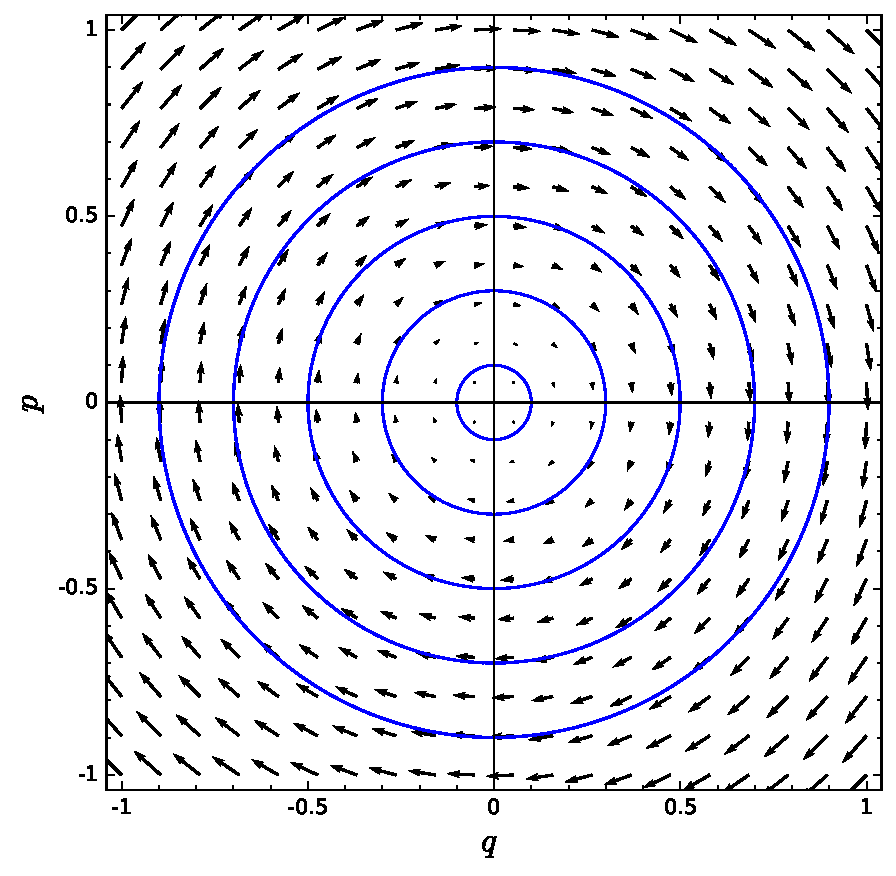
\includegraphics[width=0.4\textwidth]{pics/oscilador}
    \label{fig:oscilador}
    \caption{\small Espacio de fases del oscilador armónico junto al campo y a las curvas de energía constante. En este caso $k=m=1$, de modo que las curvas de energía constante son circunferencias de radio $\sqrt{2E}$.}
  \end{figure}

  Ahora, si tomamos unas coordenadas «polares» $(E,\phi)$, donde $\phi$ es la coordenada angular en cada una de estas elipses, la dinámica del sistema queda mucho más simplificada: 
  \begin{equation*}
    \begin{cases}
    E(t)&=E(0) \\
    \phi(t)&=\phi(0)-\omega t.
  \end{cases}
  \end{equation*}
  Sin embargo, ¿será canónica la transformación $(q,p) \rightarrow (E,\phi)$? Para ello, veamos cómo se comporta la forma $\Omega_1=\dd p\wedge \dd q$ con el cambio
  \begin{equation*}
    \begin{cases}
      q(E,\phi)=\sqrt{\frac{2E}{k}}\cos\phi\\
      p(E,\phi)=\sqrt{2mE}\sin \phi.
    \end{cases}
  \end{equation*}
  Tenemos entonces
  \begin{equation*}
    \begin{cases}
      \dd q= \frac{1}{\sqrt{2kE}}\cos \phi \dd E - \sqrt{\frac{2E}{k}} \sin \phi \dd \phi \\
      \dd p= \sqrt{\frac{m}{2E}}\sin \phi \dd E + \sqrt{2mE} \cos \phi \dd \phi,
    \end{cases}
  \end{equation*}
  y 
  \begin{equation*}
    \Omega_1= \dd p \wedge \dd q = -\sqrt{\tfrac{m}{k}}(\cos^2 \phi + \sin^2 \phi) \dd E \wedge \dd \phi= -\tfrac{1}{\omega} \dd E \wedge \dd \phi.
  \end{equation*}
  Por tanto, si definimos la \emph{variable de acción}, $J=-\frac{E}{\omega}$, entonces $\Omega_1=\dd J \wedge \dd \phi$ y $(J,\phi)$ son unas coordenadas de Darboux.

  Para tratar de dar sentido físico a esta variable $J$, consideremos el área $A_E$ de la región $S_E$ encerrada por la curva de energía constante $M_E$. Por la fórmula del área de la elipse
  \begin{equation*}
    A_E=\pi \sqrt{2mE} \sqrt{\frac{2E}{k}}=2\pi \sqrt{\frac{m}{k}} E= 2 \pi \frac{E}{\omega}= -2\pi J.
  \end{equation*}

  Observemos ahora que como $\Omega_1$ es la forma de área en $\RR^2$, 
  \begin{equation*}
    A_E=\int_{S_E}\Omega_1 = \int_{S_E} \dd p \wedge \dd q = \int_{M_E}p\dd q,
\end{equation*}
donde hemos usado el teorema de Stokes y el hecho de que $\dd p \wedge \dd q= \dd(p\dd q)$. De modo que podemos redefinir la variable de acción en la forma
\begin{equation*}
  J=-\frac{1}{2\pi}\int_{M_E}p \dd q.
\end{equation*}
Este será el aspecto que tengan las variables de acción-ángulo en general para sistemas con un grado de libertad. Regresando ahora a las coordenadas originales, tenemos
\begin{equation*}
  \begin{cases}
    q(J,\phi)=\sqrt{-\frac{2J\omega}{ k}}\cos \phi\\
    p(J,\phi)=\sqrt{-2m\omega J}\sin \phi.
  \end{cases}
\end{equation*}

\paragraph{\bf Oscilador armónico con $n$ grados de libertad}\mbox{}

  Para estudiar un caso de dimensión superior, podemos considerar el sistema formado por $n$ osciladores armónicos no acoplados o, equivalentemente, un oscilador armónico con $n$ grados de libertad. El hamiltoniano del sistema será (tomando $k=m=1$)
  \begin{equation*}
    H(q_1,\dots,q_n,p_1,\dots,p_n)= H_1(q_1,p_1)+ \cdots +H_n(q_n,p_n) = \tfrac{1}{2}\sum_{i=1}^n (p_i^2+q_i^2).
  \end{equation*}
  Este sistema es integrable en el sentido de Liouville. Basta tomar $F=(H,H_2+\cdots+H_{n},H_3+\cdots+H_{n-2},\dots,H_n)$, ya que 
  \begin{equation*}
    \pois{H_i}{H_j} = \sum_{k=1}^n\left( \parcial{H_i}{p_k}\parcial{H_j}{q_k} - \parcial{H_j}{p_k}\parcial{H_i}{q_k}\right)=0
  \end{equation*}
  y las componentes de $F$ son independientes en casi todo punto de $\RR^{2n}$. 
  
  Ahora, dado $a=(a_1,\dots,a_n)\in \RR^n$, $M_a=F^{-1}(a)$ vendrá dado por 
  \begin{equation*}
    \left\lbrace
    \begin{array}{l}
      \tfrac{1}{2}(p_1^2+q_1^2)=a_1-a_2 \\
      \tfrac{1}{2}(p_2^2+q_2^2)=a_2-a_3 \\
\vdots \\
\tfrac{1}{2}(p_n^2+q_n^2)=a_n, 
    \end{array}
    \right.
  \end{equation*}
  que son las ecuaciones de un toro $n$-dimensional. Cada una de las ecuaciones $\frac{1}{2}(p_i^2+q_i^2)=a_i-a_{i+1}$ da una circunferencia $C_{a,i}$ de radio $r_i=\sqrt{2(a_i-a_{i+1}}$, de modo que $M_a=C_{a,1}\times\dots\times C_{a,n}$. Nótese que en este caso los valores críticos son precisamente aquellos $a$ con varias componentes iguales, de forma que los puntos críticos formarán toros de dimensión menor.

  Consideremos $\gamma_{a,i}$ lazos en cada circunferencia $C_{a,i}$, de manera que los $\gamma_{a,i}$ son generadores del grupo fundamental de $M_a$. Entonces podemos definir las variables de acción 
  \begin{equation*}
    J_i(a) = \frac{1}{2\pi}\int_{\gamma_{a,i}} \sum_{k=1}^n p_k \dd q_k.
  \end{equation*}
  La definición de estas variables no depende de la base elegida ya que, por el teorema de Stokes,
  \begin{equation*}
    \int_{\gamma_{i,a}} \sum_{k=1}^n p_k \dd q_k- \int_{\gamma_{i,a}'} \sum_{k=1}^n p_k \dd q_k = \int_{\sigma} \omega=0,
  \end{equation*}
  donde $\sigma$ es la región encerrada por las curvas, ya que $\omega|_{M_a}=0$ y en $M_a$ no hay puntos críticos.

  Consideremos ahora las variables angulares $\phi_i$ a lo largo de cada $C_{i,a}$. Podemos tomar entonces las nuevas coordenadas $(J,\phi)$, con
  \begin{equation*}
      J_i(q,p)=J_i(F(q,p))=\frac{1}{2\pi}\int_{\gamma_{F(q,p),i}} \sum_{k=1}^n p_k \dd q_k 
  \end{equation*}
  y $\phi(q,p)$ las variables angulares en el toro $M_{F(q,p)}$.
  Si la carta $(J,\phi)$ es de Darboux, las ecuaciones de Hamilton pueden integrarse por cuadraturas. Esto se debe a que $J=J(a)$, de modo que, por las ecuaciones de Hamilton,
\begin{equation*}
  \parcial{H}{\phi_i}=-\dot{J_i}=0.
\end{equation*}
Por tanto, $H=H(J_1(a),\dots,J_n(a))$ y 
\begin{equation*}
  \dot{\phi_i}=\parcial{H}{J_i} = \omega_j(a),
\end{equation*}
con $\omega_j$ constante en $M_a$. Las ecuaciones de Hamilton quedan entonces integradas en la forma
\begin{equation*}
  \begin{cases}
  J(t)= & J(a) \\
  \phi(t) = & \phi(0) + \omega(a) t.
\end{cases}
\end{equation*}


\section{Movimiento condicionalmente periódico}\label{sec:promedios}
Una vez tenemos a nuestra disposición el teorema de Arnold-Liouville, sabemos que el flujo en los toros invariantes de los sistemas integrables en el sentido de Liouville será muy sencillo. En esta sección vamos a estudiar el flujo en estos toros y obtendremos un teorema muy importante sobre este tipo de sistemas.

  En primer lugar, consideremos un $2$-toro invariante con la dinámica del teorema (por ejemplo, el asociado a los niveles de energía de un oscilador armónico bidimensional). Sea $(\theta_1,\theta_2)$ un punto en el toro y su trayectoria bajo el flujo hamiltoniano $\gamma(t)=\varphi_t(\theta_1,\theta_2)=(\theta_1+\omega_1t,\theta_2+\omega_2t)$. Si $\omega_1/\omega_2=m/n$ es racional, entonces 
  \begin{equation*}
    \gamma\left(\frac{2n\pi}{\omega_2}\right) = (\theta_1+2m\pi,\theta_2+2n\pi)=(\theta_1,\theta_2).
  \end{equation*}
  Es decir, a cierto tiempo la trayectoria «se cierra». Estas órbitas se dicen \emph{periódicas}. 
 
  Sin embargo, si $\omega_2/\omega_1$ es irracional, dado un ángulo $\alpha$ y sea $T$ tal que $\alpha=\theta_1+\omega T$, entonces, sea $T_n=T+2n\pi/\omega_1$, $\alpha=\theta_1+\omega_1(T_n)$ para cada $n\in \NN$. Ahora, la aplicación
  \begin{equation*}
    \begin{array}{rcl}
    g:\SF^1 & \longrightarrow &\SF^1 \\
  \phi & \longmapsto & \phi + 2\pi\frac{\omega_2}{\omega_1},
  \end{array}
\end{equation*}
es una rotación de ángulo un múltiplo irracional de $2\pi$ en la circunferencia del toro de ángulo $\alpha$. Entonces, como ya vimos por el teorema de recurrencia de Poincaré, $\{g^n(\phi)|n\in \NN\}$ es denso en $\SF^1$. Como esto es válido para todo $\alpha$ y se cumple 
\begin{equation*}
  \gamma(T_n)=(\alpha,g^n(\theta_2)+\omega_2 T),
\end{equation*}
tenemos que $\{\gamma(t)|t \in \RR \}$ es denso en el toro. Este tipo de órbitas se llaman \emph{cuasiperiódicas}. Una forma sencilla de visualizar esto es mediante las \emph{figuras de Lissajous} 
\begin{equation*}
  L_{\omega}=\{(\cos t, \cos \omega t) | t \in \RR\},
\end{equation*}
ver figura \ref{fig:lissajous}.
\begin{figure}[h!]
  \centering
  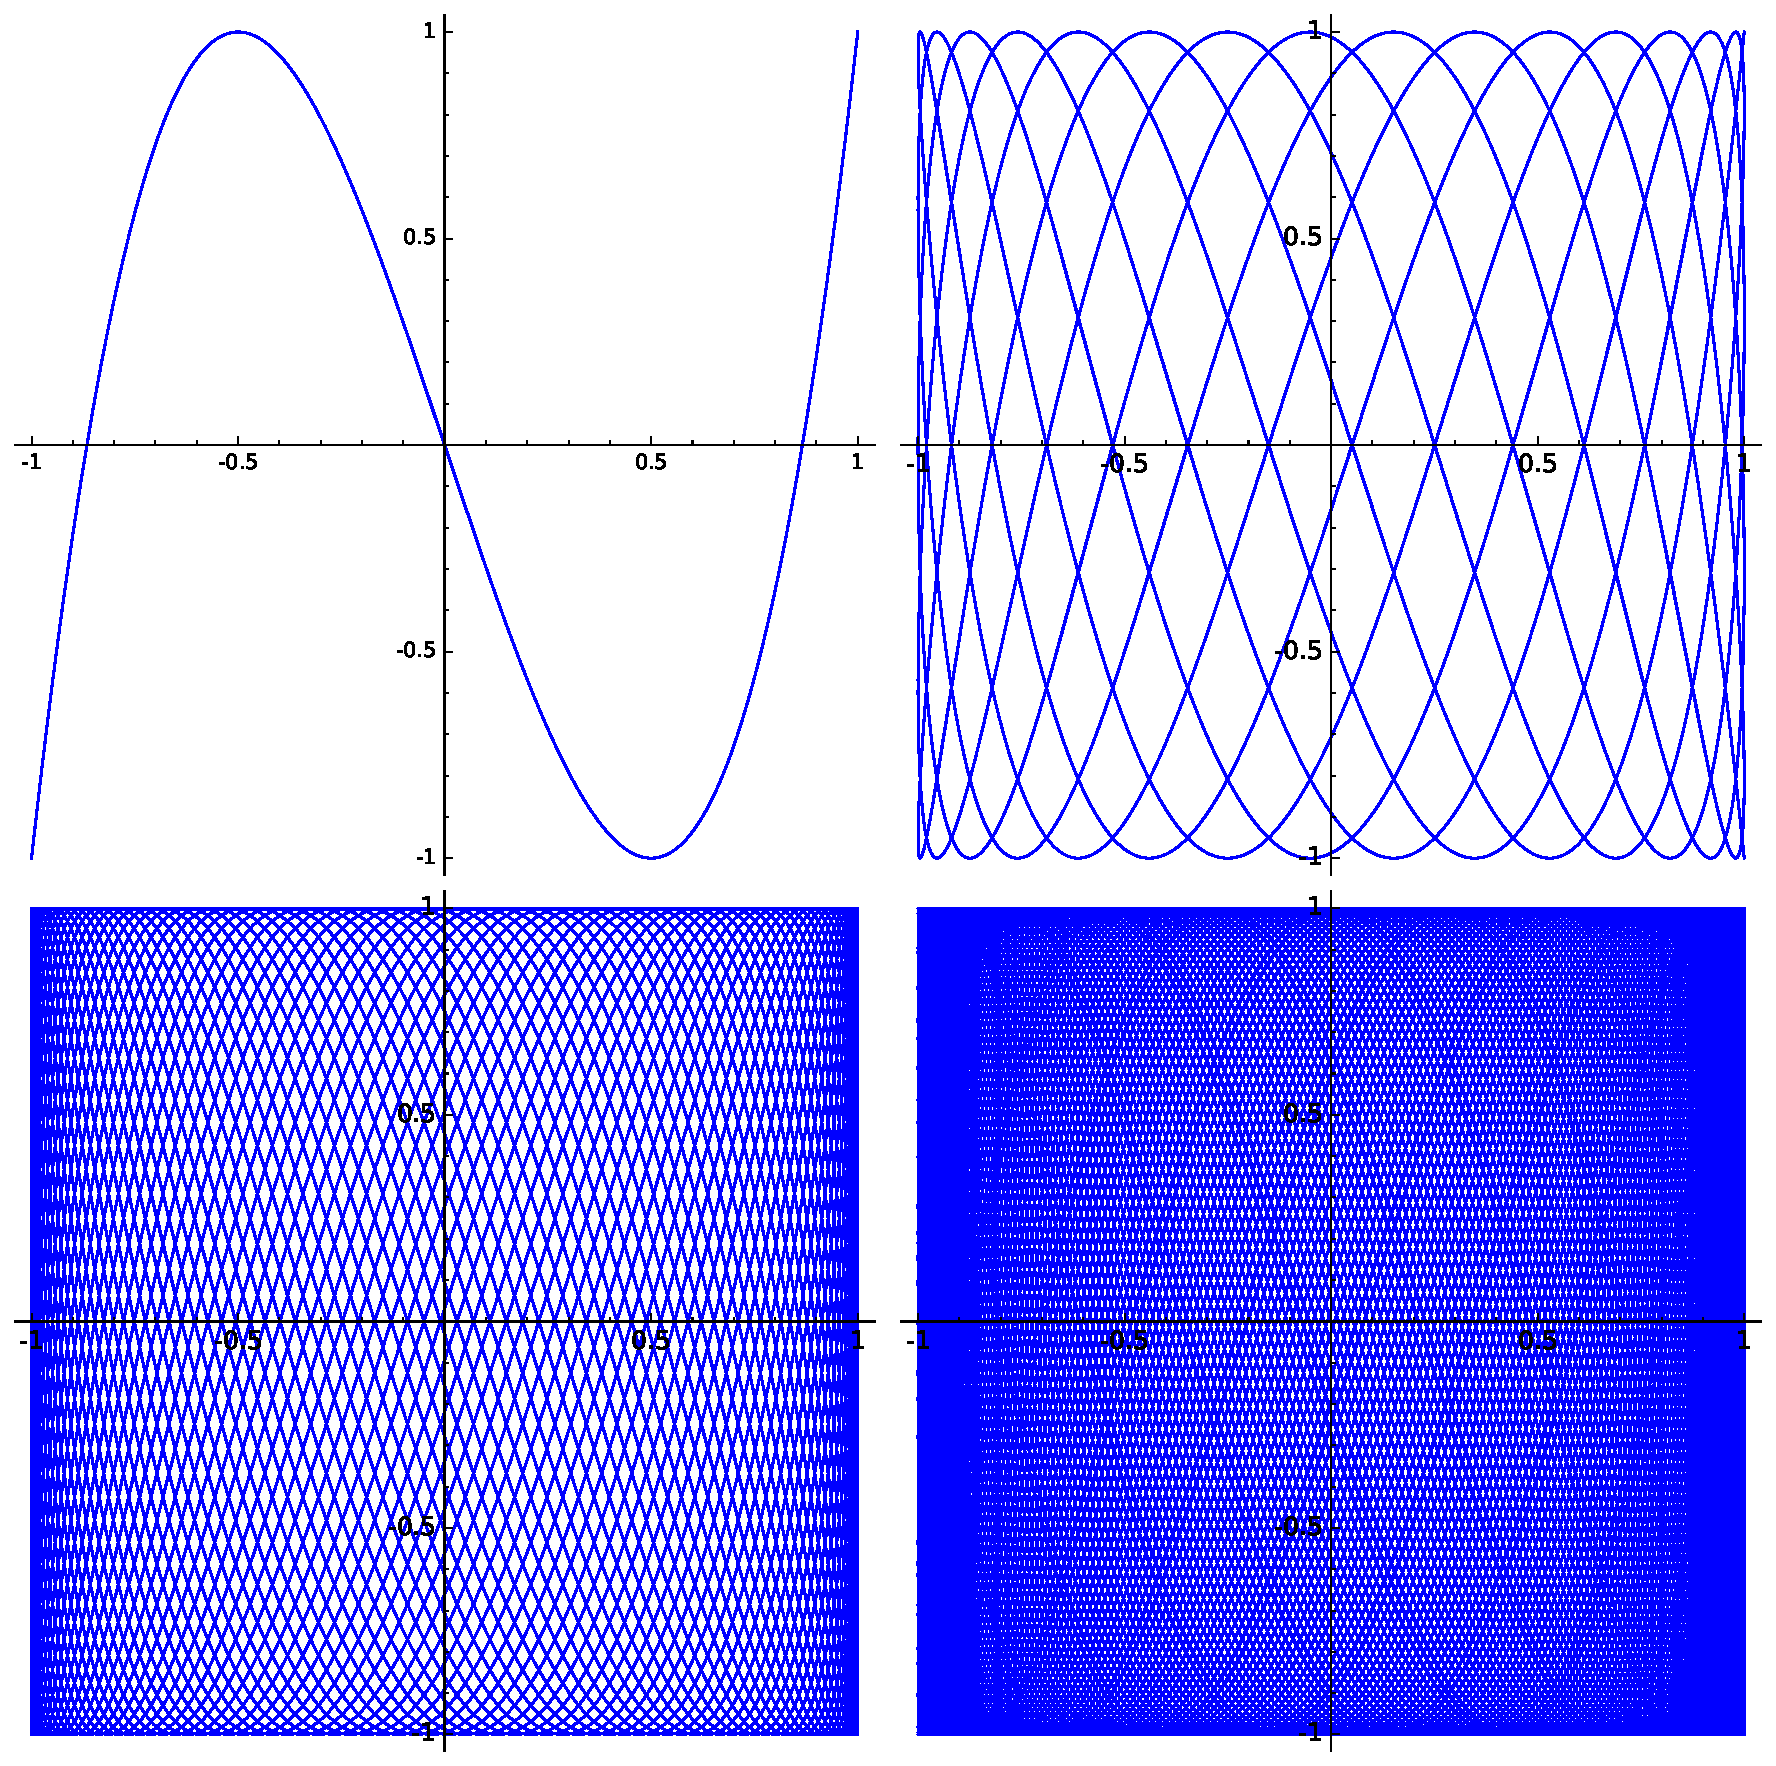
\includegraphics[width=0.6\textwidth]{pics/lissajous}
  \caption{\small Figuras de Lissajous para $\omega=3,$ $3.1,$ $3.14,$  y $3.1416$, $t \in (0,128\pi)$ con pasos de $0.01$.}
  \label{fig:lissajous}
\end{figure}

Vamos a generalizar ahora estas ideas al caso $n$-dimensional.

\begin{defn}[Movimiento condicionalmente periódico en $\TT^n$]
  \em
  Sean $\TT^n$ el toro n-dimensional y $\phi=(\phi_1,\dots,\phi_n)$ coordenadas angulares. Se entiende por un \emph{movimiento condicionalmente periódico} en el toro el flujo uniparamétrico dado por 
  \begin{equation*}
    \phi(t)=\phi(0)+\omega t
  \end{equation*}
  con $\omega=(\omega_1,\dots,\omega_n)$ \emph{frecuencias} constantes en el toro. Las frecuencias $\omega$ se dicen \emph{independientes} si, sea $k \in \ZZ^n$, entonces $\esc{k}{\omega}=0$ si y sólo si $k=0$.
\end{defn}
\begin{defn}[Promedios espacial y temporal]
  \em
  Sea $f:\TT^n \rightarrow \RR$ una función integrable Riemann,
  \begin{enumerate}
    \item El \emph{promedio espacial} de $f$ en $\TT^n$ es el número
      \begin{equation*}
	\bar{f}=\frac{1}{(2\pi)^n}\int_0^{2\pi} \cdots \int_0^{2\pi} f(\phi) d\phi_1,\dots,d\phi_n.
      \end{equation*}
    \item El \emph{promedio temporal} de $f$ en $\TT^n$ es la función
      \begin{equation*}
	f^*(\phi_0)=\lim_{T\rightarrow \infty} \int_0^{T}f(\phi_0+\omega t) dt,
      \end{equation*}
      definida en los puntos $\phi_0$ en los que exista el límite.
  \end{enumerate}
\end{defn}

\begin{thm}[Teorema de los promedios]
  Si $f:\TT^n \rightarrow \RR$ es una función integrable Riemann y las frecuencias $\omega$ son independientes, el promedio temporal está bien definido en todo el toro $\TT^n$ y coincide en todo punto con el promedio espacial.
\end{thm}
\begin{proof}
    En primer lugar, consideramos funciones de la forma $e^{i\esc{k}{\phi}}$, $k\in \ZZ^n$. Si $k=0$, entonces $\bar{f}=f=f^*=1$. Si $k\neq0$, $\bar{f}$ es una integral a periodos en funciones trigonométricas, luego es igual a 0. Por otra parte
     \begin{equation*}
       \int_0^T e^{i\esc{k}{\phi_0 + \omega t}} dt= e^{i\esc{k}{\phi_0}}\int_0^T e^{i\esc{k}{\omega}t}dt=e^{i\esc{k}{\phi_0}}\frac{e^{i\esc{k}{\omega}T}-1}{i \esc{k}{\omega}}.
     \end{equation*}
     Por tanto, el promedio temporal será
     \begin{equation*}
       \lim_{T\rightarrow \infty}\frac{e^{i\esc{k}{\phi_0}}}{i \esc{k}{\omega}}\frac{e^{i\esc{k}{\omega}T}-1}{T}=0.
     \end{equation*}
     
    Como los promedios dependen linealmente de $f$, también coincidirán para los polinomios trigonométricos
     \begin{equation*}
       f=\sum_{|k|<N}f_ke^{i\esc{k}{\omega}}.
     \end{equation*}

    Dado $\varepsilon >0$, si $f$ es continua y real por el teorema de Weierstrass podemos aproximarla por un polinomio trigonométrico $P$ que cumpla $|f-P|<\frac{1}{2}\varepsilon$. Sean $P_1=P-\frac{1}{2}\varepsilon$, $P_2=P+\frac{1}{2}\varepsilon$ entonces
     \begin{equation*}
       \bar{P_2}-\bar{P_1}=\frac{1}{(2\pi)^n}\int_{\TT^n} (P_2 - P_1) d\phi = \frac{1}{(2\pi)^n}\varepsilon (2\pi)^n= \varepsilon.
     \end{equation*}

    Dado $\varepsilon >0$, si $f$ es real e integrable Riemann, entonces existen dos funciones continuas $f_1,f_2$ tales que $f_1<f<f_2$ y $\int_{\TT^n}\frac{1}{(2\pi)^n}(f_2-f_1)d\phi<\frac{1}{3}\varepsilon$. Tomando ahora $P_1,P_2$ polinomios trigonométricos tales que $P_1<f_1<f_2<P_2$ y $\int_{\TT^n}\frac{1}{(2\pi)^n}(P_i-f_i)d\phi < \frac{1}{3}\varepsilon$, para $i=1,2$, entonces
     \begin{equation*}
       \bar{P_2}-\bar{P_1}=\frac{1}{(2\pi)^n}\int_{\TT^n} (P_2 - P_1) d\phi = \frac{1}{(2\pi)^n}\varepsilon (2\pi)^n= \varepsilon.
     \end{equation*}

    Por último, sea $\varepsilon>0$, entonces existen dos polinomios trigonométricos $P_1,P_2$ tales que $P_1<f<P_2$ y $\bar{P_2}-\bar{P_1}<\varepsilon$. Ahora, como $f<P_2$,
     \begin{equation*}
       \frac{1}{T}\int_0^T f(\phi(t))dt < \frac{1}{T}\int_0^T P_2(\phi(t))dt,
     \end{equation*}
     luego
     \begin{equation*}
       \left| \frac{1}{T}\int_0^T f(\phi(t))dt- \bar{f} \right| <\left| \frac{1}{T}\int_0^T P_2(\phi(t))dt- \bar{f} \right| < \left| \frac{1}{T}\int_0^T P_2(\phi(t))dt- \bar{P_2}\right| + |\bar{P_2}-\bar{f}|.
     \end{equation*}
     Pero, como $P_1<f<P_2$, por la monotonía de la integral $\bar{P_1}<f<\bar{P_2}$, luego $|\bar{P_2}-\bar{f}|<|\bar{P_2}-\bar{P_1}|<\varepsilon$. Además, como $P_2$ es un polinomio trigonométrico existe un $T_0$ tal que, si $T>T_0$
     \begin{equation*}
       \left| \frac{1}{T}\int_0^T P_2(\phi(t))dt- \bar{P_2}\right| < \varepsilon .
     \end{equation*}
     Finalmente, obtenemos lo que queríamos probar
     \begin{equation*}
       \left| \frac{1}{T}\int_0^T f(\phi(t))dt- \bar{f} \right| <\left| \frac{1}{T}\int_0^T P_2(\phi(t))dt- \bar{P_2}\right| + |\bar{P_2}-\bar{f}|<\varepsilon + \varepsilon = 2\varepsilon,
     \end{equation*}
     luego $f^*(\phi_0)=\lim_{t\rightarrow \infty}\frac{1}{T}\int_0^T f(\phi(t)) dt = \bar{f}$.
\end{proof}
\begin{corol}
  Si las frecuencias son independientes, entonces, para todo $\phi_0 \in \TT^n$, \[\{\phi(t)=\phi_0+\omega t|t\in \RR\}\] es denso en el toro $\TT^n$.
\end{corol}
\begin{proof}
  En caso contrario, podemos tomar un abierto $D$ del toro que no tiene ningún punto de la trayectoria $\phi(t)$. Construimos la función 
  \begin{equation*}
    f(\phi)=\left\lbrace
    \begin{array}{ll}
      0 & \text{si } \phi \not\in D \\
      \frac{(2\pi)^n}{\int_D d\phi} & \text{si } \phi \in D.
    \end{array}
    \right.
  \end{equation*}
  Claramente, $\bar{f}=1$, pero $f^*(\phi_0)=0$, lo que contradice el teorema de los promedios.
\end{proof}
\begin{corol}
  Sea $D\subset \TT^n$ un conjunto medible Jordan. Sea $A_D=\{t\in \RR | \phi(t) \in D\}$ (que también es medible Jordan) y sea $\tau_D(T)=\int_0^T\chi_{A_D}(t)dt$. Entonces
  \begin{equation*}
    \lim_{T\rightarrow \infty}\frac{\tau_D(T)}{T}= \frac{\mathrm{Vol}(D)}{(2\pi)^n}.
  \end{equation*}
\end{corol}
\begin{proof}
  Aplicamos el teorema a $\chi_D$, entonces $\int_0^T \chi_D(\phi(t))dt=\int_0^T \chi_{A_D}(t)dt=\tau_D(t)$ y $\bar{\chi}_D=(2\pi)^{-n}\mathrm{Vol}(D)$. Finalmente, por el teorema de los promedios
  \begin{equation*}
    \bar{\chi}_D=\frac{\mathrm{Vol}(D)}{(2\pi)^n}=\lim_{T\rightarrow \infty}\frac{1}{T}\int_0^T \chi_D(\phi(t))dt=\lim_{T\rightarrow \infty}\frac{\tau_D(T)}{T}.
  \end{equation*}
\end{proof}

\section{Sistemas con un grado de libertad}
En esta sección damos algunas generalidades sobre los sistemas hamiltonianos con un grado de libertad que, como ya hemos visto, son todos integrables en el sentido de Liouville. Uno de los ejemplos más característicos es el péndulo simple, que estudiamos a continuación.
  
\paragraph{\bf El péndulo simple}\mbox{}
  
  Consideramos un péndulo de masa $m=1$ cuya «cuerda» es una barra rígida de masa despreciable y longitud $1$. El espacio de configuración del péndulo es entonces la circunferencia unidad $\SF^1$ y su espacio de fases será el fibrado tangente de $\SF^1$, que no es otra cosa que un cilindro. Tomando como coordenada generalizada el ángulo $\phi$ de desviación del péndulo respecto de la vertical, el hamiltoniano viene dado por 
  \begin{equation*}
    H(\phi,p)=\frac{1}{2}p^2 - g\cos\phi,
  \end{equation*}
  donde $g$ es la aceleración de la gravedad y hemos tomado el centro como origen de energía potencial.
  \begin{figure}[h]
    \centering
    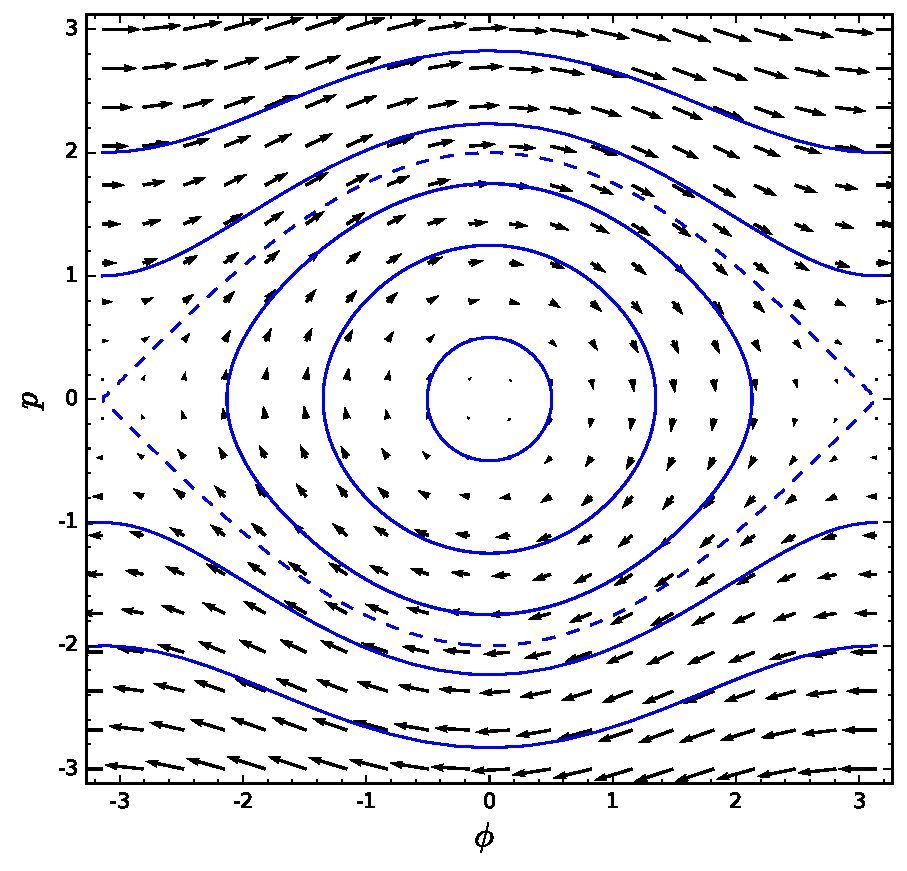
\includegraphics[width=0.4\textwidth]{pics/pendulo}
    \label{fig:pendulo}
    \caption{\small Espacio de fases del péndulo junto al campo hamiltoniano y las curvas de nivel. Nótese que el lado derecho ($\phi=\pi$) está identificado con el lado izquierdo ($\phi=-\pi$), ya que se trata de un cilindro.}
  \end{figure}
  Como podemos ver en la figura \ref{fig:pendulo}  las trayectorias son cerradas, luego cada curva de energía constante es compacta. Para estudiar los puntos críticos, nótese que $\dd H$ es distinta de 0 en todo punto exceptuando los casos $(\phi=0,p=0)$ y $(\phi=\pi,p=0)$, que corresponden a puntos de equilibrio (el primero, estable, el segundo, inestable) donde la trayectoria es sólo un punto. La curva que aparece punteada en la figura, de ecuación
  \begin{equation*}
    g=H(\phi,p)=\frac{1}{2}p^2 - g \cos\phi ,
  \end{equation*}
   corresponde al punto de equilibrio y a dos trayectorias que tienden asintóticamente al punto de equilibrio inestable. Este conjunto no es un toro de Liouville ya que contiene al punto crítico $(\pi,0)$. Estas trayectorias son matemáticamente factibles aunque su realización práctica parezca una tarea imposible. Las curvas que quedan dentro de la curva punteada corresponden a movimientos de oscilación en torno al punto de equilibrio estable, mientras que las que quedan fuera corresponden a movimientos de rotación del péndulo alrededor de su centro. 

   \paragraph{\bf Puntos críticos de los sistemas con un grado de libertad}\mbox{}

   Los dos tipos de punto crítico que presenta el péndulo simple se conocen como \emph{centros}, para el $(0,0)$ y \emph{sillas}, para el $(\pi,0)$. Podemos probar que, de hecho esos son los únicos tipos de punto crítico que puede presentar un sistema hamiltoniano en $\RR^2$. En efecto, supongamos que $(0,0)$ es un punto de equilibrio de un sistema hamiltoniano. Podemos escribir las ecuaciones de Hamilton en la forma
   \begin{equation*}
     \left(
     \begin{array}{c}
       \dot q \\
       \dot p
     \end{array}
     \right)=
\left(
     \begin{array}{cc}
       0 & -1\\
       1 & 0
     \end{array}
     \right)
\left(
     \begin{array}{c}
       \parcial{H}{q} \\
       \parcial{H}{p},
     \end{array}
     \right)
   \end{equation*}
   de modo que su versión linealizada en torno al $(0,0)$ será
   \begin{equation*}
     \left(
     \begin{array}{c}
       \dot q \\
       \dot p
     \end{array}
     \right)=
\left(
     \begin{array}{cc}
       0 & -1\\
       1 & 0
     \end{array}
     \right)
     \left.
\left(
     \begin{array}{cc}
       \frac{\partial^2 H}{\partial q^2} & \frac{\partial^2 H}{\partial p \partial q} \\
       \frac{\partial^2 H}{\partial q \partial p} & \frac{\partial^2 H}{\partial p \partial p} 
     \end{array}
     \right)
     \right|_{(q,p)=(0,0)}
\left(
     \begin{array}{c}
       q \\
       p
     \end{array}
     \right)
     =J_1 B
\left(
     \begin{array}{c}
       q \\
       p
     \end{array}
     \right)
     =A
\left(
     \begin{array}{c}
       q \\
       p
     \end{array}
     \right).
   \end{equation*}
   De la simetría de la matriz de segundas derivadas $B$ y de las propiedades de la matriz $J_1$, tenemos que $A$ ha de cumplir la condición
   \begin{equation*}
     A^{t}J_1+J_1 A=0.
   \end{equation*}
   Las matrices que cumplen esta condición forman el álgebra de Lie $\mathfrak{sp}(2)$ del grupo simpléctico $\mathrm{Sp}(2)$.

   Ahora, se tiene la siguiente proposición.
   \begin{prop}
     Si $\alpha$ es un autovalor de una matriz $A\in \mathfrak{sp}(2)$ con multiplicidad algebraica $k$, entonces $-\alpha$ es también un autovalor de $A$ con la misma multiplicidad. Si $\alpha=0$ entonces su multiplicidad es par.
   \end{prop}
   \begin{proof}
     Los autovalores son los ceros del polinomio característico $P(\alpha)=\det(\alpha I-A)$. Por tanto, basta probar que $\det(\alpha I-A)=\det(\alpha I + A)$. Esto se ve de la siguiente manera,
     \begin{align*}
       P(\alpha)&=\det(\alpha I-A)=\det(-\alpha J_1^2-J_1B)=\det J_1\det(-\alpha J_1 - B)\\
       &=\det(-\alpha J_1-B)^t=\det (\alpha J_1 - B)=\det(\alpha I - J_1^{-1}B)\\
       &=\det(\alpha I + J_1 B)=\det(\alpha I +A).
     \end{align*}
   \end{proof}
   Por tanto, los autovalores de $A$ son imaginarios, opuestos o ambos cero, luego el punto crítico $(0,0)$ solo puede ser un centro (en el caso de autovalores imaginarios) o un punto de silla (en el caso de autovalores reales opuestos). Como consecuencia de esto tenemos que el sistema hamiltoniano no puede tener puntos \emph{asintóticamente estables}, lo que tal vez era de esperar a la vista de la conservación de la energía y del teorema de Liouville: los puntos asintóticamente estables funcionarían como «fuentes» o «sumideros» del área de Liouville.



   \section{Más sistemas integrables}
   Cuando estudiamos sistemas con varios grados de libertad, la integrabilidad requiere de la existencia de cantidades conservadas adicionales. Como ya vimos en el apartado de simetrías y leyes de conservación, una forma útil de encontrar cantidades conservadas es observar las simetrías del sistema, siguiendo el mecanismo de Noether. En esta sección veremos dos ejemplos donde podemos ver directamente esta relación entre las simetrías y la integrabilidad del sistema.

   \paragraph{\bf El péndulo esférico}\mbox{}

   Un péndulo esférico consiste en una partícula (aquí supondremos de masa $m=1$) enganchada por una barra rígida de masa despreciable y de longitud 1 a un punto del espacio y bajo la acción de la gravedad. Es decir, es como un péndulo simple, solo que no está restringido a oscilar en un solo plano, sino que puede moverse libremente, ver figura \ref{fig:espendulo}.
\begin{figure}[h]
  \centering
  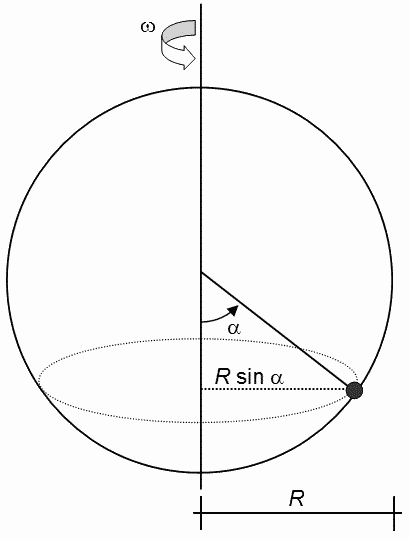
\includegraphics[width=0.3\textwidth]{pics/espendulo.png}
  \caption{\small Péndulo esférico}
  \label{fig:espendulo}
\end{figure}

Podemos considerar el sistema inmerso en $\RR^3$, de modo que el espacio de fases en principio será el espacio simpléctico estándar $6$-dimensional $(\RR^6,\Omega_3)$. Ahora, la ligadura del péndulo restringe el movimiento espacial a una esfera de radio 1, y las velocidades serán siempre tangentes a esta esfera. De este modo, el espacio de fases será
\begin{equation*}
  M=\left\{ (q,p)\in \RR^6 : ||q||=1, \esc{q}{p}=0 \right\},
\end{equation*}
que claramente es difeomorfo al fibrado tangente de la esfera, $T\SF^2$. La forma simpléctica en $M$ será simplemente la restricción de $\Omega_3$ a $M$. El hamiltoniano será la restricción a $M$ de la función 
\begin{align*}
  H :\RR^6&\longrightarrow \RR\\ 
  (q,p) &\longmapsto \tfrac{1}{2m}||p||^2+mgq_3, 
  \end{align*}
  donde $q_3$ es la componente vertical del vector $q=(q_1,q_2,q_3)$.

  Observemos ahora que el sistema es invariante bajo las rotaciones en torno a la vertical. En efecto, si $R\in\mathrm{SO}(3)$ es una rotación en torno a la vertical, como la tercera componente no varía respecto de las rotaciones en torno a la vertical y las rotaciones preservan la norma,
  \begin{equation*}
    H(R(q),R(p))=\tfrac{1}{2m}||R(p)||^2+mgq_3=\tfrac{1}{2m}||p||^2+mgq_3=H(q,p).
  \end{equation*}
  Por tanto, la tercera componente del momento angular $L_3=q_1p_2-q_2p_1$ es una cantidad conservada del sistema $(M,H)$. Como $\dim(M)=4$ y hemos encontrado una cantidad conservada del sistema a parte del propio hamiltoniano, no es difícil comprobar que $H$ y $L_3$ son independientes para casi todo punto, luego el sistema $(M,H)$ será integrable en el sentido de Liouville.

  \paragraph{\bf El potencial central}\mbox{}

  Consideremos el caso genérico de una partícula moviéndose en el espacio sujeta a una fuerza central, es decir, dirigida siempre hacia el origen y cuyo valor dependa solo de la distancia de la partícula a este. Un ejemplo típico sería el de una partícula moviéndose en un potencial kepleriano ($V(r)=-k/r$) (por ejemplo, la Tierra alrededor del Sol) o en un potencial coulombiano (por ejemplo, un electrón que ``gira'' en torno a un núcleo atómico, despreciando toda clase de efectos cuánticos, si es que eso fuera posible). El espacio de fases del sistema es el espacio simpléctico estándar $6$-dimensional $(\RR^6,\Omega_3)$ y el hamiltoniano viene dado por la función
  \begin{equation*}
    H(q,p)=\tfrac{1}{2m}||p||^2+V(||q||).
  \end{equation*}
  Claramente, el sistema es invariante bajo rotaciones ya que, si $R\in \mathrm{SO}(3)$ es una rotación, entonces, como las rotaciones preservan la norma
  \begin{equation*}
    H(R(q),R(p))=\tfrac{1}{2m}||R(p)||^2+V(||R(q)||)=\tfrac{1}{2m}||p||^2+V(||q||)=H(q,p).
  \end{equation*}
  Como consecuencia, se conserva el momento angular $L=q\times p$. En particular, se conservarán $L^2=\esc{L}{L}$ y $L_3=q_1p_2-q_2p_1$. Ahora, si calculamos el corchete de Poisson
  \begin{equation*}
    \pois{L^2}{L_3}=\sum_{i=1}^3\pois{L_i^2}{L_3}=\sum_{i=1}^32L_i\pois{L_i}{L_3},
  \end{equation*}
  por la regla de Leibniz. Ahora, como $\pois{L_3}{L_3}=0$, tenemos 
  \begin{equation*}
    \pois{L^2}{L_3}=2L_1\pois{L_1}{L_3}+2L_2\pois{L_2}{L_3}.
  \end{equation*}
  Basta entonces hallar 
  \begin{equation*}
    \pois{L_1}{L_3}=\pois{q_2p_3-q_3p_2}{q_1p_2-q_2p_1},
  \end{equation*}
  que, usando la linealidad del corchete de Poisson y la identidad de Jacobi y teniendo en cuenta que $\pois{q_i}{q_j}=\pois{p_i}{p_j}=0$ podemos desarrollar hasta llegar a
  \begin{equation*}
    \pois{L_1}{L_3}=-p_3q_1\pois{q_2,p_2}-q_3p_1\pois{p_2}{q_2}=+p_3q_1-q_3p_1=-L_2.
  \end{equation*}
Un cálculo análogo muestra que $\pois{L_2}{L_3}=L_1$, de modo que
\begin{equation*}
  \pois{L^2}{L_3}=-2L_1L_2+2L_2L_1=0.
\end{equation*}

Por tanto, $H$, $L^2$ y $L_3$ son $3$ funciones en involución y además es posible comprobar que son independientes en casi todo punto de $\RR^6$, de modo que el sistema $(M,H)$ es integrable en el sentido de Liouville.


%\section{Teoría de Arnold-Liouville}\label{sec:arnoldliouville}
A la hora de estudiar sistemas dinámicos, una cuestión interesante a plantearse, con consecuencias prácticas y también de carácter fundamental, es si las ecuaciones del sistema podrán ser «integradas», es decir, si podrán ser resueltas mediante integrales definidas («cuadraturas») de funciones conocidas. Definimos entonces:
\begin{defn}[Ecuación integrable por cuadraturas]
  \em
  Una ecuación diferencial es \emph{integrable por cuadraturas} si es posible escribir su solución general en términos de sumas, productos, composiciones e integrales de funciones conocidas. 
\end{defn}
\begin{defn}[Sistema integrable por cuadraturas]
  \em
  Un sistema hamiltoniano $(M,H)$, es \emph{integrable por cuadraturas} si para todo punto $x\in M$ existe una carta simpléctica en torno a $x$ en la que el flujo hamiltoniano es integrable por cuadraturas.
\end{defn}
Es decir, un sistema hamiltoniano integrable por cuadraturas es aquel en el que, conocidas sus condiciones iniciales, podemos integrar las ecuaciones de Hamilton mediante manipulaciones algebraicas, cálculos de integrales definidas e inversiones de difeomorfismos.

Para estudiar la integrabilidad por cuadraturas de los sistemas hamiltonianos, serán cruciales las siguientes nociones:
\begin{defn}[Funciones en involución]
  \em
  Sea $M$ una variedad simpléctica y $F_1,\dots,F_n:M \rightarrow \RR$, decimos que $F_1,\dots,F_n$ \emph{están en involución} si, para cada $i,j=1,\dots,n$, $\pois{F_i}{F_j}=0$.
\end{defn}
\begin{defn}[Integrabilidad en el sentido de Liouville]
  \em
  Sea $(M,H)$ un sistema hamiltoniano y sea $2n=\dim(M)$, decimos que $(M,H)$ \emph{es integrable en el sentido de Liouville} si existen $F_1(=H),\dots,F_n:M \rightarrow \RR$ en involución, independientes para todo $x \in M$ (es decir, $\dd F_{1,x}\wedge \cdots \wedge \dd F_{n,x} \neq 0$) y, sea $F=(F_1,\dots,F_n)$, para todo $a \in F(M)\subset \RR^n$
  \[
    M_a=F^{-1}(a)=\{x \in M \mid F(x)=a\}
  \]
  es compacto.
\end{defn}

Como ya se habrá podido intuir, el propósito de esta sección es probar que todo sistema integrable en el sentido de Liouville es integrable por cuadraturas. El resultado original, formulado en términos de mecánica hamiltoniana clásica, se debe a Joseph Liouville en 1855, mientras que el resultado moderno junto con toda la teoría de los toros invariantes se debe a Vladimir Arnold en 1963. Por otra parte, las variables de acción-ángulo fueron introducidas originalmente por Delaunay en 1860 para estudiar el movimiento de la luna y más tarde, a principios del siglo XX, usadas por los físicos para estudiar el átomo de Bohr, siendo Schwarzschild el que acuñara esa terminología en 1916. La demostración original del teorema de las variables de acción-ángulo se atribuye a Mineur en 1936. 

En la bibliografía habitual de geometría simpléctica, la serie de teoremas y proposiciones que llevan a la demostración del resultado se suele nombrar «teorema de Arnold-Liouville». En este texto, hemos decidido decantarnos por el nombre de «teoría de Arnold-Liouville». Una discusión más extensa sobre la historia y el nombre de esta teoría puede encontrarse en las páginas 640 y 641 de \cite{spivak}.

En primer lugar, vamos a considerar un ejemplo característico que aclara alguna de las ideas detrás de esta teoría.
\begin{ejemplo}
  \em
  Consideramos el oscilador armónico unidimensional, con hamiltoniano
  \begin{equation*}
    H(q,p)=\frac{p^2}{2m}+\frac{1}{2}kq^2.
  \end{equation*}
  Por simplicidad, supondremos que la masa y la constante del muelle valen 1, de forma que $H(q,p)=\frac{1}{2}(p^2+q^2)$. Las curvas $C_E$ de energía constante en el espacio de fases $\RR^2$ son circunferencias de centro 0 y radio $a=\sqrt{2E}$, con
  \begin{equation*}
    E=\frac{1}{2}(p^2+q^2).
  \end{equation*}
  \begin{figure}[h]
    \centering
    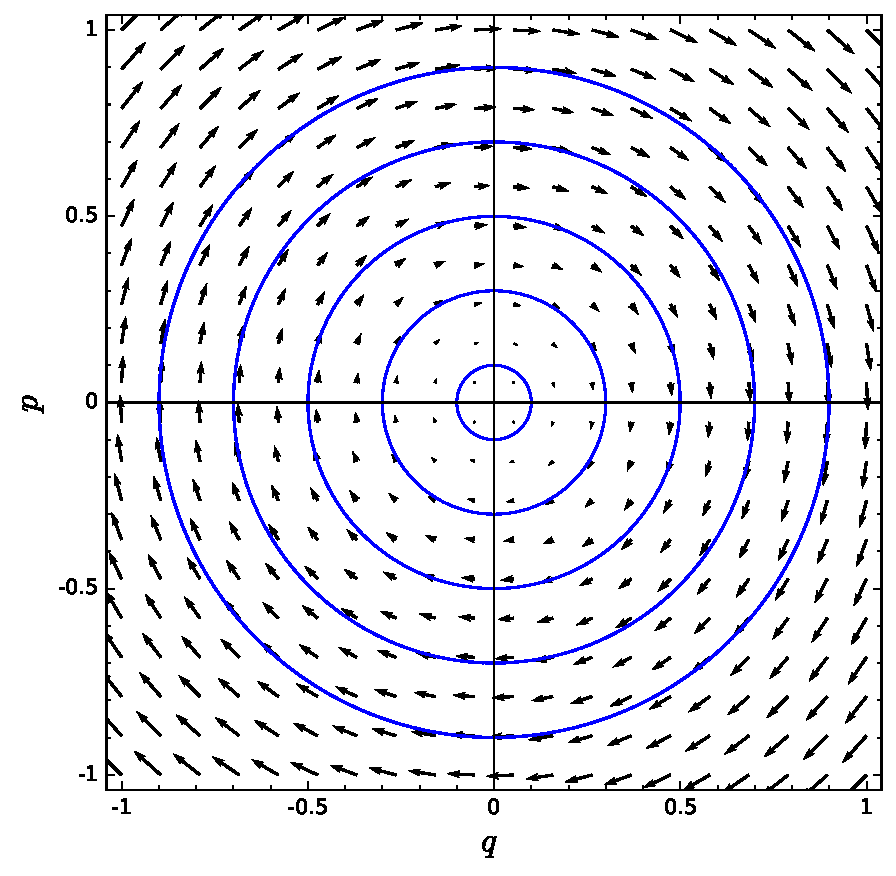
\includegraphics[width=0.4\textwidth]{pics/oscilador}
    \label{fig:oscilador}
    \caption{Espacio de fases del oscilador armónico junto al campo y al flujo hamiltonianos}
  \end{figure}
  Ahora, si tomamos unas coordenadas «polares» $(E,\phi)$, donde $\phi$ es la coordenada angular en cada una de estas circunferencias, la dinámica del sistema queda mucho más simplificada: 
  \begin{align*}
    E(t)&=E(0) \\
    \phi(t)&=\phi(0)+\omega(E(0))t.
  \end{align*}
  Sin embargo, ¿será canónica la transformación $(q,p) \rightarrow (E,\phi)$?
  \begin{figure}[h]
    \centering
    \includegraphics[width=0.6\textwidth]{pics/polar}
    \caption{Cambio de coordenadas $(q,p) \rightarrow (E,\phi)$}
    \label{fig:polar}
  \end{figure}
  En este caso es claro que la transformación preserva el área $\frac{1}{2}a^2\phi$. Más generalmente, si $A$ es una región del plano, 
  \begin{equation*}
    \text{área}(A)= \int_A r \dd r \wedge \dd \phi = \int_A \dd\left(\frac{1}{2}r^2\right) \wedge \dd \phi.
  \end{equation*}
  Por tanto, la transformación es canónica porque precisamente, si $A_E$ es la región encerrada por $C_E$, entonces
  \begin{equation*}
    E=\frac{1}{2}a^2=\frac{1}{2\pi}\text{área}(A_E).
  \end{equation*}

  En las coordenadas originales, esta área es
  \begin{equation*}
    J=\int_{A_E} \dd p \wedge \dd q = \int_{A_E}d (p\dd q) = \int_{C_E} p \dd q,
  \end{equation*}
  donde en el último paso hemos utilizado el teorema de Stokes. Esta $J$ normalmente se conoce como \emph{variable de acción}, debido a sus dimensiones.

  En un caso más general, podemos considerar el sistema formado por $n$ osciladores armónicos acoplados o, equivalentemente, un oscilador armónico $n$-dimensional. El hamiltoniano del sistema será (tomando $k=m=1$)
  \begin{equation*}
    H(q_1,\dots,q_n,p_1,\dots,p_n)= H_1(q_1,p_1)+ \cdots +H_n(q_n,p_n) = \frac{1}{2}(p_1^2+\cdots+p_n^2+q_1^2+\cdots+q_n^2).
  \end{equation*}
  Este sistema es integrable en el sentido de Liouville. Basta tomar $F=(H,H_2+\cdots+H_{n},H_3+\cdots+H_{n-2},\dots,H_n)$, ya que 
  \begin{equation*}
    \pois{H_i}{H_j} = \sum_{k=1}^n \parcial{H_i}{p_k}\parcial{H_j}{q_k} - \parcial{H_j}{p_k}\parcial{H_i}{q_k}= p_iq_j \delta_{ij} - p_jq_i \delta{ij} = p_iq_i-p_iq_i = 0,
  \end{equation*}
  y $\det(F_{*,x}) \neq 0$ para todo $x \in \RR^{2n}$. 
  
  $F^{-1}(a)$ vendrá dado por 
  \begin{equation*}
    \left\lbrace
    \begin{array}{l}
      \frac{1}{2}(p_1^2+q_1^2)=a_1-a_2 \\
      \frac{1}{2}(p_2^2+q_2^2)=a_2-a_3 \\
\vdots \\
\frac{1}{2}(p_n^2+q_n^2)=a_n, 
    \end{array}
    \right.
  \end{equation*}
  que son las ecuaciones de un toro $n$-dimensional.

  Entonces, sean $\gamma_1,\dots,\gamma_n$ una base de ciclos del toro \nota{Esto es muy intuitivo pero hay que escribirlo bien, en los libros pone que son los generadores del grupo de homología de $\TT^n$, cuando dé TOAL a lo mejor sé lo que es}, podemos definir las variables de acción 
  \begin{equation*}
    J_i = \frac{1}{2\pi}\int_{\gamma_i} \sum_{k=1}^n p_k \dd q_k = \frac{1}{2\pi} \int_{\gamma_i} \alpha.
  \end{equation*}
  La definición de estas variables no depende de la base elegida ya que, por el teorema de Stokes,
  \begin{equation*}
    \int_{\gamma_i} \alpha - \int_{\gamma_i'} \alpha = \int_{\sigma} \omega=0,
  \end{equation*}
  donde $\sigma$ es la región encerrada por las curvas y $\omega=0$ en el toro (el cálculo de esto está hecho con precisión más adelante).

Sean las variables angulares $\phi_i$ a lo largo de cada ciclo generado por $\gamma_i$, si $(q,p) \rightarrow (J,\phi)$ es canónica, podemos tomar las variables $(J,\phi)$ en las que la dinámica toma una forma especialmente simple. Esto se debe a que $J=J(a)$, de modo que, por las ecuaciones de Hamilton, 
\begin{equation*}
  \parcial{H}{\phi_i}=-\dot{J_i}=0.
\end{equation*}
Por tanto, $H=H(J_1(a),\dots,J_n(a))$ y 
\begin{equation*}
  \dot{\phi_i}=\parcial{H}{J_i} = \omega_j(a),
\end{equation*}
con $\omega_j$ constante en $M_a$. Las ecuaciones de Hamilton quedan entonces integradas en la forma
\begin{align*}
  J(t)= & J(a) \\
  \phi(t) = & \phi(0) + \omega(a) t.
\end{align*}

No hemos demostrado que el cambio de coordenadas sea un simplectomorfismo, lo que puede hacerse usando el método de Hamilton-Jacobi, que aquí no vamos a exponer. Sin embargo, no nos hará falta, ya que nosotros daremos otra prueba, demostrando un teorema general para construir variables de acción-ángulo en variedades simplécticas.
\end{ejemplo}

Vamos a estudiar también algunos ejemplos de sistemas con funciones en involución, que en ciertos supuestos serán integrables en el sentido de Liouville.
  
\begin{ejemplo}[Péndulo simple]
  \em
  Consideramos un péndulo cuya «cuerda» es una barra rígida de masa despreciable y longitud 1. El espacio de fases del péndulo es el fibrado cotangente de $\SF^1$, que no es otra cosa que un cilindro. Tomando como coordenada generalizada el ángulo $\phi$ de desviación del péndulo respecto de la vertical, el hamiltoniano viene dado por 
  \begin{equation*}
    H(\phi,p)=\frac{1}{2}p^2 - g\cos\phi,
  \end{equation*}
  donde $g$ es la aceleración de la gravedad y hemos tomado el centro como origen de energía potencial.
  \begin{figure}[h]
    \centering
    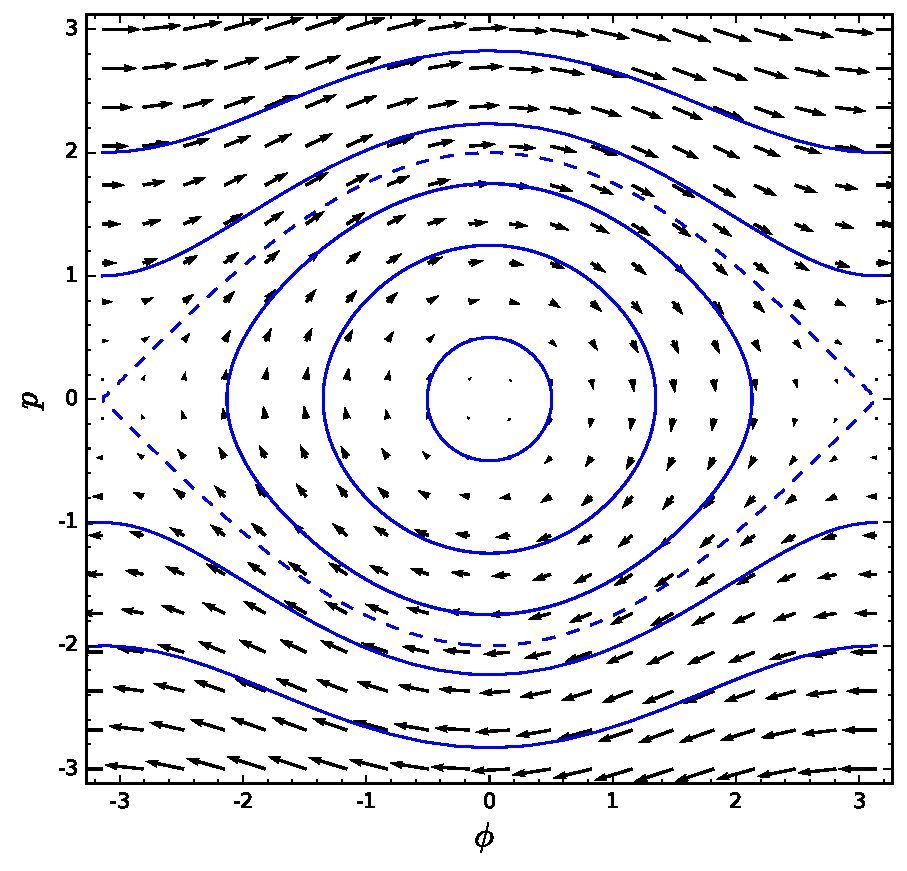
\includegraphics[width=0.4\textwidth]{pics/pendulo}
    \label{fig:pendulo}
    \caption{Espacio de fases del péndulo junto al campo y al flujo hamiltonianos.}
  \end{figure}
  Como podemos ver en la figura \ref{fig:pendulo}  las trayectorias son cerradas, luego cada curva de energía constante es compacta. $\dd H$ será distinta de 0 en todo punto exceptuando los casos $(\phi=0,p=0)$ y $(\phi=\pi,p=0)$, que corresponden a puntos de equilibrio (el primero, estable, el segundo, inestable) donde la trayectoria es sólo un punto. La curva que aparece punteada en la figura \ref{fig:pendulo}, de ecuación
  \begin{equation*}
    g=H(\phi,p)=\frac{1}{2}p^2 - g \cos\phi ,
  \end{equation*}
  corresponde al punto de equilibrio y a dos trayectorias que tienden asintóticamente al punto de equilibrio inestable. Estas trayectorias son matemáticamente factibles aunque su realización práctica parezca una tarea imposible y en ellas no aplica la teoría de Arnold-Liouville, puesto que la curva punteada no es una variedad, al contener un punto con $\dd H=0$. Estas trayectorias se conocen como \emph{singularidades} del sistema. Las curvas que quedan dentro de la curva punteada corresponden a movimientos de oscilación en torno al punto de equilibrio estable, mientras que las que quedan fuera corresponden a movimientos de rotación del péndulo alrededor de su centro. 
\end{ejemplo}
\begin{ejemplo}[Potencial central]
  \em
  Consideramos una partícula que se mueve en $\RR^3$ sometida a un potencial central, esto es, una función $V$ que sólo depende de $r=||x||$. El espacio de fases es $\RR^6$ y el hamiltoniano (tomando $m=1$) viene dado por
  \begin{equation*}
    H(x,p)=\frac{p^2}{2}+V(r).   
  \end{equation*}
  Sea ahora el momento angular
  \begin{equation*}
    L=x \times p,
  \end{equation*}
  cada una de sus componentes es $L_i=\epsilon_{ijk}(x_jp_k-x_kp_j)$, donde $\epsilon_{ijk}$ es la paridad de $(i,j,k)$ como permutación de $(1,2,3)$. Podemos calcular ahora 
  \begin{equation*}
    \pois{H}{L_i}= \sum_{k=1}^3 \parcial{H}{p_k} \parcial{L_i}{x_k} - \parcial{H}{x_k} \parcial{L_i}{p_k}= -\sum_{k=1}^3 \epsilon_{ijk}\left( p_kp_j + \frac{x_kx_j}{r}V'(r) \right)=0.
  \end{equation*}
  Por tanto, $L$ es una cantidad conservada. Al ser $L$ un vector, realmente son cantidades conservadas su norma y su dirección y sentido, lo que implica que se conservan $L^2=\esc{L}{L}$ y $L_3$. Además $\pois{L^2}{L_3}=0$, lo que nos da tres funciones en involución en el sistema.
  Sin embargo, la integrabilidad en sentido de Liouville no está garantizada por los resultados que hemos probado, ya que en general las órbitas pueden ser no acotadas y las funciones no ser independientes. 
\end{ejemplo}
\begin{ejemplo}[Trompo simétrico]
  \em
  Consideremos un trompo simétrico (la clásica peonza de juguete) que gira con su punta fija en un punto. Su espacio de configuración viene dado por las posibles rotaciones de sus ejes principales de inercia ($X',Y',Z'$) respecto a los tres ejes del sistema de laboratorio (la vertical y dos ejes arbitrarios en el suelo, $X,Y,Z$). De modo que el espacio de fases del trompo simétrico es $T^*\mathrm{SO}(3)$. Sean $I_1,I_2,I_3$ los momentos de inercia del trompo, que el trompo sea \emph{simétrico} quiere decir que $I_1=I_2$ y que el centro de masas cae sobre el eje $Z'$. En este caso, tras unos cálculos se obtiene que el hamiltoniano del sistema es
  \begin{equation*}
    H(\theta,\phi,\psi,p_{\theta},p_{\phi},p_{\psi})=\frac{p_{\theta}^2}{2I_1}+\frac{(p_{\phi}-p_{\psi}\cos\theta)^2}{2I_1\sin^2\theta}+\frac{p_{\psi}^2}{2I_3}+Mgl\cos \theta,
  \end{equation*}
  donde $g$ es la aceleración de la gravedad, $M$ es la masa de la peonza, $l$ es la distancia de la punta al centro de masas, $(\theta,\phi,\psi)$ son los ángulos de Euler de la rotación de los ejes principales de inercia respecto a los del laboratorio y $(p_{\theta},p_{\phi},p_{\psi})$ son sus momentos canónicos conjugados. 
  Las frecuencias de giro de cada uno de los ángulos de Euler $\theta$, $\phi$ y $\psi$ se llaman frecuencias de \emph{nutación}, \emph{precesión} y \emph{rotación}, respectivamente.
  \begin{figure}[h]
    \label{fig:euler}
    \centering
    \begin{minipage}[b]{0.4\textwidth}
    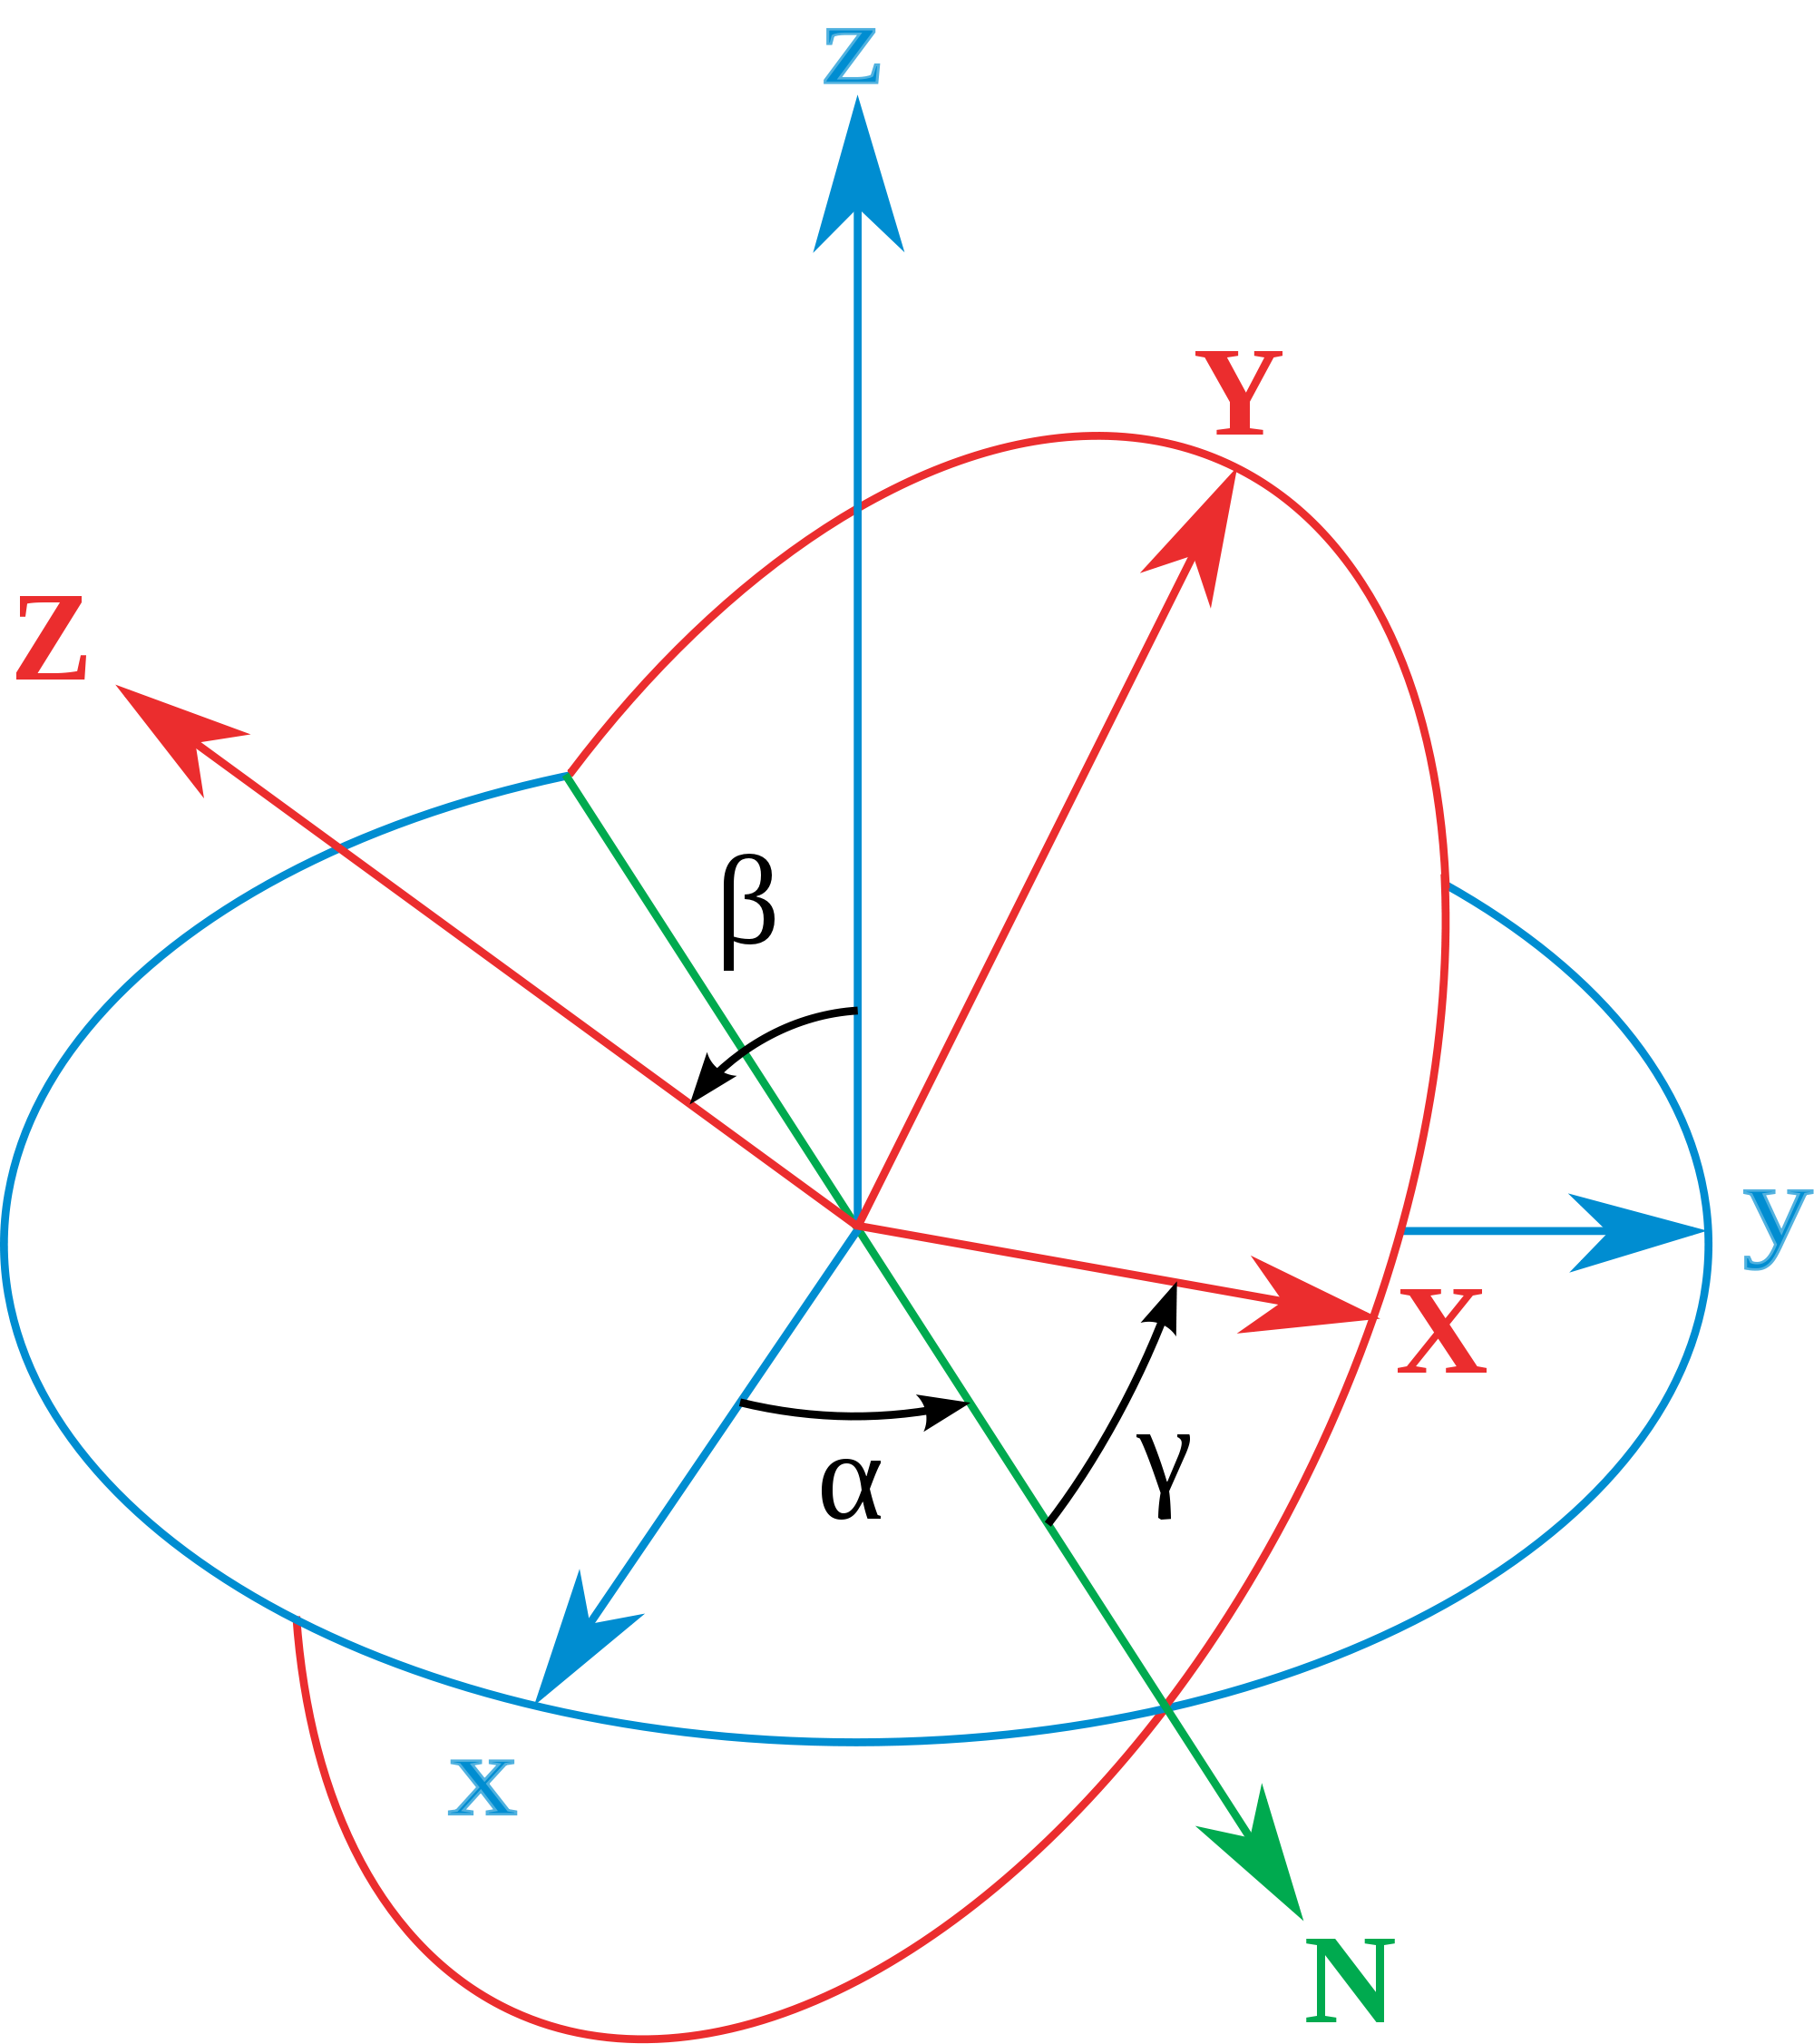
\includegraphics[width=\textwidth]{pics/euler}
    \caption{Construcción de los ángulos de Euler. Fuente: \cite{euler}.}
  \end{minipage}
  \hfill
  \begin{minipage}[b]{0.4\textwidth}
    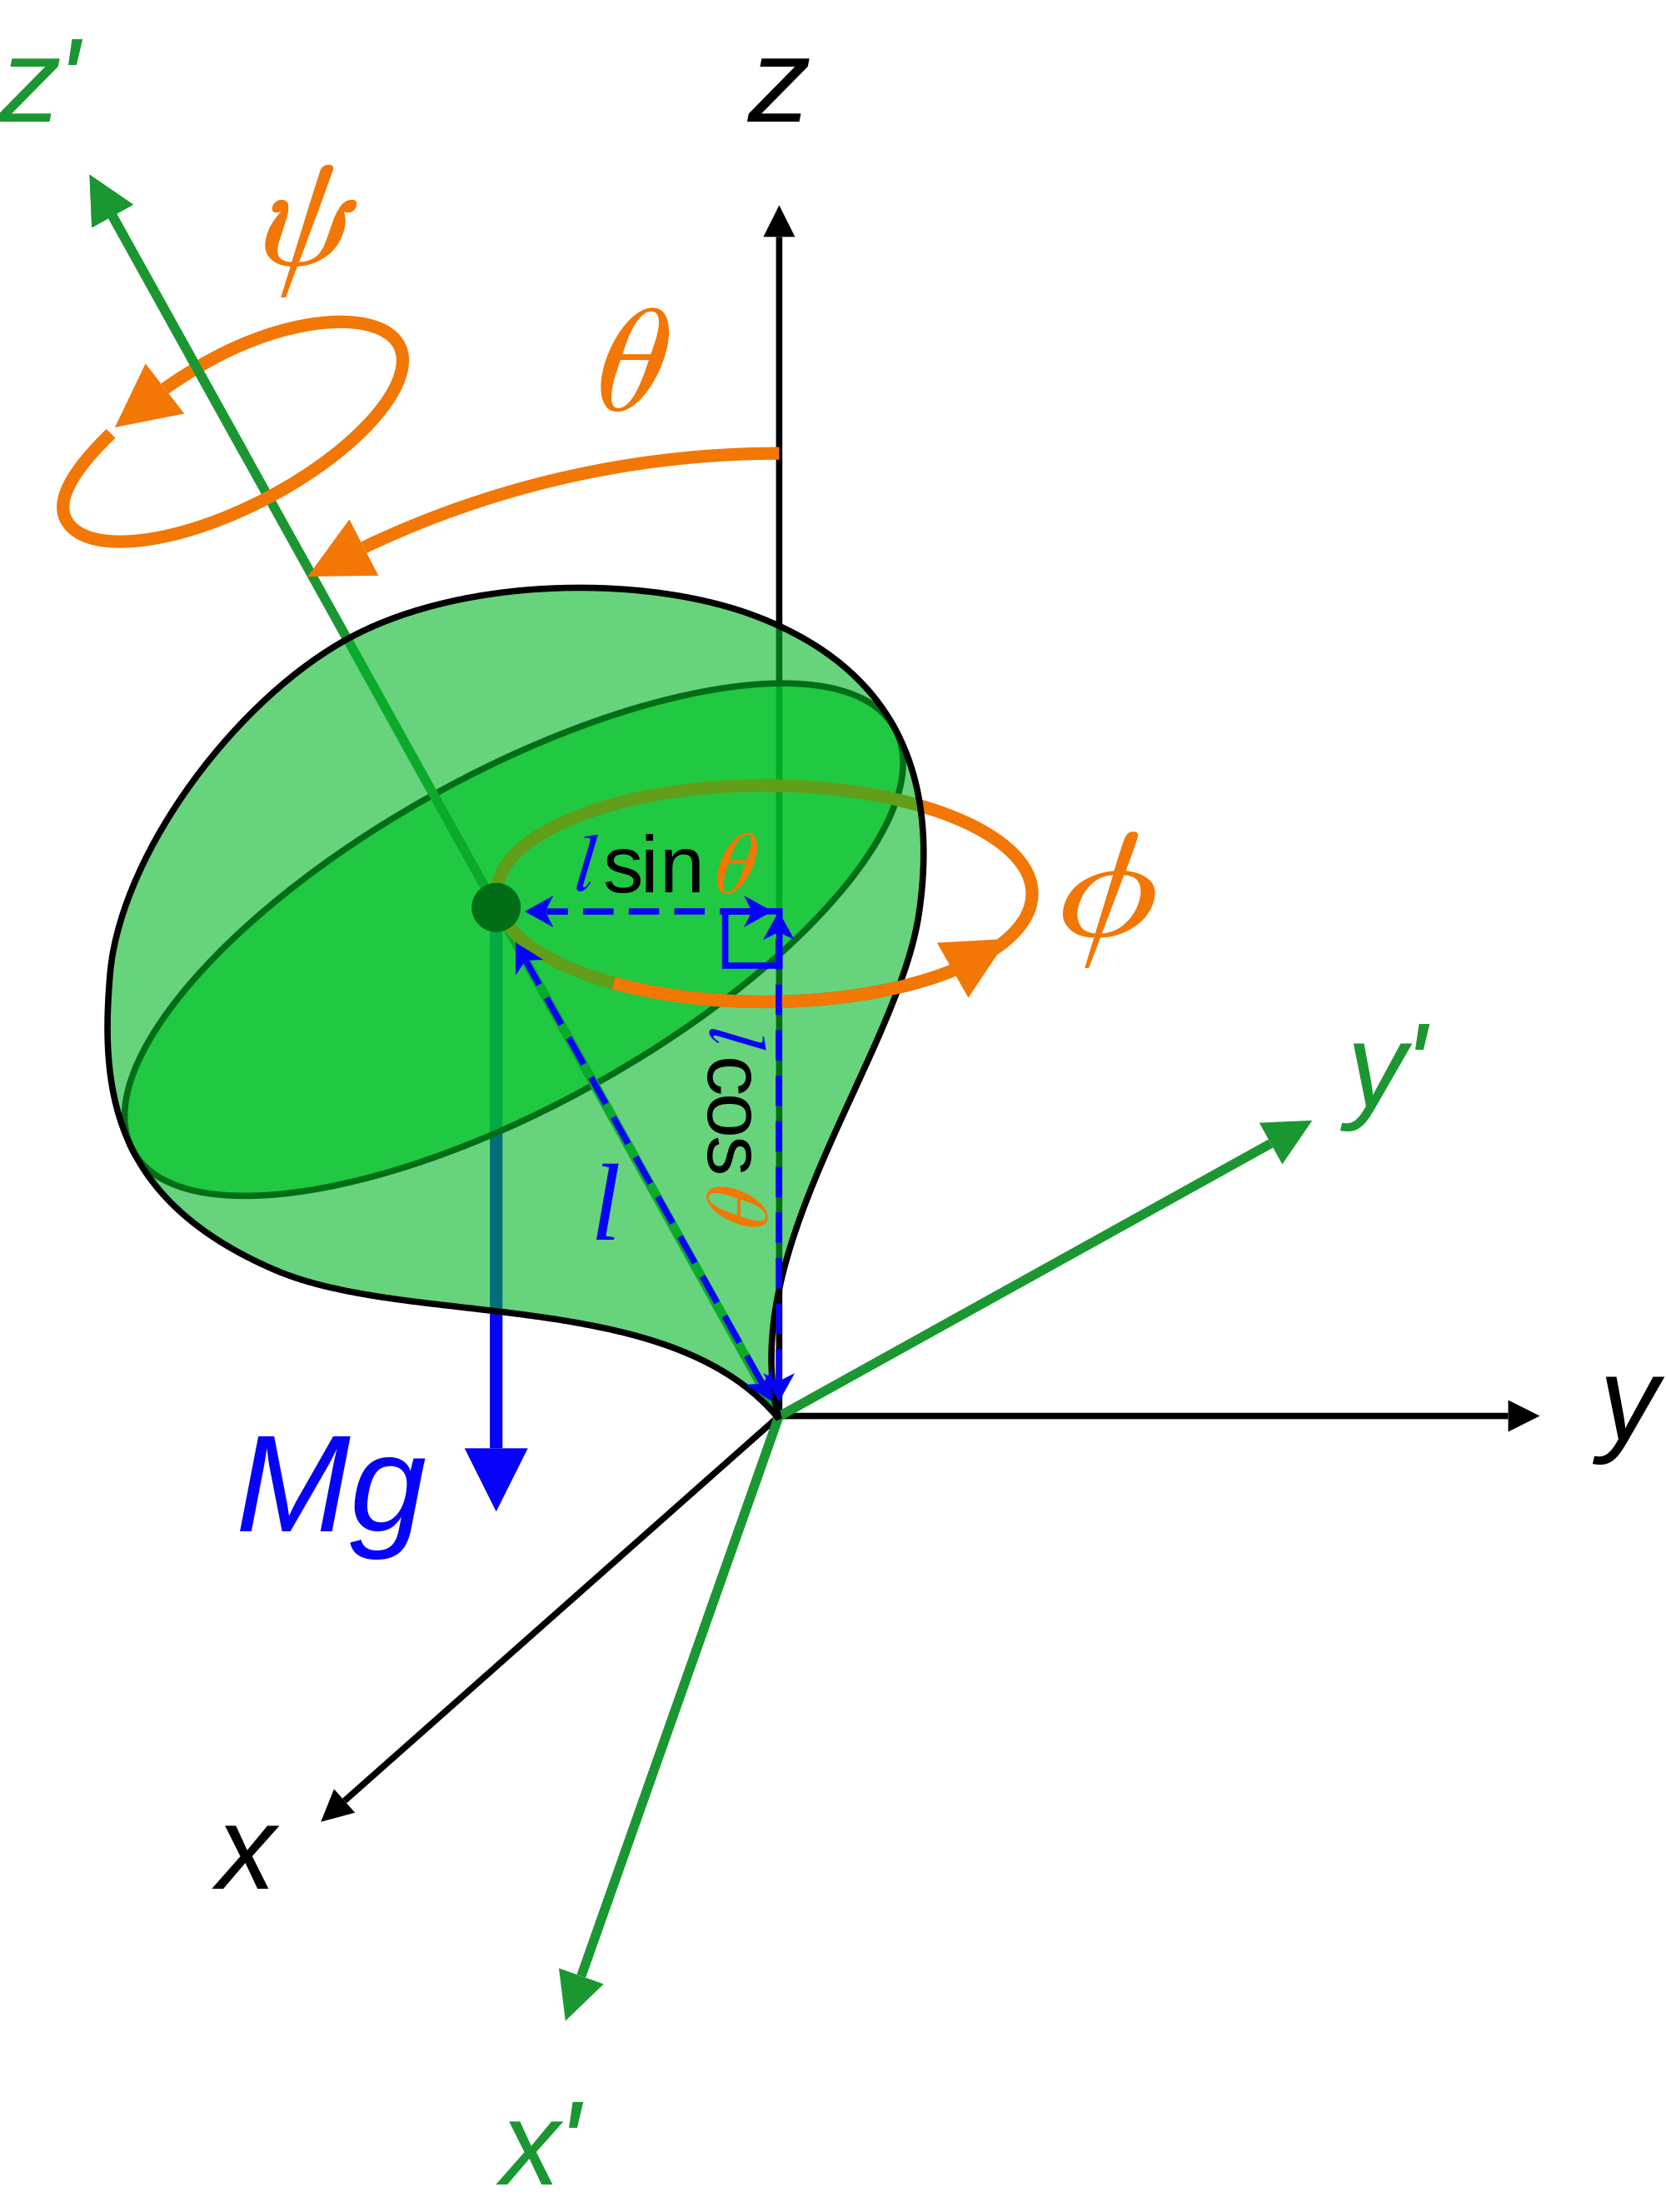
\includegraphics[width=\textwidth]{pics/eulertop}
    \caption{Trompo simétrico. Fuente: \cite{eulertop}.}
  \end{minipage}
  \end{figure}

  Inmediatamente tenemos
  \begin{align*}
    \dot{p_{\phi}} = & \parcial{H}{\phi} = 0 \\
    \dot{p_{\psi}} = & \parcial{H}{\psi} = 0,
  \end{align*}
  luego $p_{\phi}$ y $p_{\psi}$ son cantidades conservadas y por tanto su corchete de Poisson con $H$ se anula. Además, 
  \begin{equation*}
    \pois{p_{\phi}}{p_{\psi}} = 0.
  \end{equation*}
  Por tanto, $H$, $p_{\phi}$ y $p_{\psi}$ son funciones en involución en $(T^*\mathrm{SO}(3),H)$.

  Ahora, si estas funciones son constantes, como los ángulos (y sus relaciones trigonométricas) siempre están acotados también lo estará $p_{\theta}$ por la relación $E=H$ y la variedad $F^{-1}(a)$ estará acotada. Como $F^{-1}(a)$ es cerrada, es compacta y el trompo simétrico es «casi» un sistema integrable en el sentido de Liouville. Este «casi» viene porque, al igual que en el caso del péndulo habrá que exceptuar algún caso en el cual las funciones no son independientes.
\end{ejemplo}

\begin{ejemplo}
  \em
  Por citar un ejemplo no trivial, aunque no lo demostremos, el problema de hallar las geodésicas en un elipsoide puede verse como un sistema hamiltoniano integrable en el sentido de Liouville. La demostración se basa en la teoría de cuádricas confocales y coordenadas elípticas, demostrando unos teoremas de Jacobi y Chasles. Puede leerse en el apéndice 15 de \cite{arnold}.
\end{ejemplo}

Comenzaremos ahora a probar los resultados fundamentales de esta teoría. En primer lugar, vamos a obtener una caracterización general de los toros, que necesitaremos más adelante:

\begin{prop}
  Sea $M$ una variedad diferenciable de dimensión $n$ conexa y compacta tal que existen campos $X_1,\dots,X_n$ en $M$ linealmente independientes y tales que, para todo $i,j=1,\dots,n$, $i\neq j$, $[X_i,X_j]=0$. Entonces $M$ es difeomorfa al toro $n$-dimensional 
  \[
  \mathbb{T}^n=\mathbb{S}^1\times \dots \times \mathbb{S}^1.
  \]
  \label{Toros}
\end{prop}
\begin{proof}
  Para cada $i=1,\dots,n$, sea $g_i$ el flujo cuyo generador infinitesimal es $X_i$. Como para todo $i\neq j$, $[X_i,X_j]=0 $ entonces $g_i$ conmuta con $g_j$, es decir, $g_ig_j (x)=g_jg_i (x)$, para todo $x \in M$. 

  Así, podemos definir una acción de $\RR^n$ en $M$ que a cada $t=(t_1,\dots,t_n)\in \RR^n$ le asigna $g_t:M\rightarrow M,$ con $g_t=g_{1,t_1}\cdots g_{n,t_n}$.
Claramente, dados $t,s \in \RR^n$, $g_{t+s}=g_t g_s$. Ahora, fijo $x_0 \in M$, definimos 
\[
  \begin{array}{rcl}
g:\RR^n & \longrightarrow & M \\
t & \longmapsto & g_t (x_0).
\end{array}
\]

\nota{Esto hay que verlo bien (Problemas 1 y 2 de la 274 del Arnold).} Como los campos son linealmente independientes, $d_0 g$ es un isomorfismo lineal y, por el teorema de la función implícita, $g$ es un difeomorfismo local. Además, sea $x\in M$, tomamos una curva $\gamma$ que una $x$ y $x_0$ y una sucesión finita de entornos $V_1,\dots,V_n$ que recubran $\gamma$, en los que $g$ sea difeomorfismo y tales que $x_0 \in V_1$, $x \in V_n$. Para cada $i=1,\dots,n-1$, sea $x_i \in V_i \cap V_{i+1}$ y sea $x_n=x$. Para cada $i=0,\dots,n-1$, centramos $g$ en $x_i$ (de tal forma que $g(0)=x_i$) en el entorno $V_{i+1}$ y lo llamamos $g_i$. Definimos $t_i$ tal que $g_{i-1,t_i}(x_{i-1})=x_i$, entonces,
\[
  x=g_{n-1,t_n}(x_{n-1})=g_{n-1,t_n}g_{n-2,t_{n-1}}(x_{n-2})=\cdots=g_{n-1,t_{n}}\cdots g_{0,t_1} (x_0),
\]
luego, sea $t=t_1+\cdots+t_n$, $x=g_t (x_0)$. Por tanto, $g$ es sobreyectiva.
\begin{figure}[h]
  \centering
  \includegraphics[width=0.5\textwidth]{pics/entornos.eps}
  \caption{Idea de la demostración de que $g$ es sobreyectiva.}
  \label{fig:entornos}
\end{figure}

  Si $g$ fuese inyectiva, entonces sería un difeomorfismo entre $\RR^n$ y $M$, pero no puede serlo porque $M$ es compacta y $\RR^n$ no lo es.

  Por tanto, sea 
\[  
  H:=\{t \in \RR^n \mid g_t(x_0)=x_0\},
\]
entonces $H \neq {0}$. Ahora, sean $t, s \in H$, entonces 
\[
  g_{s+t}(x_0)=g_sg_t(x_0)=g_s(x_0)=x_0
\]
y 
\[
  g_{-t}(x_0)=g_{-t}g_t(x_0)=(x_0).
\] 
Es decir, $H$ es un subgrupo de $(\RR^n,+)$. Además, $H$ no depende de la elección de $x_0$, en efecto, si $x=g_r (x_0)$ y $t\in H$, entonces 
\[
  g_t (x) = g_{t+r}(x_0)=g_rg_t(x_0)=g_r(x_0)=x. 
 \] 

 Como $g$ es un difeomorfismo local, existe un entorno $V\subset \RR^n$ de 0 tal que $H\cap V= \{0\}$. Es más, sean $t\in H$, $s\in V\backslash \{0\}$ y $x\in M$, 
  \[
    g_{t+s}(x)=g_sg_t(x)=g_s(x)\neq x.
  \]
  Luego $H$ es un conjunto discreto.
  \begin{figure}[h]
    \centering
    \includegraphics[width=0.2\textwidth]{pics/discreto}
    \caption{Idea de que $H$ es discreto.}
    \label{fig:discreto}
  \end{figure}

  Antes de continuar, es necesario probar el siguiente lema:

  \begin{lema}
    Todo subgrupo discreto no trivial $H$ de $\RR^n$ es isomorfo a $\ZZ^k$ para algún $k\in\{1,\dots,n\}$. Es decir, existen $e_1,\dots,e_k \in H$ linealmente independientes tales que 
    \[
      H=\{n_1e_1+\cdots+n_ke_k \mid (n_1,\dots,n_k) \in \ZZ^k \}.
    \]
  \end{lema}
  \begin{proof} 
  Sea $e_0 \in H$, $e_0 \neq 0$. Como $H$ es discreto, $H \cap B(0,\norm{e_0})$ es finito. De estos puntos, consideramos aquellos que están en $L(e_0)$ \footnote{Aquí $L(x)$ denota la envoltura lineal de $x$.} y de estos escogemos el más cercano, que llamaremos $e_1$. 
  
  Si existieran algún $e \in H$ y algún $m \in \ZZ$ tal que $e \in (me_1,(m+1)e_1)$, entonces $e-me_1 \in H \cap L(e_0)$ estaría más cerca de 0 que $e_1$. Por tanto, 
  \[
    H\cap L(e_0) = e_1\ZZ.
  \]

  Si no hay puntos de $H$ fuera de $L(e_1)$ hemos terminado, $H$ es isomorfo a $\ZZ$. En caso contrario, sea $e \in H \backslash L(e_1)$, proyectamos ortogonalmente $e$ sobre $L(e_1)$. Esta proyección cae exactamente sobre un intervalo $\Delta=[me_1,(m+1)e_1)$ para cierto $m \in \ZZ$. Sea $C$ el cilindro de eje $\Delta$ y de radio igual a la distancia entre $\Delta$ y $e$. $C\cap H$ es finito. De estos puntos, sea $e_2$ el más cercano a $\Delta$ que no esté en $\Delta$. Entonces, para cualquier otro $f \in H$, la distancia entre $f$ y $L(e_1)$ es mayor que la distancia entre $e_2$ y $L(e_1)$. 
    
    En efecto, en tal caso, sea $l \in \ZZ$ tal que la proyección ortogonal de $f$ cae sobre $[le_1,(l+1)e_1)$, entonces $f'=f-le_1+me_1 \in C$ y la distancia entre $f'$ y $L(e_1)$ es menor que la distancia entre $e_2$ y $L(e_1)$, lo que nos lleva a una contradicción.

  \begin{figure}[h]
    \centering
    \includegraphics{pics/grupo}
    \caption{Idea de la demostración del lema.}
    \label{fig:grupo}
  \end{figure}

      Ahora, $\{n_1e_1+n_2e_2 \mid (n_1,n_2) \in \ZZ^2 \}$ forma una red discreta en $L(e_1,e_2)$. Además, si existiera un $e\in H$ que no perteneciese a la red, sean $m_1=[\esc{e}{e_1}]$, $m_2=[\esc{e}{e_2}]$. Entonces, $e-m_1e_1-m_2e_2$ estaría más cerca de $L(e_1)$ que $e_2$. Por tanto, esta red es exactamente $L(e_1,e_2) \cap H$.

      Procedemos ahora por inducción, supongamos que existen $e_1,\dots,e_k$ linealmente independientes tales que $\{n_1e_1+\cdots+n_ke_k \mid (n_1,\dots,n_k) \in \ZZ^k \} = L(e_1,\dots,e_k) \cap H$ y que existe $e\in H$ tal que $e \not\in L(e_1,\dots,e_k)$. Análogamente, la proyección ortogonal de $e$ sobre $L(e_1,\dots,e_k)$ cae sobre un hipercubo $\Delta=[m_1e_1,(m_1+1)e_1) \times \cdots \times [m_ke_k,(m_k+1)e_k)$. Sea $C$ el conjunto de los puntos cuyas proyecciones ortogonales caen en $\Delta$ y más cercanos a $\Delta$ que $e$, entonces $C \cap H$ es finito. Sea $e_{k+1}$ el más cercano a $\Delta$ de estos puntos, que no esté en $\Delta$. Para cualquier otro $f \in H$, la distancia entre $f$ y $L(e_1,\dots,e_k)$ es mayor que entre $e_2$ y $L(e_1,\dots,e_k)$, por un razonamiento completamente análogo al caso bidimensional. 

	Por tanto, $\{n_1e_1+\dots+n_{k+1}e_{k+1} \mid \in \ZZ^{k+1}\}$ forma una red discreta en $L(e_1,\dots,e_{k+1})$ y, de forma análoga al caso anterior, esta red agota los puntos de $H\cap L(e_1,\dots,e_{k+1})$.

	Finalmente, sea $k$ el mínimo número natural tal que no existe $e \in H \backslash L(e_1,\dots,e_k)$. Entonces $H$ es isomorfo a $\ZZ^k$.
\end{proof}

Terminamos ahora la demostración de la proposición.
 
  Sea $k$ el número de generadores de $H$ y sea la proyección natural
  \[
    \begin{array}{rcl}
      p: \RR^n = \RR^k \times \RR^{n-k} & \longrightarrow & \TT^k \times \RR^{n-k} \\
      (x,y) & \longmapsto & (x\mod  2\pi, y),
    \end{array}
  \]
  los puntos $u_1,\dots,u_k \in \RR^n$ de la forma 
  \[
    u_i = (x_1=0,\dots,x_i=2\pi,\dots,x_k=0,y=0)
  \]
  van a 0 por esta aplicación.

  Sean $e_1,\dots,e_k$ los generadores de $H$ y sea $A:\RR^n \rightarrow \RR^n$ un isomorfismo tal que cada $u_i$ va a parar a $e_i$. Entonces, la aplicación $\tilde{A}$ dada por el siguiente diagrama es un difeomorfismo.
  
\begin{center}
\begin{tikzpicture}[scale=2]
\node (A) at (0,1) {$\RR^n$};
\node (B) at (1,1) {$\RR^n$};
\node (C) at (0,0) {$\TT^k \times \RR^{n-k}$};
\node (D) at (1,0) {$M$};
\path[->,font=\scriptsize,>=angle 90]
(A) edge node[above]{$A$} (B)
(A) edge node[left]{$p$} (C)
(B) edge node[right]{$g$} (D)
(C) edge node[above]{$\tilde{A}$} (D);
\end{tikzpicture}
\end{center}
\nota{Probar que es un difeomorfismo}

Como por hipótesis $M$ es compacta, necesariamente $k=n$ y $M$ es difeomorfa a $\TT^n$.
\end{proof}

Podemos probar ahora el resultado fundamental de esta teoría:
\begin{thm}[Arnold]
Sea $(M,H)$ un sistema integrable en el sentido de Liouville. Entonces:
\begin{enumerate}
  \item $M_a$ es una variedad diferenciable invariante bajo el flujo de hamiltoniano $H=F_1$ y $\omega|M_a=0$.
  \item Cada componente conexa $C_a$ de $M_a$ es difeomorfa al toro n-dimensional 
    \[
      \TT^n=\SF^1 \times \cdots \times \SF^1
    \]
    y, sean $\theta=(\theta_1,\dots,\theta_n)$ coordenadas angulares en $C_a$, entonces existen unas frecuencias constantes $\omega(a)=(\omega_1(a),\dots,\omega_n(a))$ tales que
    \[
    \dot{\theta}(t)=\omega.
    \]
    
\end{enumerate}

\end{thm}

\begin{proof}
  En primer lugar, como las $n$ funciones $F_i$ son independientes en cada punto de $M_a$, por el teorema de la función implícita $M_a$ es una subvariedad regular de $M$ de dimensión $2n-n=n$. 
  Como $M$ es una variedad simpléctica, para cada $i=1,\dots,n$, podemos definir el campo $X_i=X^{F_i}=I \dd F_i$. Al ser las $\dd F_i$ linealmente independientes e $I$ un isomorfismo lineal, los campos $X_i$ son linealmente independientes. Además, por el teorema de Noether, como para cada $i,j= 1,\dots,n$ $\pois{F_i}{F_j}=0$ (luego es constante), entonces $\lie{X_i}{X_j}=0$. Por esto mismo, la derivada de la función $F_i$ en la dirección de $X_j$ es 0, luego los campos $X_j$ son tangentes a $M_a$.

  De aquí sacamos varias conclusiones:
  \begin{enumerate}
    \item $M_a$ es invariante con respecto a cada uno de los $n$ flujos hamiltonianos generados por cada función $F_i$ (luego, en particular lo será respecto del generado por $F_1$).
    \item Como, para cada $x \in M_a$, los campos $X_1|_x,\dots, X_n|_x$ forman una base de $T_x M_a$, sean $X_x, Y_x \in T_x M_a$, entonces $X_x = \sum_{i=1}^n b_i X_i|_x$, $Y_x=\sum_{i=1}^n c_i X_i|_x$. Ahora,
      \[
	\omega(X_x,Y_x)= \sum_{i,j=1}^n b_i c_j \omega(X_i|_x,X_j|_x) = \sum_{i,j=1}^n b_i c_j \{F_j,F_i\} = 0.
      \]
      Por tanto, $\omega$ se anula en $T_x M_a$. 
    \item $M_a$ es una variedad diferenciable de dimensión $n$ con $n$ campos conmutativos dos a dos y linealmente independientes en todo punto de $M_a$. 
  \end{enumerate}

Por esto último, por la proposición anterior y porque $M_a$ es compacta tenemos que cada componente conexa $C_a$ de $M_a$ es difeomorfa a $\TT^n$. De la demostración de la proposición anterior obtenemos un diagrama de la forma:

\begin{center}
\begin{tikzpicture}
\node (A) at (-2.5,2) {$\RR^n$};
\node (B) at (-1,2) {$\RR^n$};
\node (C) at (-1,0) {$C_a=\TT^n$};
\node (D) at (1,2) {$\theta$};
\node (E) at (3,2) {$t$};
\node (F) at (3,0) {$\theta \mod 2\pi$};
\path[->,font=\scriptsize, >=angle 90]
(A) edge node[above]{$A$} (B)
(A) edge node[left]{$p$} (C)
(B) edge node[right]{$g$} (C);
\path[|->,font=\scriptsize, >=angle 90]
(D) edge node[auto] {$$} (F)
(D) edge node[auto] {$$} (E)
(E) edge node[auto] {$$} (F);
\end{tikzpicture}
\end{center}


En este caso, el flujo hamiltoniano asociado a $F_1$ es $g_1$, luego 
\[
\theta(t) = g_{1,t} (\theta(0)).
\]
Ahora, fijo $\theta(0)$, $g_{1,t}=g(t,0,\dots,0)$, por tanto
\[
\left(
\begin{array}{c}
\theta_1 (t)\\
\vdots \\
\theta_n (t)
\end{array}
\right)
=
A
\left(
\begin{array}{c}
t\\
0 \\
\vdots \\
0
\end{array}
\right).
\]
De modo que, si $a_{ij}$ es la entrada de índices $(i,j)$ de la matriz $A$, entonces, para cada $i=1,\dots,n$,
\[
\theta_i (t) = a_{i1} t.
\] 
Por tanto, sea $\omega_i=a_{i1}$,
\[
\dot{\theta_i}(t)=\omega_i.
\]
\end{proof}

\begin{obs}
  \em
  Estas subvariedades $C_a$ de $M$ se suelen llamar \textit{toros invariantes} del sistema $(M,H)$. 
  Esta dinámica en el toro recibe el nombre de \emph{movimiento condicionalmente periódico}.
\end{obs}

\begin{obs}
  \em
  Consideremos un 2-toro invariante con la dinámica del teorema (por ejemplo, el asociado a los niveles de energía de un oscilador armónico bidimensional). Sea $(\theta_1,\theta_2)$ un punto en el toro y su trayectoria bajo el flujo hamiltoniano $\gamma(t)=\varphi_t(\theta_1,\theta_2)=(\theta_1+\omega_1t,\theta_2+\omega_2t)$. Si $\omega_1/\omega_2=m/n$ es racional, entonces 
  \begin{equation*}
    \gamma\left(\frac{2n\pi}{\omega_2}\right) = (\theta_1+2m\pi,\theta_2+2n\pi)=(\theta_1,\theta_2).
  \end{equation*}
  Es decir, a cierto tiempo la trayectoria «se cierra». Estas órbitas se dicen \emph{periódicas}. 
 
  Sin embargo, si $\omega_2/\omega_1$ es irracional, dado un ángulo $\alpha$ y sea $T$ tal que $\alpha=\theta_1+\omega T$, entonces, sea $T_n=T+2n\pi/\omega_1$, $\alpha=\theta_1+\omega_1(T_n)$ para cada $n\in \NN$. Sea ahora la aplicación
  \begin{equation*}
    \begin{array}{rcl}
    g:\SF^1 & \longrightarrow &\SF^1 \\
  \phi & \longmapsto & \phi + 2\pi\frac{\omega_2}{\omega_1},
  \end{array}
\end{equation*}
es una rotación de ángulo un múltiplo irracional de $2\pi$ en la circunferencia del toro de ángulo $\alpha$. Entonces, como ya vimos por el teorema de recurrencia de Poincaré, $\{g^n(\phi)|n\in \NN\}$ es denso en $\SF^1$. Como esto es válido para todo $\alpha$ y se cumple 
\begin{equation*}
  \gamma(T_n)=(\alpha,g^n(\theta_2)+\omega_2 T),
\end{equation*}
tenemos que $\{\gamma(t)|t \in \RR \}$ es denso en el toro. Este tipo de órbitas se llaman \emph{cuasiperiódicas}. Una forma sencilla de visualizar esto es mediante las \emph{figuras de Lissajous} 
\begin{equation*}
  L_{\omega}=\{(\cos t, \cos \omega t) | t \in \RR\},
\end{equation*}
ver figura \ref{fig:lissajous}.
\begin{figure}[h]
  \centering
  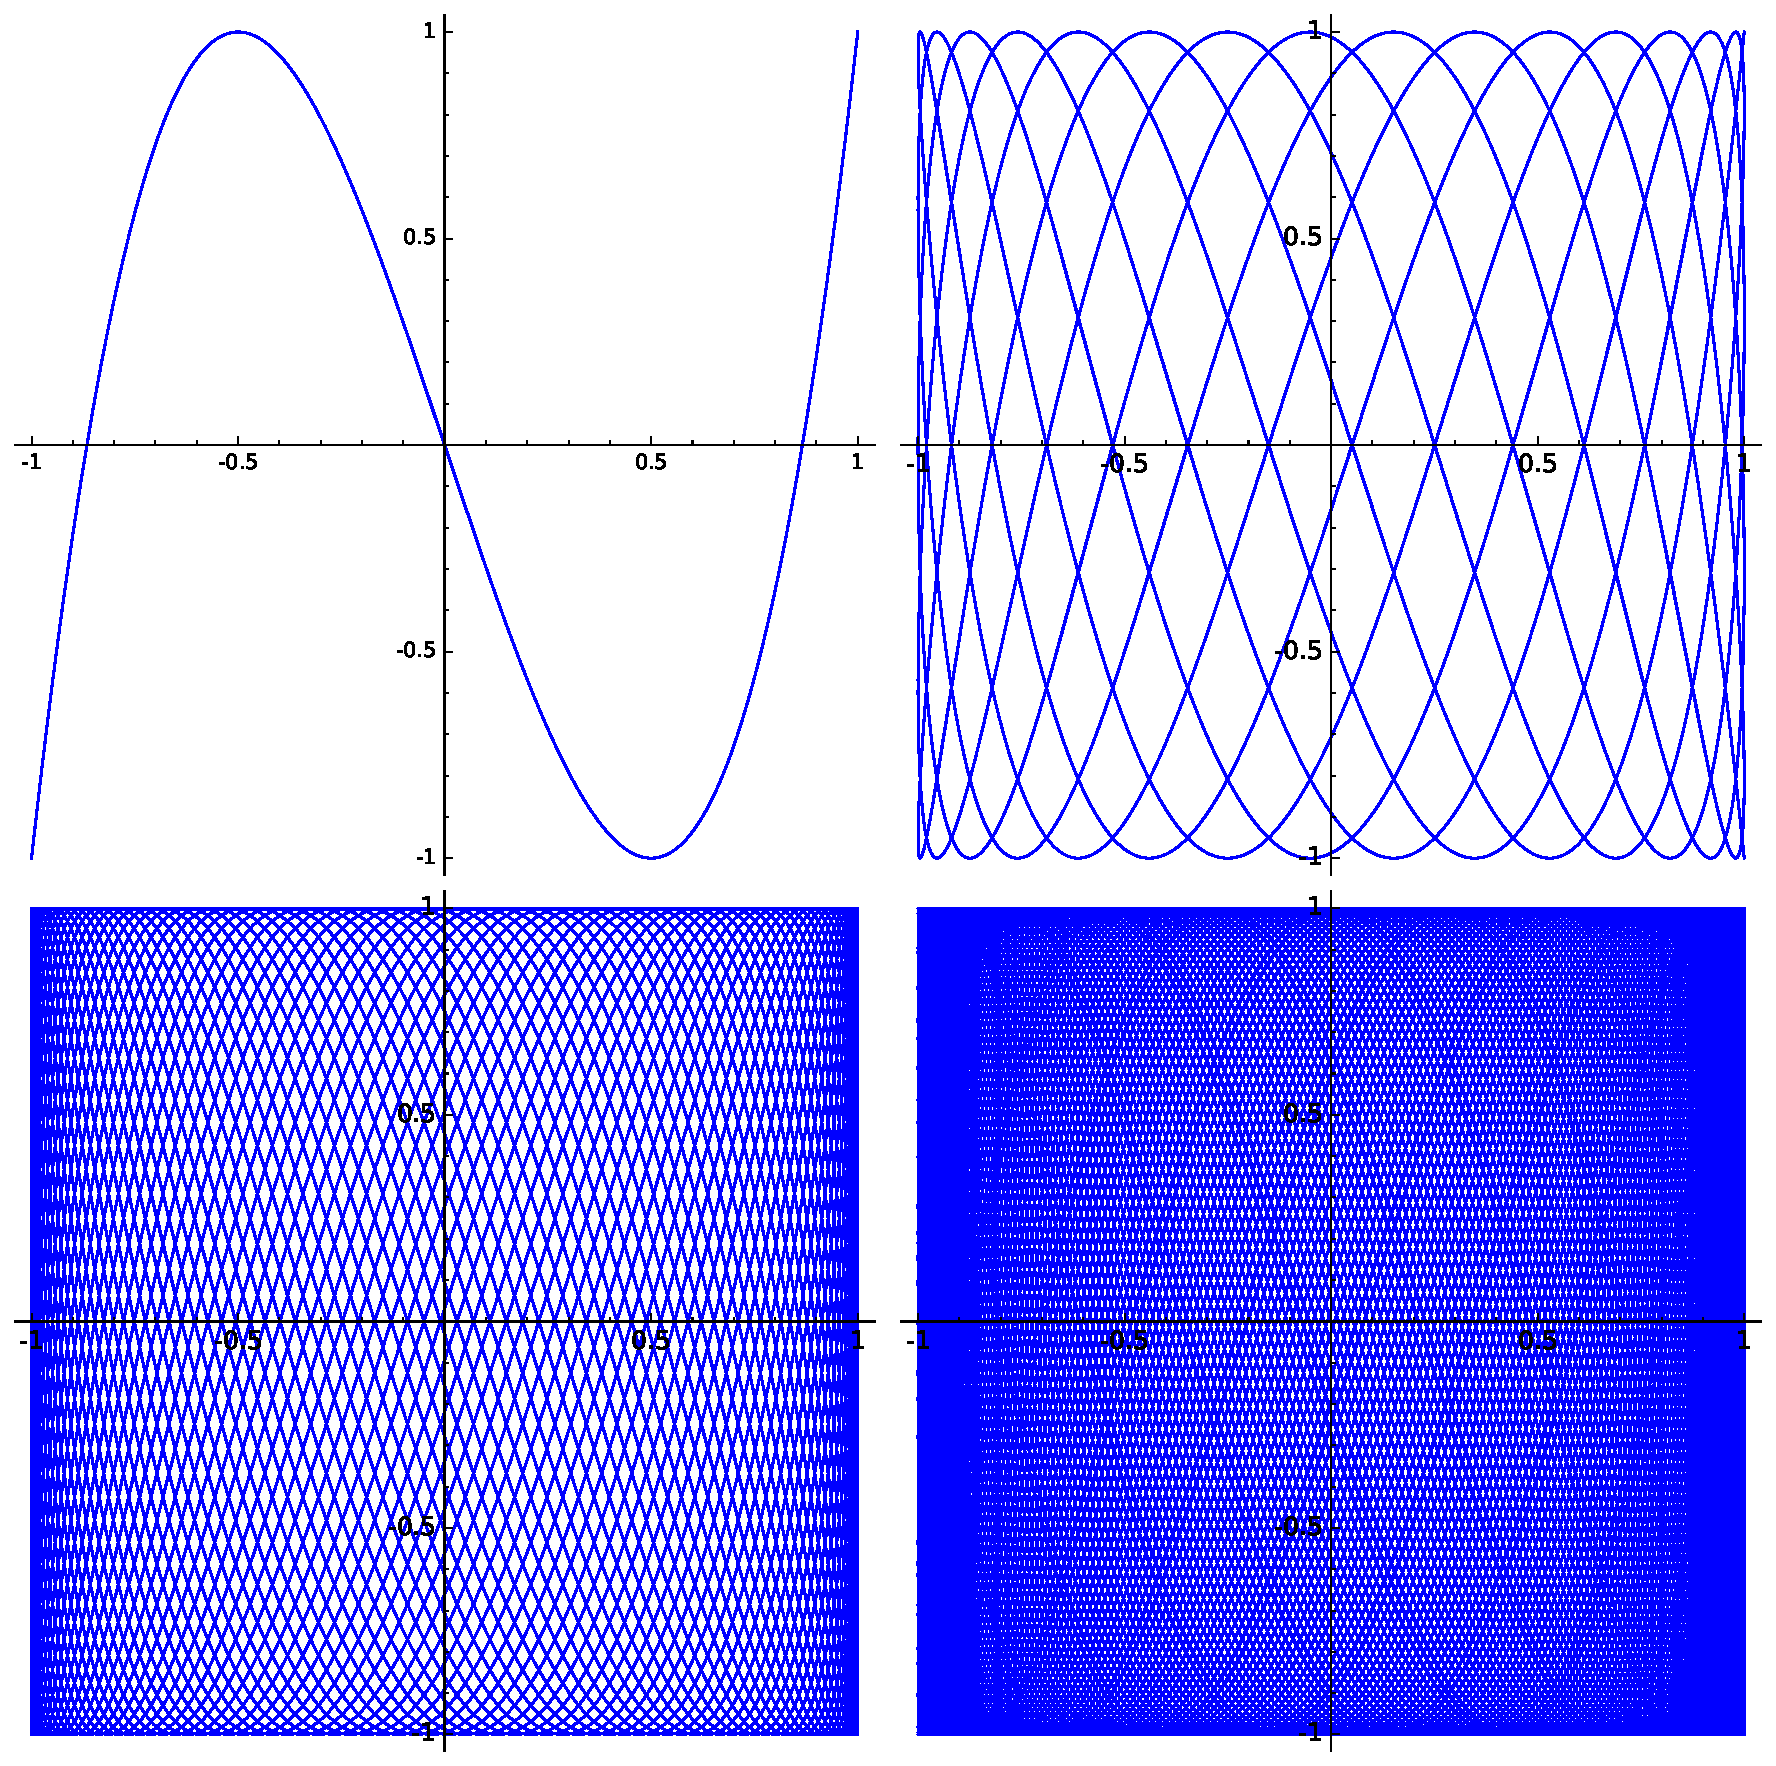
\includegraphics[width=0.6\textwidth]{pics/lissajous}
  \caption{Figuras de Lissajous para $\omega=3;3.1;3.14;3.1416$, $t \in (0,128\pi)$ con pasos de $0.01$.}
  \label{fig:lissajous}
\end{figure}
\end{obs}

Si $(M,H)$ es integrable en el sentido de Liouville, entonces para todo $x \in M$, $M_{F(x)}$ es compacta, luego la componente conexa a la que pertenezca $x$, $C_{F(x)}$, es un toro invariante, en el que podemos dar coordenadas angulares con una dinámica como la del teorema. A la vista de esto, tenemos el siguiente corolario:

\begin{corol}
  Sea (M,H) un sistema integrable en el sentido de Liouville, $a \in \RR^n$ y $C_a$ un toro invariante. Existe un $U \subset M$ entorno de $C_a$ difeomorfo a $\RR^n \times \TT^n$. 
\end{corol}

\begin{proof}
  \nota{Cuidado con ésta que la he escrito yo.}
  Por hipótesis, las $F_i$ son independientes para todo $x \in M$, luego $F_*$ tiene rango máximo. Por tanto, sea $x$ tal que $F(x)=a$, existe $D\simeq \RR^{2n}$ entorno simplemente conexo de $x$, existe $V\subset D$ y existe $B\subset \RR^n$ abierto tal que $F|V:V \rightarrow B$ es un difeomorfismo. Ahora, sea
  \[
    \begin{array}{rcl}
      \Phi:M & \longrightarrow & \RR^n \times \TT^n \\
           x & \longmapsto & (F(x), \theta),
    \end{array}
  \]
  con $\theta$ coordenadas angulares en $C_{F(x)}$ el toro invariante al que pertenece $x$. Entonces claramente $\Phi$ da un difeomorfismo entre $U=\bigcup_{x\in V}C_{F(x)}$ (que es un entorno de $C_a$) y $\bigcup_{b \in B} C_b$. Como $B$ es un abierto de $\RR^n$ y $C_b$ es un toro invariante, $U$ es difeomorfo a $\RR^n \times \TT^n$.
\end{proof}
\begin{obs}
  \em
  Aquí estamos suponiendo que $x$ no está en el borde de $M$, en tal caso procederíamos análogamente para obtener un entorno difeomorfo a $\HH^n \times \TT^n$.
\end{obs}

Finalmente, vamos a demostrar el teorema clave que nos permite construir la carta en la cual las ecuaciones de Hamilton pueden ser integradas por cuadraturas.
\begin{thm}[de las variables de acción-ángulo]
  Sea $(M,H)$ un sistema integrable en el sentido de Liouville, $D \in \RR^n$ un disco, $a \in \RR^n$, $C_a$ un toro invariante y $U$ un entorno de $C_a$ difeomorfo a $\RR^n \times \TT^n$. Entonces existe un sistema de coordenadas simplécticas $(\phi,J)=(\phi_1,\dots,\phi_n,J_1,\dots,J_n)$ en $U$ tales que las $\phi_i$ son coordenadas angulares en cada toro invariante y las $J_i$ (comúnmente llamadas \emph{variables de acción}) son constantes en estos toros.
\end{thm}
\begin{proof}
  Sea $\pi:U\simeq \RR^n \times \TT^n \rightarrow \RR^n$ la proyección canónica, entonces $\pi^{-1}(x)$ es un toro invariante para cada $x \in D=\pi(U)$. En cada uno de estos toros, sean $X_i=X^{F_i}$ y $(F,\theta)$ las coordenadas obtenidas en el lema anterior,
\[
  \deriv{\theta_i} = \sum_{k=1}^n a_{ik}X_k,
\]
donde las $a_{ik}$ son funciones constantes en cada toro.

Como $\omega$ se anula en el toro, no tiene términos en $\dd \theta_i \wedge \dd \theta_j$. Los términos en $\dd \theta_i \wedge \dd F_j$ serán
\[
  \omega\left(\deriv{\theta_i},\deriv{F_j}\right)=\sum_{k=1}^n a_{ik}\cdot \omega\left(X_k,\deriv{F_j}\right)=\sum_{k=1}^n a_{ik} \cdot \dd F_k \left(\deriv{F_j}\right) = \sum_{k=1}^n a_{ik} \delta_{ij}= a_{ij}. 
\]
Por tanto, $\omega$ es de la forma
\[
  \omega = \sum_{i,j=1}^n a_{ij} \dd \theta_i \wedge \dd F_j + \sum_{i,j=1}^n b_{ij} \dd F_i \wedge \dd F_j,
\]
con $b_{ij}$ unas ciertas funciones. Además, como $\omega$ es cerrada, el término correspondiente a $\dd \theta_k \wedge \dd F_i \wedge \dd F_j$ debe anularse. Este término es exactamente
\[
  \parcial{a_{ki}}{F_j}-\parcial{a_{kj}}{F_i}+\parcial{b_{ij}}{\theta_k}.
\]
El término $\parcial{a_{ki}}{F_j}-\parcial{a_{kj}}{F_i}$ no depende de las variables angulares, luego las $\parcial{b_{ij}}{\theta_k}$ son constantes al variar los ángulos $\theta_k$. Como las variables $\theta_k$ son angulares, las $b_{ij}$ deben ser periódicas, luego
\[
  \parcial{b_{ij}}{\theta_k}=0
\]
y las $b_{ij}$ son constantes en cada toro invariante.

Si ahora definimos $A_i=\sum_{j=1}^n a_{ij}\dd F_j$, $B=\sum_{i,j=1}^n b_{ij}\dd F_i \wedge \dd F_j$,
\[
  \omega=\sum_{i=1}^n \dd \theta_i \wedge A_i + B.
\]
Como las $a_{ij}$ y las $b_{ij}$ son constantes en cada toro invariante podemos ver las $A_i$ y $B$ como formas en $\RR^n$, es decir, existen 1-formas $\alpha_i$ y una 2-forma $\beta$ en $\RR^n$ tales que
\[
  A_i= \pi^* \alpha_i \hspace{1cm} B=\pi^* \beta.
\]
De aquí tenemos
\[
  0=\dd \omega= \sum_{i=1}^n \dd \theta_i \wedge \pi^* \dd \alpha_i + \pi^* \dd \beta,
\]
de donde concluimos que $\dd \alpha_i = 0$ y $\dd \beta =0$. En $\RR^n$ todas las formas cerradas son exactas. Por tanto, existen $I_i$ y $\gamma$ en $\RR^n$ tales que $\alpha_i = \dd I_i$, $\beta= \dd \gamma$.

Finalmente, sean $J_i=(I_i \circ \pi)=\pi^* I_i$, tenemos que $\dd J_i = A_i$, luego
\[
  \omega = \sum_{i=1}^n \dd \theta_i \wedge \dd J_i + B.
\]
En el sistema de coordenadas $(\theta,F)$, la matriz asociada a $\omega$ es de la forma
\[
\left(
\begin{array}{c|c}
  0 & \parcial{J_i}{F_j} \\
  \hline 
  -\parcial{J_i}{F_j} & b_{ij}
\end{array}\right).
\]
Como $\omega$ es regular, el determinante de esta matriz es distinto de cero, luego $\det\left(\parcial{J_i}{F_j}\right)\neq 0$. Por tanto, $(\theta,J)$ es un sistema de coordenadas.

Ahora, si escribimos $\gamma= \sum_{i=1}^n g_i \dd I_i$, para algunas funciones $g_i:\RR^n \rightarrow \RR$, entonces podemos tomar unas nuevas coordenadas 
\[
  \phi_i= \theta_i + (g_i \circ \pi).
\]
En estas nuevas coordenadas
\[
\begin{split}
  \sum_{i=1}^n \dd \phi_i \wedge \dd J_i & = \sum_{i=1}^n \dd \theta_i \wedge \dd J_i + \sum_{i=1}^n \dd(g_i \circ \pi) \wedge J_i \\
   & =\sum_{i=1}^n \dd \theta_i \wedge \dd J_i + \sum_{i=1}^n \dd(g_i \circ \pi) \wedge \dd (I_i \circ \pi) \\
   & =\sum_{i=1}^n \dd \theta_i \wedge \dd J_i + \pi^* \dd \gamma = \sum_{i=1}^n \dd \theta_i \wedge A_i + B = \omega.
\end{split}
\]

Por tanto, hemos encontrado unas coordenadas simplécticas $(J,\phi)$, con las $J_i$ constantes en cada toro invariante y con las $\phi_i$ coordenadas angulares en estos toros.
\end{proof}

\begin{obs}
  \em
  Volviendo al caso del oscilador armónico $n$-dimensional, notamos que $\omega=\dd \alpha$, con $\alpha=\sum_{i=1}^n J_i \dd \phi_i$, entonces $J_i=\frac{1}{2\pi}\int_{\gamma_i}\alpha$.
\end{obs}

\begin{corol}
  Todo sistema integrable en el sentido de Liouville es integrable por cuadraturas.
\end{corol}

\begin{proof}
  Dado un punto $x \in M$, basta tomar unas variables de acción-ángulo (las $(J,\phi)$ del teorema). Entonces, como ya hemos visto, las soluciones de las ecuaciones de Hamilton en estas coordenadas quedan escritas en la forma
  \begin{align*}
    J_i(t) & = J_i (0) \\
    \phi_i(t) & = \phi_i(0) + \omega_i(F(0))t,
  \end{align*}
  para $i=1,\dots,n$, donde las frecuencias $\omega_i$ se obtuvieron en términos de funciones conocidas. Así, el sistema queda integrado por cuadraturas.
\end{proof}



%\section{Un poco más de movimiento condicionalmente periódico}\label{sec:promedios}
Como colofón, una vez tenemos a nuestra disposición la teoría de Arnold-Liouville, sabemos que el flujo en los toros invariantes de los sistemas integrables en el sentido de Liouville será condicionalmente periódico. En esta sección definiremos bien qué significa esto y obtendremos un teorema muy importante sobre este tipo de sistemas.

\begin{defn}[Movimiento condicionalmente periódico en $\TT^n$]
  \em
  Sean $\TT^n$ el toro n-dimensional y $\phi=(\phi_1,\dots,\phi_n)$ coordenadas angulares. Se entiende por un \emph{movimiento condicionalmente periódico} en el toro el flujo uniparamétrico dado por 
  \begin{equation*}
    \phi(t)=\phi(0)+\omega t
  \end{equation*}
  con $\omega=(\omega_1,\dots,\omega_n)$ \emph{frecuencias} constantes en el toro. Las frecuencias $\omega$ se dicen \emph{independientes} si, sea $k \in \ZZ^n$, entonces $\esc{k}{\omega}=0$ si y sólo si $k=0$.
\end{defn}
\begin{defn}[Promedios espacial y temporal]
  \em
  Sea $f:\TT^n \rightarrow \RR$ una función integrable Riemann,
  \begin{enumerate}
    \item El \emph{promedio espacial} de $f$ en $\TT^n$ es el número
      \begin{equation*}
	\bar{f}=\frac{1}{(2\pi)^n}\int_0^{2\pi} \cdots \int_0^{2\pi} f(\phi) d\phi_1,\dots,d\phi_n.
      \end{equation*}
    \item El \emph{promedio temporal} de $f$ en $\TT^n$ es la función
      \begin{equation*}
	f^*(\phi_0)=\lim_{T\rightarrow \infty} \int_0^{T}f(\phi_0+\omega t) dt,
      \end{equation*}
      definida en los puntos $\phi_0$ en los que exista el límite.
  \end{enumerate}
\end{defn}

\begin{thm}[Teorema de los promedios]
  Si $f:\TT^n \rightarrow \RR$ es una función integrable Riemann y las frecuencias $\omega$ son independientes, el promedio temporal está bien definido en todo el toro $\TT^n$ y coincide en todo punto con el promedio espacial.
\end{thm}
\begin{proof}
 Daremos la demostración en varios pasos:
 \begin{enumerate}
   \item Consideramos funciones de la forma $e^{i\esc{k}{\phi}}$, $k\in \ZZ^n$. Si $k=0$, entonces $\bar{f}=f=f^*=1$. Si $k\neq0$, $\bar{f}$ es una integral a periodos en funciones trigonométricas, luego es igual a 0. Por otra parte
     \begin{equation*}
       \int_0^T e^{i\esc{k}{\phi_0 + \omega t}} dt= e^{i\esc{k}{\phi_0}}\int_0^T e^{i\esc{k}{\omega}t}dt=e^{i\esc{k}{\phi_0}}\frac{e^{i\esc{k}{\omega}T}-1}{i \esc{k}{\omega}}.
     \end{equation*}
     Por tanto, el promedio temporal será
     \begin{equation*}
       \lim_{T\rightarrow \infty}\frac{e^{i\esc{k}{\phi_0}}}{i \esc{k}{\omega}}\frac{e^{i\esc{k}{\omega}T}-1}{T}=0.
     \end{equation*}
   \item Como los promedios dependen linealmente de $f$, también coincidirán para los polinomios trigonométricos
     \begin{equation*}
       f=\sum_{|k|<N}f_ke^{i\esc{k}{\omega}}.
     \end{equation*}
   \item Dado $\varepsilon >0$, si $f$ es continua y real por el teorema de Weierstrass podemos aproximarla por un polinomio trigonométrico $P$ que cumpla $|f-P|<\frac{1}{2}\varepsilon$. Sean $P_1=P-\frac{1}{2}\varepsilon$, $P_2=P+\frac{1}{2}\varepsilon$ entonces
     \begin{equation*}
       \bar{P_2}-\bar{P_1}=\frac{1}{(2\pi)^n}\int_{\TT^n} (P_2 - P_1) d\phi = \frac{1}{(2\pi)^n}\varepsilon (2\pi)^n= \varepsilon.
     \end{equation*}
   \item Dado $\varepsilon >0$, si $f$ es real e integrable Riemann, entonces existen dos funciones continuas $f_1,f_2$ tales que $f_1<f<f_2$ y $\int_{\TT^n}\frac{1}{(2\pi)^n}(f_2-f_1)d\phi<\frac{1}{3}\varepsilon$. Tomando ahora $P_1,P_2$ polinomios trigonométricos tales que $P_1<f_1<f_2<P_2$ y $\int_{\TT^n}\frac{1}{(2\pi)^n}(P_i-f_i)d\phi < \frac{1}{3}\varepsilon$, para $i=1,2$, entonces
     \begin{equation*}
       \bar{P_2}-\bar{P_1}=\frac{1}{(2\pi)^n}\int_{\TT^n} (P_2 - P_1) d\phi = \frac{1}{(2\pi)^n}\varepsilon (2\pi)^n= \varepsilon.
     \end{equation*}
   \item Por último, sea $\varepsilon>0$, entonces existen dos polinomios trigonométricos $P_1,P_2$ tales que $P_1<f<P_2$ y $\bar{P_2}-\bar{P_1}<\varepsilon$. Ahora, como $f<P_2$,
     \begin{equation*}
       \frac{1}{T}\int_0^T f(\phi(t))dt < \frac{1}{T}\int_0^T P_2(\phi(t))dt,
     \end{equation*}
     luego
     \begin{equation*}
       \left| \frac{1}{T}\int_0^T f(\phi(t))dt- \bar{f} \right| <\left| \frac{1}{T}\int_0^T P_2(\phi(t))dt- \bar{f} \right| < \left| \frac{1}{T}\int_0^T P_2(\phi(t))dt- \bar{P_2}\right| + |\bar{P_2}-\bar{f}|.
     \end{equation*}
     Pero, como $P_1<f<P_2$, por la monotonía de la integral $\bar{P_1}<f<\bar{P_2}$, luego $|\bar{P_2}-\bar{f}|<|\bar{P_2}-\bar{P_1}|<\varepsilon$. Además, como $P_2$ es un polinomio trigonométrico existe un $T_0$ tal que, si $T>T_0$
     \begin{equation*}
       \left| \frac{1}{T}\int_0^T P_2(\phi(t))dt- \bar{P_2}\right| < \varepsilon .
     \end{equation*}
     Finalmente, obtenemos lo que queríamos probar
     \begin{equation*}
       \left| \frac{1}{T}\int_0^T f(\phi(t))dt- \bar{f} \right| <\left| \frac{1}{T}\int_0^T P_2(\phi(t))dt- \bar{P_2}\right| + |\bar{P_2}-\bar{f}|<\varepsilon + \varepsilon = 2\varepsilon,
     \end{equation*}
     luego $f^*(\phi_0)=\lim_{t\rightarrow \infty}\frac{1}{T}\int_0^T f(\phi(t)) dt = \bar{f}$.
 \end{enumerate}
\end{proof}
\begin{corol}
  Si las frecuencias son independientes, entonces, para todo $\phi_0 \in \TT^n$, \[\{\phi(t)=\phi_0+\omega t|t\in \RR\}\] es denso en el toro $\TT^n$.
\end{corol}
\begin{proof}
  En caso contrario, sea un abierto $D$ del toro que no tiene ningún punto de la trayectoria $\phi(t)$. Construimos la función 
  \begin{equation*}
    f(\phi)=\left\lbrace
    \begin{array}{ll}
      0 & \text{si } \phi \not\in D \\
      \frac{(2\pi)^n}{\int_D d\phi} & \text{si } \phi \in D.
    \end{array}
    \right.
  \end{equation*}
  Claramente, $\bar{f}=1$, pero $f^*(\phi_0)=0$, lo que contradice el teorema de los promedios.
\end{proof}
\begin{corol}
  Sea $D\subset \TT^n$ un conjunto medible Jordan. Sea $A_D=\{t\in \RR | \phi(t) \in D\}$ (que también es medible Jordan) y sea $\tau_D(T)=\int_0^T\chi_{A_D}(t)dt$. Entonces
  \begin{equation*}
    \lim_{T\rightarrow \infty}\frac{\tau_D(T)}{T}= \frac{\mathrm{Vol}(D)}{(2\pi)^n}.
  \end{equation*}
\end{corol}
\begin{proof}
  Aplicamos el teorema a $\chi_D$, entonces $\int_0^T \chi_D(\phi(t))dt=\int_0^T \chi_{A_D}(t)dt=\tau_D(t)$ y $\bar{\chi}_D=(2\pi)^{-n}\mathrm{Vol}(D)$. Finalmente, por el teorema de los promedios
  \begin{equation*}
    \bar{\chi}_D=\frac{\mathrm{Vol}(D)}{(2\pi)^n}=\lim_{T\rightarrow \infty}\frac{1}{T}\int_0^T \chi_D(\phi(t))dt=\lim_{T\rightarrow \infty}\frac{\tau_D(T)}{T}.
  \end{equation*}
\end{proof}


\addcontentsline{toc}{chapter}{Bibliografía}
\nocite{*}
\bibliographystyle{plain}
\bibliography{biblio}

%\newpage\null\thispagestyle{empty}\newpage

%\chapter*{Agradecimientos}

%Al profesor Otto R. Campoamor por la revisión del trabajo, ayudando a aclarar toda la Física que hay detrás. 
%A Jesús M. Ruiz, mi tutor, por su atención incansable, su revisión minuciosa de todo lo que he escrito y, sobre todo, por su tremendo cariño a las Matemáticas y a las cosas bien hechas.

%A mis padres, Isabel y Javier, sin los cuales nada de esto sería posible.
%A mi hermana, Almudena, por aguantarme estos 5 años (y los otros 18).
%A mi tía Tere y a mi abuela Florencia, por hacer mi estancia en Madrid más cómoda y llevadera, por el cocido todos los sábados, y por haberme ayudado siempre que lo he necesitado. 

\end{document}




